\documentclass[12pt,a4paper]{report}
\usepackage[top=2.5cm, bottom=2.5cm, left=2.5cm, right=2.5cm]{geometry}

% - taille de la fonte    : 10pt, 11pt, 12pt
% - recto ou recto-verso  : oneside, twoside
% - stade de développement: draft, final

\usepackage[T1]{fontenc}
\usepackage[french]{babel}
\usepackage{textcomp}

\usepackage[pdftex]{graphicx}
\usepackage{setspace}
\usepackage[hypertexnames=false]{hyperref}
\usepackage{float}
\usepackage[french]{varioref}
\usepackage{fancyhdr}
\usepackage{color}
\usepackage{colortbl}
\usepackage{amsmath}
\usepackage{ifpdf}
\usepackage{array}
\usepackage{multirow}
\usepackage{subcaption}

\IfFileExists{lmodern.sty}{\usepackage{lmodern}}{}

\setlength{\headheight}{14pt}

\pagestyle{fancy}
\fancyhead[L]{\nouppercase\leftmark}
\fancyhead[C]{}
\fancyhead[R]{\nouppercase\rightmark}

\fancyfoot[L]{}
\fancyfoot[C]{}
\fancyfoot[R]{\textbf{\thepage}}

\begin{document}
%%%%%%%%%%%%% pages de garde en Français
\include{garde_fin}
\include{garde_sign_fin}

\newpage
\pagenumbering{roman}
\chapter*{Dédicaces}
\addcontentsline{toc}{chapter}{Dédicaces}

\noindent A mes parents,
\\
A ma famille,
\\
A mes amis 
\include{Remerciements}
\tableofcontents
\listoffigures
\listoftables
\newpage
\pagenumbering{arabic}

\chapter*{Introduction Générale}
\markboth{Introduction Générale}{} %pour afficher l'entete
\addcontentsline{toc}{chapter}{Introduction Générale}

Le harcèlement scolaire touche des centaines de milliers d'élèves chaque année.
Avec la généralisation d'Internet et des réseaux sociaux, il prend désormais une dimension numérique : le cyberharcèlement.
Les victimes reçoivent des insultes, des menaces et des humiliations en ligne, souvent de manière anonyme,
sans qu'aucun mécanisme ne soit disponible pour les détecter ou les accompagner en dehors des heures ouvrées.

\bigskip

Face à ce constat, la société Smart-Conseil a développé \textbf{Netethic}, une plateforme numérique dédiée
à la détection et à la prévention du harcèlement en milieu scolaire.
Notre projet de fin d'études s'inscrit dans le développement de cette plateforme.
Il porte sur la conception et la réalisation de quatre modules basés sur l'intelligence artificielle,
permettant d'automatiser la détection des cas préoccupants et d'offrir un support aux utilisateurs
disponible à toute heure.

\bigskip

Ce travail a été réalisé en binôme au sein de Smart-Conseil, en suivant la méthode Scrum.
Il réunit deux axes complémentaires : un ensemble de modules conversationnels (assistant Noa, assistant technique, assistant émotionnel)
et un système d'analyse automatique des textes (classificateur de harcèlement).

\bigskip

Ce rapport est organisé en quatre chapitres :

\begin{itemize}
  \item \textbf{Chapitre 1 — Cadre général et Spécification des besoins :}
        Présente l'entreprise Smart-Conseil, analyse les solutions existantes et leurs limites,
        décrit la solution proposée et la méthodologie adoptée, puis définit les besoins
        fonctionnels et non fonctionnels de chaque module ainsi que les acteurs du système.
  \item \textbf{Chapitre 2 — État de l'art et choix technologiques :}
        Compare les approches existantes pour chaque domaine technique couvert
        et justifie les technologies retenues.
  \item \textbf{Chapitre 3 — Conception et Mise en place :}
        Présente l'architecture commune du système, la conception spécifique de chaque module
        illustrée par des diagrammes UML, la construction des bases de connaissances RAG
        et le cycle complet d'apprentissage du classificateur de harcèlement.
  \item \textbf{Chapitre 4 — Réalisation et tests :}
        Présente les interfaces réalisées, les résultats des tests automatisés, l'évaluation
        de la qualité des réponses, les mesures de sécurité selon OWASP, les optimisations
        de performance et le déploiement du système.
\end{itemize}

\chapter{Cadre du projet}

\section*{Introduction}

Ce chapitre présente le cadre général du projet au sein de Smart-Conseil.
Nous commençons par une présentation de l'entreprise d'accueil, puis nous étudions les solutions existantes face au harcèlement scolaire et leurs limites.
Nous décrivons ensuite la solution proposée, le pipeline de développement suivi, ainsi que la méthodologie adoptée.

\section{Présentation de l'organisme d'accueil}

\subsection{Introduction de l'entreprise}

Smart-Conseil est une entreprise de conseil informatique basée à Ariana, au Technopole El Ghazela, en Tunisie \cite{smartconseil}.
Elle est spécialisée dans le développement de solutions innovantes en intelligence artificielle et en science des données.
Grâce à son expertise, Smart-Conseil conçoit des outils numériques à forte valeur ajoutée en s'appuyant sur des technologies modernes.
L'entreprise a obtenu un brevet européen pour l'une de ses innovations.
Sa vision est de proposer des solutions performantes et adaptées à l'évolution rapide du numérique.

\subsection{Organisation interne}

Smart-Conseil est organisée autour de pôles fonctionnels distincts couvrant la direction générale,
la recherche et développement, l'ingénierie logicielle et la relation client.
Cette structure favorise la transversalité entre les équipes et permet de mener des projets
à forte composante technique en combinant expertise en intelligence artificielle et proximité métier.
La Figure~\ref{fig:organigramme} présente l'organigramme de l'entreprise.

\begin{figure}[H]
\centering
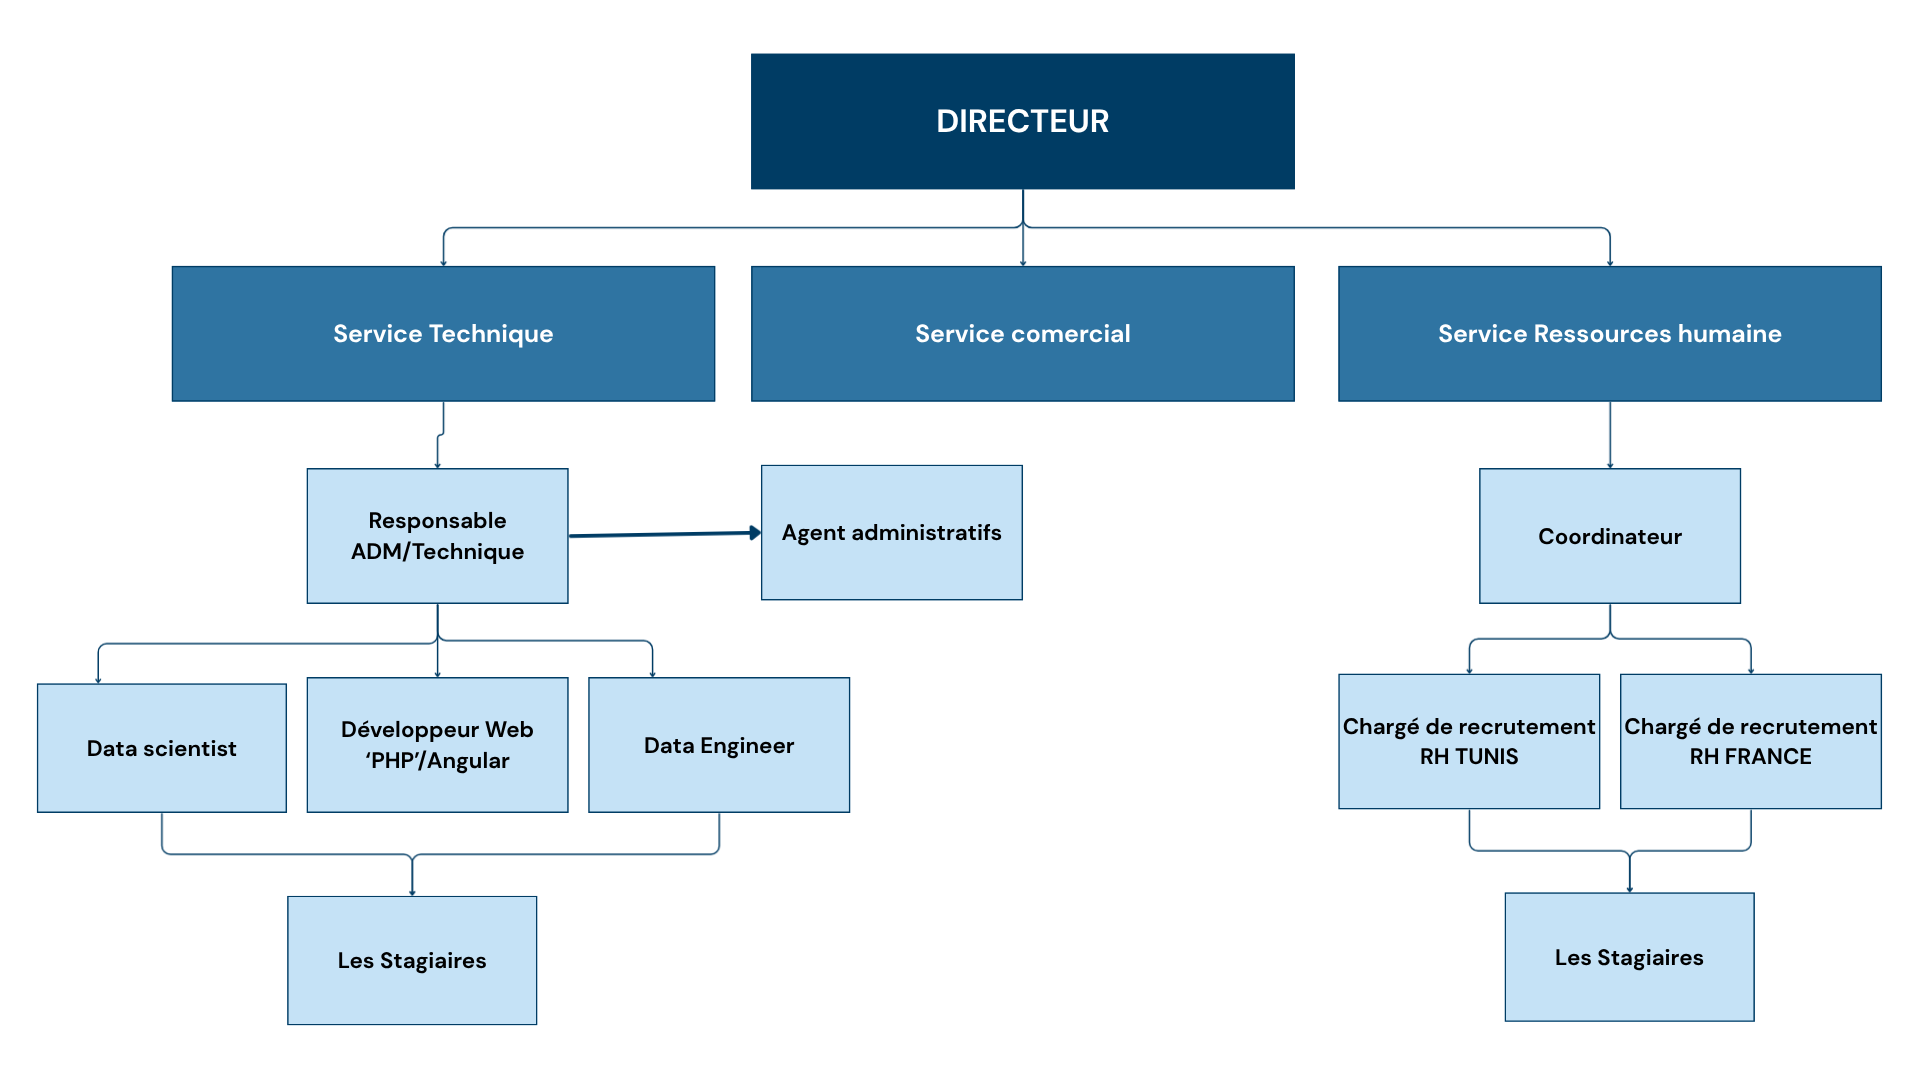
\includegraphics[width=\textwidth]{organigramme.png}
\caption{Organigramme de l'entreprise Smart-Conseil}
\label{fig:organigramme}
\end{figure}

\section{Étude de l'existant}

Le harcèlement scolaire est un phénomène grave et répandu.
Selon la DGESCO (Direction Générale de l'Enseignement Scolaire, service du Ministère de l'Éducation nationale français), environ 800~000 élèves sont victimes de harcèlement scolaire chaque année en France \cite{dgesco2023}.
Avec la généralisation d'Internet, ce phénomène prend désormais une dimension numérique : le cyberharcèlement.
Selon une étude publiée en 2024, 84,7\% des jeunes âgés de 15 à 24 ans passent en moyenne 3h50 par jour en ligne, et 58\% d'entre eux utilisent quotidiennement les réseaux sociaux \cite{digital2024}.

Face à ce problème, plusieurs solutions ont été développées :

\begin{itemize}
    \item Des lignes téléphoniques d'écoute et des questionnaires remplis manuellement par les élèves.
    \item Des outils de signalement intégrés aux plateformes de réseaux sociaux.
    \item \textbf{SafeBar} \cite{safebar} : un outil numérique développé par l'association e-Enfance qui permet de détecter des situations de cyberharcèlement à partir de signalements.
          Il est destiné aux établissements scolaires et aux parents souhaitant surveiller les activités en ligne.
          Il intervient après l'identification d'une victime et ne propose pas de mécanisme de détection préventive.
    \item \textbf{Stop Bashing!} \cite{stopbashing} : une application mobile permettant à un enfant de prendre une capture d'écran d'un message harcelant et de l'envoyer immédiatement à ses parents ou à un adulte référent.
          Le processus de signalement reste entièrement manuel.
    \item \textbf{Netethic} \cite{netethic} : une plateforme numérique développée par Smart-Conseil, dédiée à la détection et à la gestion du harcèlement en milieu scolaire.
          Elle offre un tableau de bord interactif pour visualiser les cas qui demandent l'attention des responsables, un système de gestion et de suivi des signalements, des outils d'analyse et une interface d'administration dédiée aux équipes pédagogiques.
\end{itemize}

\section{Critique de l'existant}

Ces solutions présentent des limites qui laissent plusieurs besoins sans réponse :

\begin{itemize}
    \item \textbf{Disponibilité limitée :} les services d'écoute et de signalement ne sont pas automatisés.
          Les utilisateurs ne peuvent obtenir de l'aide qu'aux heures ouvrées.
    \item \textbf{Barrière psychologique :} une victime peut hésiter à s'adresser directement à un adulte, par crainte des représailles ou de la stigmatisation.
    \item \textbf{Réactivité insuffisante :} un délai important s'écoule entre le signalement et la prise en charge effective de la victime.
    \item \textbf{Absence de support automatisé sur Netethic :} la plateforme ne dispose pas d'un assistant virtuel pour informer les visiteurs extérieurs, ni d'un outil de support automatisé pour le personnel, ni d'un mécanisme de soutien pour les élèves en difficulté, ni d'une analyse automatique des textes soumis.
\end{itemize}

\section{Solution envisagée}

Notre projet s'inscrit dans la plateforme \textbf{Netethic} et a pour objectif d'enrichir cette dernière par quatre modules intelligents et complémentaires basés sur l'intelligence artificielle.
Ces modules répondent directement aux besoins identifiés :

\begin{enumerate}
    \item \textbf{Assistant virtuel public (Noa) :} un assistant conversationnel disponible sur le site de Netethic en français et en anglais, accessible à toute heure, sans intervention humaine.
          Il répond aux questions des visiteurs sur la plateforme, ses fonctionnalités et ses tarifs.
          Il accompagne également les prospects qui souhaitent planifier une démonstration en collectant leurs coordonnées.
          Sa disponibilité continue élimine la dépendance aux horaires du personnel et garantit un accueil permanent des visiteurs.
    \item \textbf{Assistant de support interne :} un assistant destiné au personnel des établissements utilisant Netethic.
          Il répond aux questions sur les fonctionnalités de la plateforme, gère les demandes de rendez-vous et recueille les signalements de dysfonctionnements techniques.
    \item \textbf{Module de soutien émotionnel :} un système qui détecte les signaux de détresse dans les messages des utilisateurs et génère des réponses empathiques adaptées, en orientant l'utilisateur vers les ressources disponibles sur la plateforme.
    \item \textbf{Classificateur de harcèlement :} un système d'analyse automatique des textes qui identifie les types de comportements nécessitant une attention particulière, en s'appuyant sur les références juridiques françaises en vigueur.
\end{enumerate}

\section{Pipeline du projet}

Le projet suit un processus de développement structuré en plusieurs phases :

\begin{enumerate}
    \item \textbf{Phase préalable — Recherche et étude :} recherche bibliographique, analyse des solutions existantes et recueil des besoins auprès des parties prenantes.
    \item \textbf{Collecte et préparation :} recueil des documents de référence (contenu du site Netethic, documentation interne, textes de loi français).
    \item \textbf{Conception :} modélisation de l'architecture générale et des flux de traitement de chaque module.
    \item \textbf{Développement :} implémentation des modules à l'aide de cadres de développement spécialisés en intelligence artificielle.
    \item \textbf{Validation :} tests de performance, évaluation de la qualité des réponses et retours utilisateurs.
\end{enumerate}

\section{Méthodologie}

Pour gérer ce projet, nous avons adopté le cadre Scrum \cite{scrumguide}.
Scrum est une méthode agile de gestion de projet particulièrement adaptée au travail en équipe à distance.
Elle divise le travail en périodes courtes appelées sprints ; chaque sprint dure une semaine et se termine par une révision des résultats obtenus.

\begin{itemize}
    \item \textbf{Daily stand-ups (réunions quotidiennes) :}
          chaque jour, une courte réunion sur Microsoft Teams permet de discuter des objectifs, de l'avancement et des difficultés rencontrées.
    \item \textbf{Sprint Reviews (révisions de sprint) :}
          chaque semaine, une réunion d'équipe permet d'évaluer les tâches réalisées et de planifier le sprint suivant.
\end{itemize}

La modélisation du système a été réalisée avec le langage UML (Unified Modeling Language — langage de modélisation unifié), en utilisant l'outil Power AMC pour la création des diagrammes.

\section*{Conclusion}

Ce chapitre a présenté le cadre général du projet.
Nous avons décrit l'entreprise Smart-Conseil et son domaine d'activité.
Nous avons analysé les solutions existantes face au harcèlement scolaire et mis en évidence leurs limites.
Nous avons ensuite décrit les quatre modules que notre projet apporte à la plateforme Netethic, ainsi que le pipeline de développement et la méthode de gestion adoptés.

Dans le chapitre suivant, nous détaillons la spécification des besoins du système.

\chapter{Spécification des besoins}

\section{Introduction}

Le chapitre précédent a présenté le cadre général du projet au sein de Smart-Conseil,
l'analyse des solutions existantes face au harcèlement scolaire et leurs limites,
ainsi que la solution envisagée composée de quatre modules intelligents.

Ce chapitre définit ce que chaque module doit accomplir.
Il est organisé en cinq parties : les fonctionnalités attendues (besoins fonctionnels),
les contraintes de qualité (besoins non fonctionnels), les acteurs du système,
le diagramme de cas d'utilisation, et l'environnement technique retenu.

% ─────────────────────────────────────────────────────────────────────────────
\section{Identification des besoins fonctionnels}

Les besoins fonctionnels décrivent l'ensemble des fonctionnalités que le système doit
offrir à ses utilisateurs. Ils sont organisés par module.

% ── Module 1 : Noa ────────────────────────────────────────────────────────────
\subsection{Module 1 — Noa : assistant virtuel du site public}

Noa est l'assistant virtuel intégré au site public de Netethic.
Il aide les visiteurs à s'informer sur la plateforme et à planifier une démonstration.
Le Tableau~\ref{tab:bf_noa} présente ses besoins fonctionnels.

\vspace{6pt}
\begin{table}[H]
\caption{Besoins fonctionnels — Noa (assistant site public Netethic)}
\label{tab:bf_noa}
\centering
\small
\setlength{\tabcolsep}{4pt}
\begin{tabular}{|c|p{3.5cm}|p{9.5cm}|}
\hline
\textbf{ID} & \textbf{Besoin} & \textbf{Description} \\
\hline
BF-N01 & Répondre aux questions
        & L'assistant répond aux questions des visiteurs sur les fonctionnalités, les tarifs, le RGPD et les coordonnées de Netethic. \\
\hline
BF-N02 & Gérer la conversation et mémoriser les réponses
        & Le système conserve l'historique des échanges pour maintenir la cohérence de la conversation et retourne instantanément les réponses déjà calculées. \\
\hline
BF-N03 & Classifier l'intention
        & Chaque message est analysé selon son intention — bavardage, question, suivi ou requête interdite — pour lui appliquer le traitement adapté. \\
\hline
BF-N05 & Gérer les bavardages
        & Les salutations, remerciements et messages hors sujet reçoivent des réponses prédéfinies immédiates. \\
\hline
BF-N06 & Appliquer des garde-fous
        & Le système détecte et rejette les requêtes dangereuses ou hors périmètre, comme les tentatives de manipulation ou les demandes de conseils médicaux. \\
\hline
BF-N07 & Gérer les réservations
        & Lorsqu'un visiteur souhaite planifier une démonstration, l'assistant collecte son adresse e-mail et son numéro de téléphone. \\
\hline
BF-N09 & Normaliser les questions
        & Deux questions ayant le même sens partagent la même réponse mémorisée, évitant de recalculer une réponse déjà connue. \\
\hline
BF-N10 & Rechercher dans la base documentaire
        & Pour les questions factuelles, le système recherche les passages les plus pertinents dans la documentation et les intègre dans la réponse. \\
\hline
BF-N12 & Administrer le système
        & L'administrateur peut consulter les statistiques, effacer les réponses mémorisées et accéder aux rendez-vous collectés depuis une interface dédiée. \\
\hline
\end{tabular}
\end{table}

% ── Module 2 : NetEthic Support Assistant ─────────────────────────────────────
\subsection{Module 2 — NetEthic Support Assistant : support technique interne}

Le \textit{NetEthic Support Assistant} est un assistant destiné aux utilisateurs internes de la plateforme.
Il aide le personnel des établissements à utiliser les fonctionnalités de Netethic.
Le Tableau~\ref{tab:bf_nesa} décrit ses besoins fonctionnels.

\vspace{6pt}
\begin{table}[H]
\caption{Besoins fonctionnels — NetEthic Support Assistant (support interne)}
\label{tab:bf_nesa}
\centering
\small
\setlength{\tabcolsep}{4pt}
\begin{tabular}{|c|p{3.5cm}|p{9.5cm}|}
\hline
\textbf{ID} & \textbf{Besoin} & \textbf{Description} \\
\hline
BF-S01 & Filtrer les résultats par catégorie
        & L'utilisateur choisit l'une des 11~catégories de la plateforme avant de poser sa question, ce qui limite la recherche aux documents de ce thème et améliore la précision des réponses. \\
\hline
BF-S03 & Mise en mémoire des réponses
        & Les réponses générées sont mémorisées. Pour les questions ultérieures similaires, la réponse est retournée directement sans solliciter le modèle. \\
\hline
BF-S04 & Gestion de session
        & Chaque session utilisateur est conservée 24~heures avec l'historique de conversation et les informations d'identité (nom, e-mail, téléphone). \\
\hline
BF-S05 & Questions suggérées
        & Plus de 60~questions prédéfinies sont proposées à l'utilisateur pour l'aider à explorer les fonctionnalités de la plateforme. \\
\hline
BF-S06 & Données en temps réel
        & En mode \textit{Insights}, l'assistant répond aux questions sur les données du tableau de bord (toxicité, profils à risque, climat scolaire, tendances) transmises par la plateforme à l'ouverture de la session. \\
\hline
BF-S07 & Génération automatique de description
        & Avant l'affichage d'un formulaire de rendez-vous ou de signalement, l'assistant rédige automatiquement un motif ou une description à partir de la conversation. Ce texte pré-remplit le formulaire et reste modifiable. \\
\hline
BF-S08 & Analytique d'usage
        & Le système enregistre chaque question avec son thème et les éventuels déclenchements de sécurité pour permettre l'amélioration continue de la documentation. \\
\hline
BF-S09 & Prise de rendez-vous
        & Lorsque la documentation ne permet pas de répondre, l'assistant propose de planifier un rendez-vous de support sans que l'utilisateur ait à ressaisir ses informations. \\
\hline
BF-S10 & Signalement de dysfonctionnements
        & L'utilisateur peut signaler un incident via un formulaire pré-rempli automatiquement. Le rapport est ensuite transmis à l'équipe technique de Netethic. \\
\hline
BF-S11 & Accès au portail de support
        & Lorsqu'aucune réponse documentaire n'est trouvée, l'utilisateur peut accéder directement au portail de support en ligne. \\
\hline
BF-S12 & Détection des questions de suivi
        & Le système détecte si une question fait suite au sujet précédent et, le cas échéant, réutilise les résultats de recherche déjà obtenus pour répondre de façon cohérente. \\
\hline
\end{tabular}
\end{table}

% ── Module 3 : Soutien émotionnel ─────────────────────────────────────────────
\subsection{Module 3 — Module de soutien émotionnel}

Ce module détecte les signaux de détresse psychologique dans les messages des utilisateurs.
Il y répond avec empathie et oriente vers les ressources disponibles.
Le Tableau~\ref{tab:bf_emo} décrit ses besoins fonctionnels.

\vspace{6pt}
\begin{table}[H]
\caption{Besoins fonctionnels — Module de soutien émotionnel}
\label{tab:bf_emo}
\centering
\small
\setlength{\tabcolsep}{4pt}
\begin{tabular}{|c|p{3.5cm}|p{9.5cm}|}
\hline
\textbf{ID} & \textbf{Besoin} & \textbf{Description} \\
\hline
BF-E01 & Détecter la détresse
        & Le système détecte six types de signaux de détresse dans les messages : dépression, idéation suicidaire, solitude, anxiété, colère et comportements addictifs. \\
\hline
BF-E02 & Alerte urgente
        & En cas d'idéation suicidaire, une réponse d'urgence est générée immédiatement avec les numéros d'aide (urgences, cyberviolences, CNAE), toujours présents quelle que soit la réponse générée. \\
\hline
BF-E03 & Répondre avec empathie
        & Pour les signaux non urgents, l'assistant génère une réponse chaleureuse et empathique, adaptée au type de détresse et à la langue de l'utilisateur. \\
\hline
BF-E04 & Orienter vers l'accompagnement
        & Après détection d'un signal de détresse, le module oriente l'utilisateur vers le module \textit{Accompagnement} de Netethic pour un suivi par un professionnel. \\
\hline
BF-E05 & Journaliser les événements
        & Chaque détection est enregistrée avec son type et son horodatage, sans conserver le contenu du message, dans le respect de la confidentialité. \\
\hline
BF-E06 & Mémoriser le profil utilisateur
        & L'assistant mémorise les informations révélées au fil des échanges (prénom, sources de stress, situation scolaire) dans un profil persistant de 30~jours pour personnaliser les réponses lors des sessions suivantes. \\
\hline
BF-E07 & Limiter le débit des messages
        & Le nombre de messages envoyés par utilisateur est limité sur une courte période afin de protéger le service contre les abus. \\
\hline
BF-E08 & Prendre en charge l'arabe et le darija
        & En plus du français et de l'anglais, le module prend en charge l'arabe et le darija tunisien. L'assistant répond toujours dans la langue de l'utilisateur, sans mélange ni traduction. \\
\hline
\end{tabular}
\end{table}

% ── Module 4 : Classificateur de harcèlement ──────────────────────────────────
\subsection{Module 4 — Classificateur de harcèlement}

Ce module analyse automatiquement les textes soumis à la plateforme.
Il identifie les comportements nécessitant une attention particulière et s'appuie sur le droit français.
Le Tableau~\ref{tab:bf_class} détaille ses besoins fonctionnels.

\vspace{6pt}
\begin{table}[H]
\caption{Besoins fonctionnels — Classificateur de harcèlement}
\label{tab:bf_class}
\centering
\small
\setlength{\tabcolsep}{4pt}
\begin{tabular}{|c|p{3.5cm}|p{9.5cm}|}
\hline
\textbf{ID} & \textbf{Besoin} & \textbf{Description} \\
\hline
BF-C01 & Classification multi-méthodes
        & Le système compare quatre stratégies : inférence LLM seul, avec ancrage juridique, heuristiques par mots-clés, et approche hybride avec repli automatique. \\
\hline
BF-C02 & Taxonomie à 16 catégories
        & Chaque texte reçoit plusieurs étiquettes simultanées : 10 actes de harcèlement (Groupe A) et 6 signaux de détresse (Groupe B). \\
\hline
BF-C03 & Ancrage sur textes juridiques
        & Les documents légaux français (Loi 2022 \cite{sparkloi}, Code pénal) sont indexés et intégrés dans l'analyse pour ancrer les décisions dans le cadre légal. \\
\hline
BF-C04 & Prétraitement du texte
        & Avant classification, chaque texte est normalisé : suppression des URLs, normalisation des espaces et mise en minuscules. \\
\hline
BF-C05 & Chaîne de repli
        & En cas d'échec du modèle principal, le système bascule sur les heuristiques, puis sur une étiquette neutre, garantissant toujours une réponse. \\
\hline
BF-C06 & Alerte urgente
        & Une idéation suicidaire détectée active un indicateur d'urgence dans la sortie pour déclencher une prise en charge prioritaire. \\
\hline
BF-C07 & Journalisation des résultats
        & Chaque classification est enregistrée avec son horodatage, sa stratégie, son niveau de confiance et sa latence. \\
\hline
BF-C08 & Suivi des expériences
        & Le système peut récupérer et retraiter les données d'expériences passées pour comparer et améliorer les méthodes. \\
\hline
BF-C09 & Traitement en parallèle
        & Le pipeline traite plusieurs textes simultanément et calcule des métriques d'évaluation agrégées sur l'ensemble des méthodes. \\
\hline
\end{tabular}
\end{table}

% ─────────────────────────────────────────────────────────────────────────────
\section{Identification des besoins non fonctionnels}

Les besoins non fonctionnels définissent les contraintes de qualité que l'ensemble du
système doit respecter. Le Tableau~\ref{tab:besoins_non_fonctionnels} présente ces exigences.

\vspace{6pt}
\begin{table}[H]
\caption{Besoins non fonctionnels du système global}
\label{tab:besoins_non_fonctionnels}
\centering
\small
\setlength{\tabcolsep}{4pt}
\begin{tabular}{|c|p{3cm}|p{9.8cm}|}
\hline
\textbf{ID} & \textbf{Catégorie} & \textbf{Description} \\
\hline
BNF-01 & Performance
        & Le temps de réponse est inférieur à 1~ms pour les questions mémorisées et inférieur à 5~secondes pour un traitement complet. \\
\hline
BNF-02 & Sécurité
        & Les clés de connexion ne sont jamais exposées côté navigateur, les communications sensibles transitent via HTTPS et les requêtes malveillantes sont filtrées. \\
\hline
BNF-03 & Disponibilité
        & Les services sont accessibles 24h/24 et 7j/7, avec des mécanismes de repli en cas d'indisponibilité du modèle externe. \\
\hline
BNF-04 & Scalabilité
        & Tous les composants sont conteneurisés via Docker \cite{docker}, permettant le déploiement de plusieurs instances selon la charge. \\
\hline
BNF-05 & Maintenabilité
        & L'architecture modulaire isole chaque fonctionnalité dans un module distinct, facilitant les mises à jour et les corrections. \\
\hline
BNF-06 & Conformité RGPD
        & Aucune donnée personnelle n'est conservée au-delà de la session ; les données de réservation sont stockées localement sans partage avec des tiers. \\
\hline
BNF-07 & Multilingue
        & L'interface et les réponses sont disponibles en français, en anglais et en arabe, avec détection automatique de la langue. Le module de soutien émotionnel étend ce support au darija tunisien et au code-switching arabo-français. \\
\hline
BNF-08 & Robustesse
        & Chaque composant intègre une gestion explicite des erreurs avec des messages clairs pour l'utilisateur et des traces journalisées côté serveur. \\
\hline
\end{tabular}
\end{table}

% ─────────────────────────────────────────────────────────────────────────────
\section{Identification des acteurs}

Un acteur représente toute entité externe qui interagit avec le système.
Sept acteurs principaux sont identifiés.
Conformément aux consignes de l'ISTIC, les assistants virtuels sont représentés
comme des acteurs à part entière avec le stéréotype \textit{«Actor»}.

\subsection{Visiteur du site public}

Le visiteur est toute personne qui accède au site web de Netethic.
Il peut s'agir d'un directeur d'établissement scolaire, d'un conseiller principal d'éducation,
d'un parent ou d'un représentant d'association.
Il interagit avec Noa pour s'informer sur la plateforme, poser des questions en français
ou en anglais, et réserver une démonstration.

\subsection{Utilisateur interne de la plateforme}

L'utilisateur interne est un membre du personnel d'un établissement disposant
d'un accès authentifié à la plateforme Netethic.
Il interagit avec le \textit{NetEthic Support Assistant} pour obtenir de l'aide sur
les fonctionnalités de la plateforme, déclarer un incident technique ou planifier
un rendez-vous de support.

\subsection{Administrateur}

L'administrateur est le responsable technique du système.
Il surveille l'état des caches, consulte les statistiques d'usage, gère les sessions actives
et accède aux rendez-vous collectés et aux signalements reçus.

\subsection{Noa et NetEthic Support Assistant (stéréotype «Actor»)}

Noa et le \textit{NetEthic Support Assistant} sont les deux assistants virtuels du système.
Conformément aux consignes de l'ISTIC pour les projets intégrant un module d'IA générative,
ils sont représentés dans le diagramme de cas d'utilisation avec le stéréotype \textit{«Actor»}.
Chacun orchestre de manière autonome son pipeline de traitement.

\subsection{Module de soutien émotionnel (stéréotype «Actor»)}

Le module de soutien émotionnel est un composant intelligent de la plateforme Netethic.
Il détecte les signaux de détresse dans les messages des utilisateurs, génère des réponses
empathiques et déclenche les alertes en cas de crise.
Il est représenté comme un acteur avec le stéréotype \textit{«Actor»} car il orchestre
de manière autonome son pipeline de traitement.

\subsection{Classificateur de harcèlement (stéréotype «Actor»)}

Le classificateur de harcèlement est un module d'analyse automatique de textes soumis
par la plateforme Netethic.
Il identifie les comportements problématiques, les signaux de harcèlement et ancre ses
décisions dans le cadre juridique français.
Il est représenté comme un acteur avec le stéréotype \textit{«Actor»} car il conduit
de manière autonome son pipeline d'analyse.

\subsection{Serveur LLM (kaisens.fr)}

Un LLM (Large Language Model — grand modèle de langage) est un modèle entraîné sur de grandes
quantités de texte, capable de générer des réponses en langage naturel et de suivre des instructions.
Le serveur LLM est un serveur d'inférence externe hébergé sur l'infrastructure de kaisens.fr \cite{vllm2023}.
Il expose une interface compatible avec les standards de l'industrie et génère les réponses
à partir du modèle Mistral-7B \cite{mistral2023}.
Il est sollicité par les deux assistants virtuels ainsi que par le classificateur de harcèlement.

% ─────────────────────────────────────────────────────────────────────────────
\section{Diagramme de cas d'utilisation}

Le diagramme de cas d'utilisation illustre les interactions entre les acteurs du système
et les fonctionnalités disponibles.
Conformément aux consignes spécifiques aux projets intégrant un module d'IA générative,
les assistants Noa et NetEthic Support Assistant sont représentés comme des acteurs
portant le stéréotype \textit{«Actor»}.

La Figure~\ref{fig:use_case} illustre le système global.
Le visiteur est l'acteur principal de Noa : il initie les conversations, pose des questions
sur la plateforme et réserve une démonstration.
L'utilisateur interne est l'acteur principal du \textit{NetEthic Support Assistant} :
il pose des questions, signale des incidents et peut bénéficier du soutien émotionnel.
L'administrateur supervise les deux systèmes.
Le serveur LLM externe fournit la capacité de génération à l'ensemble des modules.

\begin{figure}[H]
\centering
% \includegraphics[width=0.95\textwidth]{use_case_global.png}
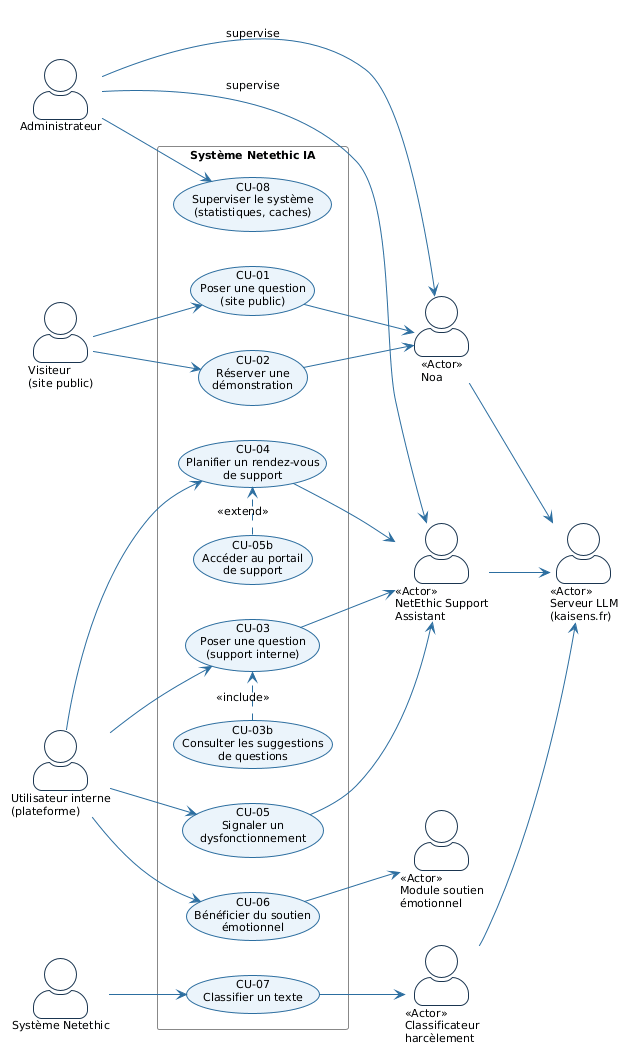
\includegraphics[width=0.95\textwidth]{figures_png/01_use_case_global.png}
\caption{Diagramme de cas d'utilisation global du système}
\label{fig:use_case}
\end{figure}

Le Tableau~\ref{tab:cas_utilisation} décrit les cas d'utilisation essentiels du système.

\vspace{6pt}
\begin{table}[H]
\caption{Description des cas d'utilisation essentiels}
\label{tab:cas_utilisation}
\centering
\small
\setlength{\tabcolsep}{3pt}
\begin{tabular}{|c|p{3cm}|p{2.8cm}|p{7.2cm}|}
\hline
\textbf{ID} & \textbf{Cas d'utilisation} & \textbf{Acteur principal} & \textbf{Description} \\
\hline
CU-01 & Poser une question (site public)
       & Visiteur
       & Le visiteur pose une question en français ou en anglais.
         Noa la traite selon son pipeline : classification, mémoire, recherche, génération. \\
\hline
CU-02 & Réserver une démonstration
       & Visiteur
       & Le visiteur exprime le souhait de planifier une démo.
         L'agent conversationnel collecte son e-mail et son téléphone. \\
\hline
CU-03 & Poser une question (support interne)
       & Utilisateur interne
       & L'utilisateur sélectionne une catégorie parmi les 11~modules, puis pose sa question.
         Le Support Assistant retourne une réponse ancrée dans la documentation. \\
\hline
CU-03b & Consulter les suggestions de questions
        & Utilisateur interne
        & Inclus dans CU-03. L'assistant propose plus de 60~questions prédéfinies réparties
          sur les 11~catégories pour guider l'utilisateur dans l'exploration des fonctionnalités. \\
\hline
CU-04 & Planifier un rendez-vous de support
       & Utilisateur interne
       & Si la documentation ne permet pas de répondre, l'assistant propose un rendez-vous
         et collecte les informations nécessaires. \\
\hline
CU-05 & Signaler un dysfonctionnement
       & Utilisateur interne
       & L'utilisateur déclenche le formulaire de signalement. L'assistant collecte
         les informations et transmet le rapport. \\
\hline
CU-05b & Accéder au portail de support
        & Utilisateur interne
        & Étend CU-04. Lorsqu'aucune documentation ne répond à la question, l'utilisateur
          peut accéder directement au portail de support en ligne pour consulter les
          ressources additionnelles ou contacter l'équipe. \\
\hline
CU-06 & Bénéficier du soutien émotionnel
       & Utilisateur interne
       & Si un signal de détresse est détecté, le module génère une réponse empathique
         et oriente vers le module Accompagnement. En cas d'idéation suicidaire, une alerte est déclenchée. \\
\hline
CU-07 & Classifier un texte
       & Système Netethic
       & La plateforme soumet un texte. Le classificateur retourne les étiquettes détectées,
         le niveau de confiance et un indicateur d'urgence si nécessaire. \\
\hline
CU-08 & Superviser le système
       & Administrateur
       & L'administrateur consulte les statistiques, les rendez-vous collectés,
         les signalements et l'état des caches. \\
\hline
\end{tabular}
\end{table}

% ─────────────────────────────────────────────────────────────────────────────
\section{Identification des besoins techniques}

Cette section décrit l'environnement matériel et logiciel utilisé pour le développement du projet.

\subsection{Environnement de travail}

Le Tableau~\ref{tab:env_travail} présente les équipements et outils utilisés lors du développement.

\vspace{6pt}
\begin{table}[H]
\caption{Environnement de travail}
\label{tab:env_travail}
\centering
\small
\setlength{\tabcolsep}{4pt}
\begin{tabular}{|p{4cm}|p{10.5cm}|}
\hline
\textbf{Composant} & \textbf{Description} \\
\hline
Système d'exploitation & Windows 11 Home (version 10.0.26200) \\
\hline
Environnement de développement & Visual Studio Code avec extensions Python, Scala et Docker \\
\hline
Gestion de version    & Git / GitLab (dépôt : \texttt{gitlab.dataforethic.fr}) \\
\hline
Conteneurisation      & Docker Desktop (Docker Compose v2) \cite{docker} \\
\hline
Gestion de projet     & Méthode Scrum \cite{scrumguide} — réunions hebdomadaires sur Microsoft Teams \\
\hline
Modélisation UML      & Power AMC \\
\hline
\end{tabular}
\end{table}

\subsection{Environnement logiciel}

Le Tableau~\ref{tab:env_logiciel} présente la pile logicielle utilisée.
Les choix technologiques ont été guidés par des critères d'efficacité, d'ouverture
et d'adéquation avec les exigences de chaque module.

\vspace{6pt}
\begin{table}[H]
\caption{Environnement logiciel global}
\label{tab:env_logiciel}
\centering
\small
\setlength{\tabcolsep}{3pt}
\begin{tabular}{|p{2.5cm}|p{4.5cm}|p{1.8cm}|p{5.5cm}|}
\hline
\textbf{Couche} & \textbf{Technologie} & \textbf{Version} & \textbf{Rôle} \\
\hline
Backend Python  & Python               & 3.11             & Langage principal — modules Noa et Support Assistant \\
\hline
Backend Python  & FastAPI \cite{fastapi} & $\geq$ 0.110   & Framework web — expose les interfaces de programmation REST \\
\hline
Backend Scala   & Scala                & 2.12.18          & Langage principal — module classificateur \\
\hline
Backend Scala   & Apache Spark         & 3.5.0            & Moteur de traitement de données à grande échelle \\
\hline
Orchestration   & LangChain \cite{langchain} & $\geq$ 0.2.0 & Orchestration des étapes de traitement conversationnel \\
\hline
Représentation sémantique & sentence-transformers \cite{sbert} & $\geq$ 2.7.0 & Calcul des vecteurs de représentation sémantique \\
\hline
Base documentaire & ChromaDB \cite{chromadb} & $\geq$ 0.5    & Stockage et recherche documentaire par similarité \\
\hline
Serveur LLM     & vLLM — kaisens.fr \cite{vllm2023} & —       & Serveur d'inférence externe, compatible API OpenAI \\
\hline
Modèle LLM      & Mistral-7B-Instruct \cite{mistral2023} & —   & Modèle de génération et de classification de texte \\
\hline
Sessions / Cache & Redis \cite{redis}  & $\geq$ 5.0       & Historique conversationnel et mémoire des réponses \\
\hline
Interface Noa   & React + Vite         & 18 / 5           & Interface chatbot — site public \\
\hline
Interface Support & Streamlit          & $\geq$ 1.32.0    & Interface assistant support interne \\
\hline
Déploiement     & Docker Compose \cite{docker} & —          & Conteneurisation et orchestration des services \\
\hline
\end{tabular}
\end{table}

% ─────────────────────────────────────────────────────────────────────────────
\section{Conclusion}

Ce chapitre a défini les besoins du système dans sa globalité.
Les besoins fonctionnels ont établi les fonctionnalités attendues de chacun des quatre modules.
Les besoins non fonctionnels ont précisé les contraintes de qualité transversales,
notamment en matière de performance, de sécurité, de disponibilité et de conformité RGPD.
Les sept acteurs du système ont été identifiés, avec une représentation particulière
des assistants virtuels et des modules autonomes en tant qu'acteurs à stéréotype \textit{«Actor»}.
Le diagramme de cas d'utilisation a synthétisé l'ensemble de ces interactions.

Dans le chapitre suivant, nous présentons l'état de l'art et les choix technologiques
retenus pour chacun des quatre modules.

\chapter{État de l'art et choix technologiques}
\markboth{Chapitre 2}{}

\section*{Introduction}

Le chapitre précédent a présenté le cadre du projet, analysé les solutions existantes
et défini les besoins fonctionnels et non fonctionnels des quatre modules.
Ce chapitre présente une étude des approches existantes dans les domaines couverts par le projet,
et justifie les choix technologiques retenus pour chacun des quatre modules.
Il est organisé en six axes : les assistants conversationnels,
la recherche documentaire intelligente, les modèles de génération de langage,
l'assistant émotionnel par intelligence artificielle,
la détection automatique du harcèlement,
et l'orchestration des pipelines conversationnels.
Chaque axe se conclut par une justification du choix retenu.

% ─────────────────────────────────────────────────────────────────────────────
\section{Assistants conversationnels}

\subsection{Évolution des approches}

Un assistant conversationnel est un programme capable de tenir une conversation
avec un utilisateur humain en langage naturel.
Ces systèmes ont évolué en plusieurs générations successives.

\textbf{Chatbots à règles.}
Les premiers systèmes reposaient sur des règles explicites du type
« si l'utilisateur dit X, répondre Y ».
Le programme fondateur est \textit{ELIZA}, créé en 1966 \cite{eliza1966}.
Ces systèmes sont rapides et prévisibles, mais incapables de traiter
des formulations non anticipées.

\textbf{Chatbots à intentions.}
À partir des années 2010, des plateformes comme Dialogflow \cite{dialogflow} ont introduit
la classification d'intention à partir d'exemples d'entraînement.
Ces systèmes sont plus souples, mais restent limités aux catégories définies
à l'avance et nécessitent un travail d'annotation important.

\textbf{Chatbots à grand modèle de langage.}
Les LLMs génèrent des réponses en langage naturel sans entraînement spécifique, mais peuvent produire des informations incorrectes — phénomène appelé \textit{hallucination}.

\textbf{Génération ancrée dans la documentation (RAG).}
L'architecture RAG (Retrieval-Augmented Generation — génération augmentée
par récupération) combine un LLM et une base de connaissances \cite{lewis2020rag}.
Le modèle répond uniquement à partir des documents fournis,
ce qui réduit significativement les hallucinations
et permet de contrôler le périmètre des réponses.

\subsection{Tableau comparatif}

Le Tableau~\ref{tab:comparatif_chatbots} compare les quatre approches
selon les critères pertinents pour le projet.

\vspace{6pt}
\begin{table}[H]
\centering
\caption{Comparaison des approches pour les assistants conversationnels}
\label{tab:comparatif_chatbots}
\begin{tabular}{|l|c|c|c|c|}
\hline
\textbf{Critère} & \textbf{Règles} & \textbf{Intentions} & \textbf{LLM seul} & \textbf{RAG} \\
\hline
Flexibilité & Faible & Moyenne & Élevée & Élevée \\
Fiabilité des réponses & Élevée & Moyenne & Faible & Élevée \\
Contrôle du périmètre & Élevé & Élevé & Faible & Élevé \\
Besoin de données & Aucun & Moyen & Aucun & Documents \\
Mise à jour facile & Non & Non & Non & Oui \\
\hline
\end{tabular}
\end{table}

\subsection{Choix retenu}

L'architecture RAG a été retenue pour les modules Noa assistant et assistant technique.
Elle combine la flexibilité d'un LLM avec la fiabilité d'une base documentaire maîtrisée,
ce qui est indispensable dans un contexte où les réponses incorrectes
peuvent avoir des conséquences sur des situations sensibles.
L'assistant émotionnel, en revanche, ne dispose pas de base documentaire fixe :
il repose sur un LLM en mode conversationnel pur, dont le comportement
est adapté à chaque échange selon le profil et l'état émotionnel de l'utilisateur.

% ─────────────────────────────────────────────────────────────────────────────
\section{Recherche documentaire intelligente}

\subsection{Approches existantes}

La recherche documentaire consiste à retrouver, parmi un ensemble de documents,
les passages les plus pertinents pour répondre à une question donnée.

\textbf{Recherche par mots-clés (TF-IDF).}
La méthode classique repose sur la fréquence des mots dans les documents.
Elle est rapide mais insensible au sens : une question formulée différemment
ne retrouvera pas les mêmes documents, même s'ils traitent du même sujet.

\textbf{Recherche par similarité sémantique.}
Les modèles d'encodage modernes transforment chaque texte
en un vecteur numérique \cite{sbert}.
Deux textes au sens similaire produisent des vecteurs proches,
mesurés par la similarité cosinus.
Cette approche est robuste aux reformulations et aux synonymes.

\textbf{Bases de données vectorielles.}
Les vecteurs générés sont indexés dans des bases spécialisées
qui permettent une recherche efficace parmi des milliers de documents.
Plusieurs solutions existent : Pinecone (hébergée dans le cloud),
FAISS (bibliothèque locale non persistante),
et ChromaDB (base locale persistante et légère).

\subsection{Choix retenus}

Le modèle d'encodage retenu est \texttt{paraphrase-multilingual-mpnet-base-v2} \cite{sbert},
pour sa compatibilité française et anglaise, sa robustesse aux reformulations
et son fonctionnement sans processeur graphique dédié.
La base vectorielle retenue est \textbf{ChromaDB} \cite{chromadb},
pour sa persistance locale, sa légèreté et son intégration aisée dans les pipelines Python.

% ─────────────────────────────────────────────────────────────────────────────
\section{Modèles de génération de langage}

\subsection{Panorama des modèles disponibles}

Plusieurs modèles de génération de langage sont disponibles pour des projets
nécessitant une inférence locale ou une maîtrise des données.

\textbf{GPT-4 (OpenAI).}
Modèle très performant, accessible via API.
Son utilisation implique que les données sont envoyées à des serveurs externes,
ce qui pose des problèmes de confidentialité dans le contexte scolaire.

\textbf{LLaMA (Meta).}
Famille de modèles ouverts utilisables localement.
Performants mais moins bien adaptés au français.

\textbf{Mistral (Mistral AI).}
Modèles développés par une entreprise française, disponibles en open source.
Le modèle \textbf{Mistral-7B-Instruct} \cite{mistral2023} est optimisé
pour suivre des instructions et offre un excellent rapport performance/ressources
pour la langue française.

\subsection{Tableau comparatif}

Le Tableau~\ref{tab:comparatif_llm} compare les principaux modèles
selon les critères du projet.

\vspace{6pt}
\begin{table}[H]
\centering
\caption{Comparaison des modèles de génération de langage}
\label{tab:comparatif_llm}
\begin{tabular}{|l|c|c|c|}
\hline
\textbf{Critère} & \textbf{GPT-4} & \textbf{LLaMA} & \textbf{Mistral-7B} \\
\hline
Hébergement local & Non & Oui & Oui \\
Qualité en français & Élevée & Moyenne & Élevée \\
Ressources requises & Cloud & Élevées & Modérées \\
Licence ouverte & Non & Oui & Oui \\
Confidentialité des données & Non & Oui & Oui \\
\hline
\end{tabular}
\end{table}

\subsection{Choix retenu}

Le modèle \textbf{Mistral-7B-Instruct} a été retenu pour sa qualité en français,
son hébergement local (garantissant la confidentialité des données des élèves),
et son accessibilité via le serveur LLM kaisens.fr.
La version AWQ, une version compressée du modèle, est utilisée
pour réduire les ressources mémoire sans perte significative de qualité.
Le serveur d'inférence \textbf{vLLM} \cite{vllm2023} permet de traiter
plusieurs requêtes simultanément.
Ce serveur est déjà déployé et opérationnel sur l'infrastructure de kaisens.fr,
ce qui élimine tout coût d'infrastructure supplémentaire et permet une intégration
immédiate sans mise en place d'un environnement GPU dédié.

% ─────────────────────────────────────────────────────────────────────────────
\section{assistant émotionnel par intelligence artificielle}

\subsection{Approches existantes}

L'assistant émotionnel automatisé vise à détecter les signaux de détresse
dans les messages d'un utilisateur et à générer des réponses empathiques adaptées.
Plusieurs approches ont été explorées dans la littérature et les applications commerciales.

\textbf{Scripts prédéfinis (chatbots guidés).}
Des applications comme Woebot ou Wysa reposent sur des arbres de décision
et des scripts thérapeutiques prédéfinis inspirés des techniques cognitivo-comportementales.
Ces systèmes sont prévisibles et sûrs, mais rigides :
ils ne peuvent pas s'adapter à une conversation libre
et offrent une expérience répétitive à long terme.

\textbf{Détection par mots-clés.}
Une approche simple consiste à rechercher des mots ou expressions
associés à une situation de crise (mal-être, idées suicidaires, violence).
Elle est rapide mais produit de nombreuses fausses alertes
et ne capture pas le contexte ni la nuance d'un message.

\textbf{Classifieurs d'apprentissage automatique.}
Des modèles supervisés entraînés sur des corpus annotés
permettent une détection plus fine de la détresse émotionnelle.
Ces modèles se concentrent sur la classification et ne génèrent pas de réponse empathique ;
ils nécessitent par ailleurs un corpus étiqueté conséquent, difficile à constituer.

\textbf{LLM conversationnel avec profil utilisateur.}
Un grand modèle de langage utilisé en mode conversationnel peut à la fois
détecter la détresse et générer une réponse empathique adaptée au contexte.
L'ajout d'un profil utilisateur persistant, mis à jour au fil des sessions,
permet au système de personnaliser les réponses en tenant compte
de la situation propre à chaque élève.

\subsection{Tableau comparatif}

Le Tableau~\ref{tab:comparatif_emotionnel} compare ces approches
selon les critères pertinents pour l'assistant émotionnel.

\vspace{6pt}
\begin{table}[H]
\centering
\caption{Comparaison des approches pour l'assistant émotionnel}
\label{tab:comparatif_emotionnel}
\begin{tabular}{|l|c|c|c|c|}
\hline
\textbf{Critère} & \textbf{Scripts} & \textbf{Mots-clés} & \textbf{ML supervisé} & \textbf{LLM conversationnel} \\
\hline
Flexibilité & Faible & Faible & Moyenne & Élevée \\
Qualité empathique & Moyenne & Nulle & Nulle & Élevée \\
Données d'entraînement & Aucune & Aucune & Élevées & Aucune \\
Personnalisation & Non & Non & Non & Oui \\
Détection de détresse & Manuelle & Partielle & Oui & Oui \\
\hline
\end{tabular}
\end{table}

\subsection{Choix retenu}

L'approche retenue est le \textbf{LLM conversationnel avec profil utilisateur persistant}.
Contrairement aux modules Noa assistant et assistant technique,
ce module n'a pas de base documentaire à consulter :
les réponses doivent s'adapter à l'état émotionnel de l'utilisateur,
pas à un corpus de documents.
Un profil est extrait automatiquement de la conversation et enrichi à chaque session,
permettant des réponses de plus en plus personnalisées.
Des garde-fous basés sur la classification du contenu détectent
les situations de crise et déclenchent une réponse adaptée
avec les numéros d'urgence appropriés.

% ─────────────────────────────────────────────────────────────────────────────
\section{Détection automatique du harcèlement}

\subsection{Approches existantes}

La détection automatique du harcèlement dans les textes est un problème
activement étudié en traitement automatique du langage naturel.

\textbf{Listes de mots offensants.}
L'approche la plus simple consiste à rechercher des mots ou expressions
préalablement identifiés comme offensants.
Elle est rapide mais incapable de saisir le contexte, l'ironie ou l'argot.

\textbf{Modèles d'apprentissage automatique classiques.}
Des modèles comme la régression logistique ou les SVM permettent
une classification binaire à partir de caractéristiques textuelles.
Ils nécessitent des données d'entraînement étiquetées et restent limités
pour les taxonomies complexes à plusieurs catégories.

\textbf{Modèles de type BERT.}
Les modèles basés sur l'architecture Transformer (comme CamemBERT pour le français)
offrent une meilleure compréhension du contexte.
Ils nécessitent un corpus d'entraînement étiqueté conséquent,
difficile à constituer dans le domaine du harcèlement scolaire en français.

\textbf{Génération ancrée dans des textes juridiques.}
Une approche originale consiste à guider le modèle de génération
par les textes de loi pertinents \cite{sparkloi}.
La décision est ainsi ancrée dans le droit français,
ce qui renforce la légitimité des résultats dans un contexte légal encadré.

\subsection{Tableau comparatif}

Le Tableau~\ref{tab:comparatif_classif} compare ces approches selon les critères du projet.

\vspace{6pt}
\begin{table}[H]
\centering
\caption{Comparaison des approches de détection du harcèlement}
\label{tab:comparatif_classif}
\begin{tabular}{|l|c|c|c|c|}
\hline
\textbf{Critère} & \textbf{Mots-clés} & \textbf{ML classique} & \textbf{BERT} & \textbf{RAG juridique} \\
\hline
Données d'entraînement & Aucune & Élevées & Élevées & Aucune \\
Compréhension du contexte & Faible & Moyenne & Élevée & Élevée \\
Taxonomie complexe & Non & Non & Partielle & Oui \\
Ancrage légal & Non & Non & Non & Oui \\
Mise à jour facile & Oui & Non & Non & Oui \\
\hline
\end{tabular}
\end{table}

\subsection{Choix retenu}

L'approche retenue est la \textbf{génération ancrée dans des textes juridiques},
combinée à un mécanisme de repli sur des règles heuristiques.
Cette combinaison offre à la fois la richesse sémantique d'un LLM
et la solidité d'un ancrage légal, sans nécessiter de corpus étiqueté.
Elle est implémentée en quatre stratégies comparées en parallèle,
détaillées dans le chapitre suivant.

% ─────────────────────────────────────────────────────────────────────────────
\section{Orchestration des pipelines conversationnels}

Les modules conversationnels du projet (Noa assistant, assistant technique, assistant émotionnel)
nécessitent une couche d'orchestration capable de chaîner plusieurs opérations :
classification d'intention, recherche documentaire, appel au modèle de langage
et gestion de la mémoire de session.
Plusieurs frameworks ont été étudiés pour remplir ce rôle.

\subsection{Frameworks disponibles}

\textbf{Implémentation personnalisée.}
Il est possible de gérer manuellement l'enchaînement des appels API
(ChromaDB, vLLM, Redis) sans framework dédié.
Cette approche offre un contrôle total mais impose un effort de développement
important pour chaque nouvelle fonctionnalité, sans bénéficier des abstractions
et optimisations déjà disponibles dans les outils spécialisés.

\textbf{LlamaIndex.}
LlamaIndex est un framework centré sur l'indexation et la recherche documentaire.
Il propose des connecteurs vers de nombreuses sources de données
et simplifie la construction de pipelines RAG.
Cependant, son périmètre est plus étroit que celui de LangChain :
il couvre moins bien la gestion de la mémoire conversationnelle,
les agents à boucle d'outils et l'orchestration de flux multi-étapes.

\textbf{LangChain.}
LangChain \cite{langchain} est un framework open source conçu spécifiquement
pour les applications fondées sur des modèles de langage.
Il fournit des abstractions pour les chaînes de traitement (\textit{chains}),
les agents (\textit{tool-use}), la mémoire conversationnelle, les connecteurs
vers les bases vectorielles et les modèles de langage.
Il supporte nativement ChromaDB, Redis et les API compatibles OpenAI,
ce qui correspond exactement à la pile technologique retenue pour ce projet.

\subsection{Tableau comparatif}

Le Tableau~\ref{tab:comparatif_orchestration} compare les trois approches
selon les besoins des modules conversationnels du projet.

\vspace{6pt}
\begin{table}[H]
\centering
\caption{Comparaison des frameworks d'orchestration}
\label{tab:comparatif_orchestration}
\begin{tabular}{|l|c|c|c|}
\hline
\textbf{Critère} & \textbf{Implémentation} & \textbf{LlamaIndex} & \textbf{LangChain} \\
                 & \textbf{personnalisée}  &                     &                    \\
\hline
Gestion mémoire conversationnelle & Non & Partielle & Oui \\
Support agents (tool-use)         & Non & Partiel   & Oui \\
Connecteur ChromaDB natif         & Non & Oui       & Oui \\
Connecteur Redis natif            & Non & Non       & Oui \\
Effort de développement           & Élevé & Moyen   & Faible \\
\hline
\end{tabular}
\end{table}

\subsection{Choix retenu}

LangChain a été retenu comme framework d'orchestration pour les trois modules conversationnels.
Il offre des connecteurs natifs vers ChromaDB et Redis, une gestion intégrée
de la mémoire de session et des abstractions pour les agents à boucle d'appels d'outils,
ce qui réduit significativement le volume de code à maintenir.
Sa compatibilité avec les API de style OpenAI permet de l'interfacer directement
avec le serveur vLLM de kaisens.fr sans adaptation supplémentaire.

% ─────────────────────────────────────────────────────────────────────────────
\section{Synthèse des choix technologiques}

Le Tableau~\ref{tab:synthese_choix} récapitule l'ensemble des choix technologiques retenus
et leur justification principale.

\vspace{6pt}
\begin{table}[H]
\centering
\caption{Synthèse des choix technologiques retenus}
\label{tab:synthese_choix}
\small
\setlength{\tabcolsep}{4pt}
\begin{tabular}{|p{4.5cm}|p{4cm}|p{6cm}|}
\hline
\textbf{Brique} & \textbf{Solution retenue} & \textbf{Justification principale} \\
\hline
Architecture chatbot (Noa assistant, assistant technique) & RAG & Fiabilité, contrôle du périmètre \\
Modèle d'encodage & MiniLM-L12-v2 & Bilingue, léger, sans GPU \\
Base documentaire & ChromaDB & Légère, locale, persistante \\
Modèle de génération & Mistral-7B-Instruct & Français, open source, local \\
Serveur d'inférence & vLLM & Requêtes simultanées \\
Orchestration & LangChain & Chaînes de traitement modulaires \\
Mémoire de session & Redis & Rapide, persistant \\
assistant émotionnel & LLM conversationnel & Flexibilité, empathie, pas de corpus \\
Profil utilisateur & Extraction LLM + Redis & Personnalisation multi-sessions \\
Déploiement & Docker & Portabilité, isolation \\
Classification texte & RAG juridique + repli & Ancrage légal, sans corpus étiqueté \\
Traitement en volume & Apache Spark & Traitement distribué et parallèle \\
\hline
\end{tabular}
\end{table}

% ─────────────────────────────────────────────────────────────────────────────
\section{Pile logicielle retenue}

Le Tableau~\ref{tab:env_logiciel} présente la pile logicielle complète du système.
Les versions et les rôles de chaque composant découlent directement des choix
justifiés dans ce chapitre.

\vspace{6pt}
\begin{table}[H]
\caption{Environnement logiciel global}
\label{tab:env_logiciel}
\centering
\small
\setlength{\tabcolsep}{3pt}
\begin{tabular}{|p{2.5cm}|p{4.5cm}|p{1.8cm}|p{5.5cm}|}
\hline
\textbf{Couche} & \textbf{Technologie} & \textbf{Version} & \textbf{Rôle} \\
\hline
Backend Python  & Python               & 3.11             & Langage principal — modules Noa assistant et assistant technique \\
\hline
Backend Python  & FastAPI \cite{fastapi} & $\geq$ 0.110   & Framework web — expose les interfaces de programmation REST \\
\hline
Backend Scala   & Scala                & 2.12.18          & Langage principal — module classificateur \\
\hline
Backend Scala   & Apache Spark         & 3.5.0            & Moteur de traitement de données à grande échelle \\
\hline
Orchestration   & LangChain \cite{langchain} & $\geq$ 0.2.0 & Orchestration des étapes de traitement conversationnel \\
\hline
Représentation sémantique & sentence-transformers \cite{sbert} & $\geq$ 2.7.0 & Calcul des vecteurs de représentation sémantique \\
\hline
Base documentaire & ChromaDB \cite{chromadb} & $\geq$ 0.5    & Stockage et recherche documentaire par similarité \\
\hline
Serveur LLM     & vLLM — kaisens.fr \cite{vllm2023} & —       & Serveur d'inférence externe, compatible API OpenAI \\
\hline
Modèle LLM      & Mistral-7B-Instruct \cite{mistral2023} & —   & Modèle de génération et de classification de texte \\
\hline
Sessions / Cache & Redis \cite{redis}  & $\geq$ 5.0       & Historique conversationnel et mémoire des réponses \\
\hline
Interface Noa assistant   & React + Vite         & 18 / 5           & Interface chatbot — site public \\
\hline
Interface assistant technique & Streamlit          & $\geq$ 1.32.0    & Interface assistant support interne \\
\hline
Déploiement     & Docker Compose \cite{docker} & —          & Conteneurisation et orchestration des services \\
\hline
\end{tabular}
\end{table}

% ─────────────────────────────────────────────────────────────────────────────
\section*{Conclusion}

Ce chapitre a présenté l'état de l'art et justifié les choix technologiques
retenus pour chaque module. L'ensemble des solutions sélectionnées forme une architecture
cohérente, adaptée aux contraintes de confidentialité et de déploiement du projet.
Le chapitre suivant présente la conception du système.

\chapter{Conception et Mise en place}

\section*{Introduction}

Le chapitre précédent a établi les choix technologiques retenus pour chaque module :
l'architecture RAG avec ChromaDB et Mistral-7B pour les modules conversationnels,
le LLM conversationnel avec profil persistant pour le soutien émotionnel,
et l'ancrage juridique combiné aux règles heuristiques pour le classificateur.
Ce chapitre couvre deux phases étroitement liées : la conception du système et la mise en place des modèles d'intelligence artificielle.
La première partie présente l'architecture commune aux quatre modules et la conception spécifique de chacun d'eux, illustrée par des diagrammes UML (Unified Modeling Language — langage de modélisation unifié).
La seconde partie décrit la préparation des données et la construction des bases de connaissances pour les modules RAG, ainsi que le cycle complet d'apprentissage du classificateur de harcèlement.

% ─────────────────────────────────────────────────────────────────────────────
\section{Architecture commune du système}

\subsection{Vue d'ensemble}

Les quatre modules du système partagent des composants technologiques communs.
Cette conception modulaire facilite la maintenance et l'évolution du système.
La Figure~\ref{fig:composants_global} illustre l'architecture globale.

\begin{figure}[H]
\centering
\hspace*{-0.1\textwidth}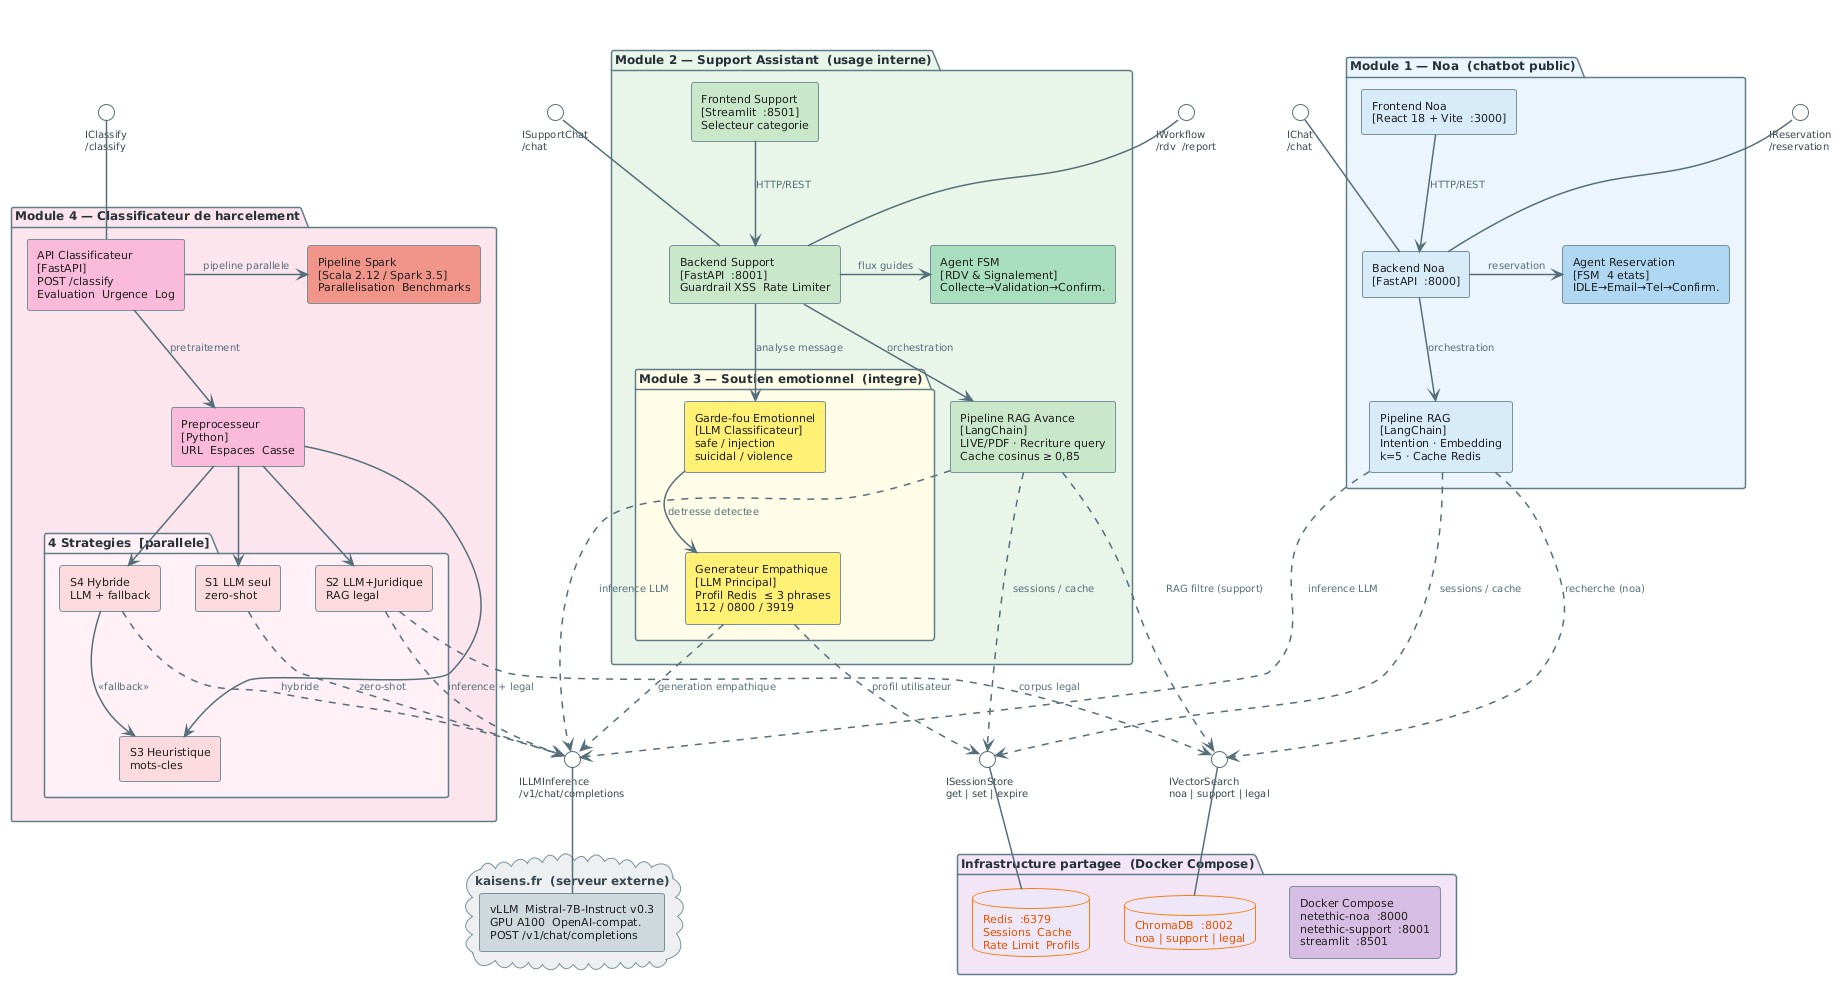
\includegraphics[width=1.2\textwidth]{diagramme/12_composants_architecture.png}
\caption{Diagramme de composants — Architecture globale du système}
\label{fig:composants_global}
\end{figure}

\subsection{Composants partagés}

Les composants suivants sont utilisés par plusieurs modules :

\begin{itemize}
    \item \textbf{Serveur LLM partagé (kaisens.fr) :} Point central de génération de réponses
          en langage naturel pour les quatre modules.
          Il s'appuie sur vLLM avec le modèle Mistral-7B-Instruct v0.3 sur GPU NVIDIA A100,
          exposé via une interface compatible OpenAI (\texttt{POST /v1/chat/completions}).
    \item \textbf{Base documentaire vectorielle (ChromaDB) :} Stocke les extraits de documents
          indexés pour la recherche par similarité sémantique.
          Chaque module possède sa propre collection : l'assistant Noa et l'assistant technique
          embarquent ChromaDB directement dans leur conteneur API,
          tandis que le Classificateur l'instancie comme service Docker dédié.
    \item \textbf{Gestionnaire de mémoire (Redis) :} Assure la persistance des sessions
          conversationnelles, le cache sémantique cosinus et la limitation de débit \cite{redis}.
    \item \textbf{Orchestrateur LangChain :} Coordonne les étapes de traitement
          pour les modules conversationnels (Noa, Support, Soutien émotionnel) :
          classification d'intention, recherche documentaire, appel LLM
          et gestion de session \cite{langchain}.
    \item \textbf{Conteneurisation Docker :} Chaque module est déployé dans sa propre stack
          Docker Compose isolée, garantissant la reproductibilité, la portabilité
          et l'indépendance entre modules \cite{docker}.
\end{itemize}

\subsection{Architecture de déploiement}

Chaque module est déployé de manière indépendante dans sa propre stack Docker Compose.
Cette isolation garantit qu'un module peut être mis à jour, redémarré ou remplacé
sans affecter les autres.
La Figure~\ref{fig:deploiement} présente la vue d'ensemble du déploiement avec les quatre stacks et le LLM partagé.
Les diagrammes de déploiement détaillés de chaque module sont fournis dans les sections correspondantes.

\begin{figure}[H]
\centering
\hspace*{-0.1\textwidth}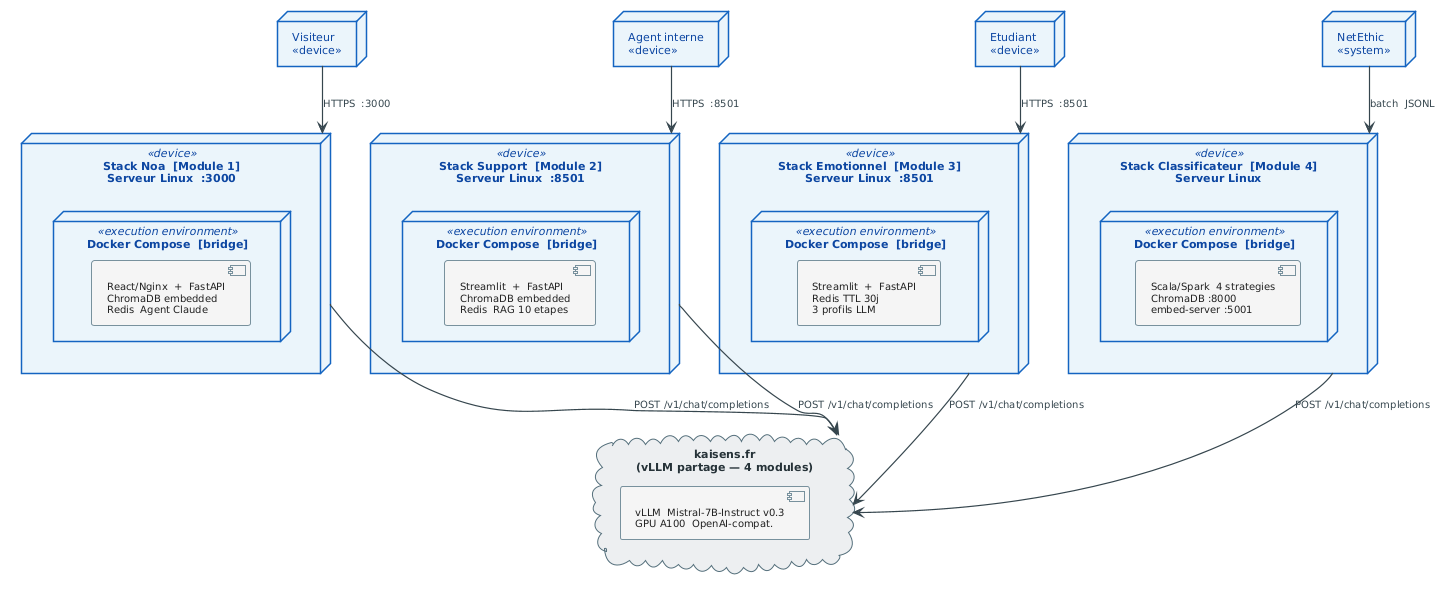
\includegraphics[width=1.2\textwidth]{diagramme/13_deploiement_uml.png}
\caption{Vue d'ensemble du déploiement — 4 stacks indépendantes de la plateforme NetEthic AI}
\label{fig:deploiement}
\end{figure}

% ─────────────────────────────────────────────────────────────────────────────
\section{Module 1 — Assistant Noa}

\subsection{Conception générale}

Noa est l'assistant virtuel accessible sur le site public de Netethic.
Son architecture repose sur un pipeline à cinq étapes :
classification de l'intention, vérification du cache, recherche documentaire,
génération de la réponse et mise à jour du cache.

\textbf{Routage par intention.}
Chaque message est classifié avant tout traitement.
Les salutations et demandes hors sujet reçoivent des réponses prédéfinies immédiates,
court-circuitant le pipeline RAG complet.

\textbf{Stratégie parent-enfant.}
Les documents sont indexés à deux niveaux : les segments courts (enfants) servent
à la recherche par similarité sémantique, tandis que les segments longs (parents)
sont transmis au LLM pour générer une réponse contextuellement riche.

\textbf{Normalisation des questions fréquentes.}
Deux questions au sens identique partagent la même réponse mémorisée,
grâce à une normalisation par synonymes avant la consultation du cache Redis.

\textbf{Agent de réservation.}
Un automate à états finis guide l'utilisateur lors de la collecte de son adresse
e-mail et de son numéro de téléphone pour planifier une démonstration.

\subsection{Diagramme de composants}

La Figure~\ref{fig:composants_noa} illustre l'organisation interne du module Noa en trois couches (présentation, métier et données) ainsi que les interactions entre ses composants principaux.

\begin{figure}[H]
\centering
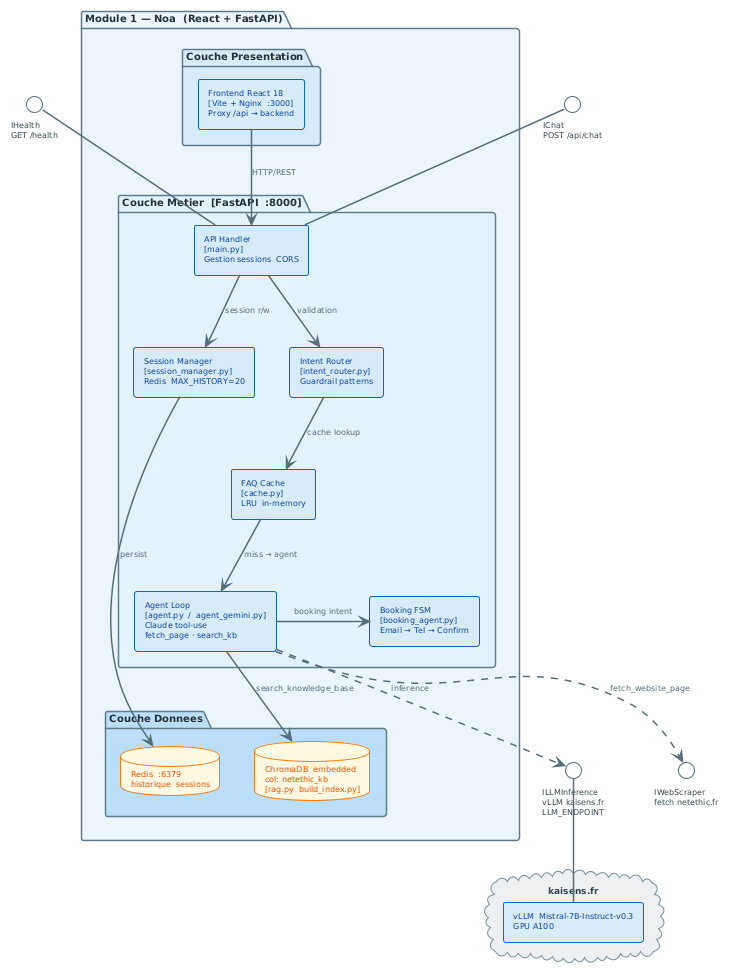
\includegraphics[width=\textwidth]{diagramme/18_composants_noa.png}
\caption{Diagramme de composants — Assistant Noa}
\label{fig:composants_noa}
\end{figure}

\subsection{Diagramme de déploiement}

La Figure~\ref{fig:deploiement_noa} présente la stack Docker Compose du module Noa avec ses conteneurs et leurs interconnexions.

\begin{figure}[H]
\centering
\hspace*{-0.1\textwidth}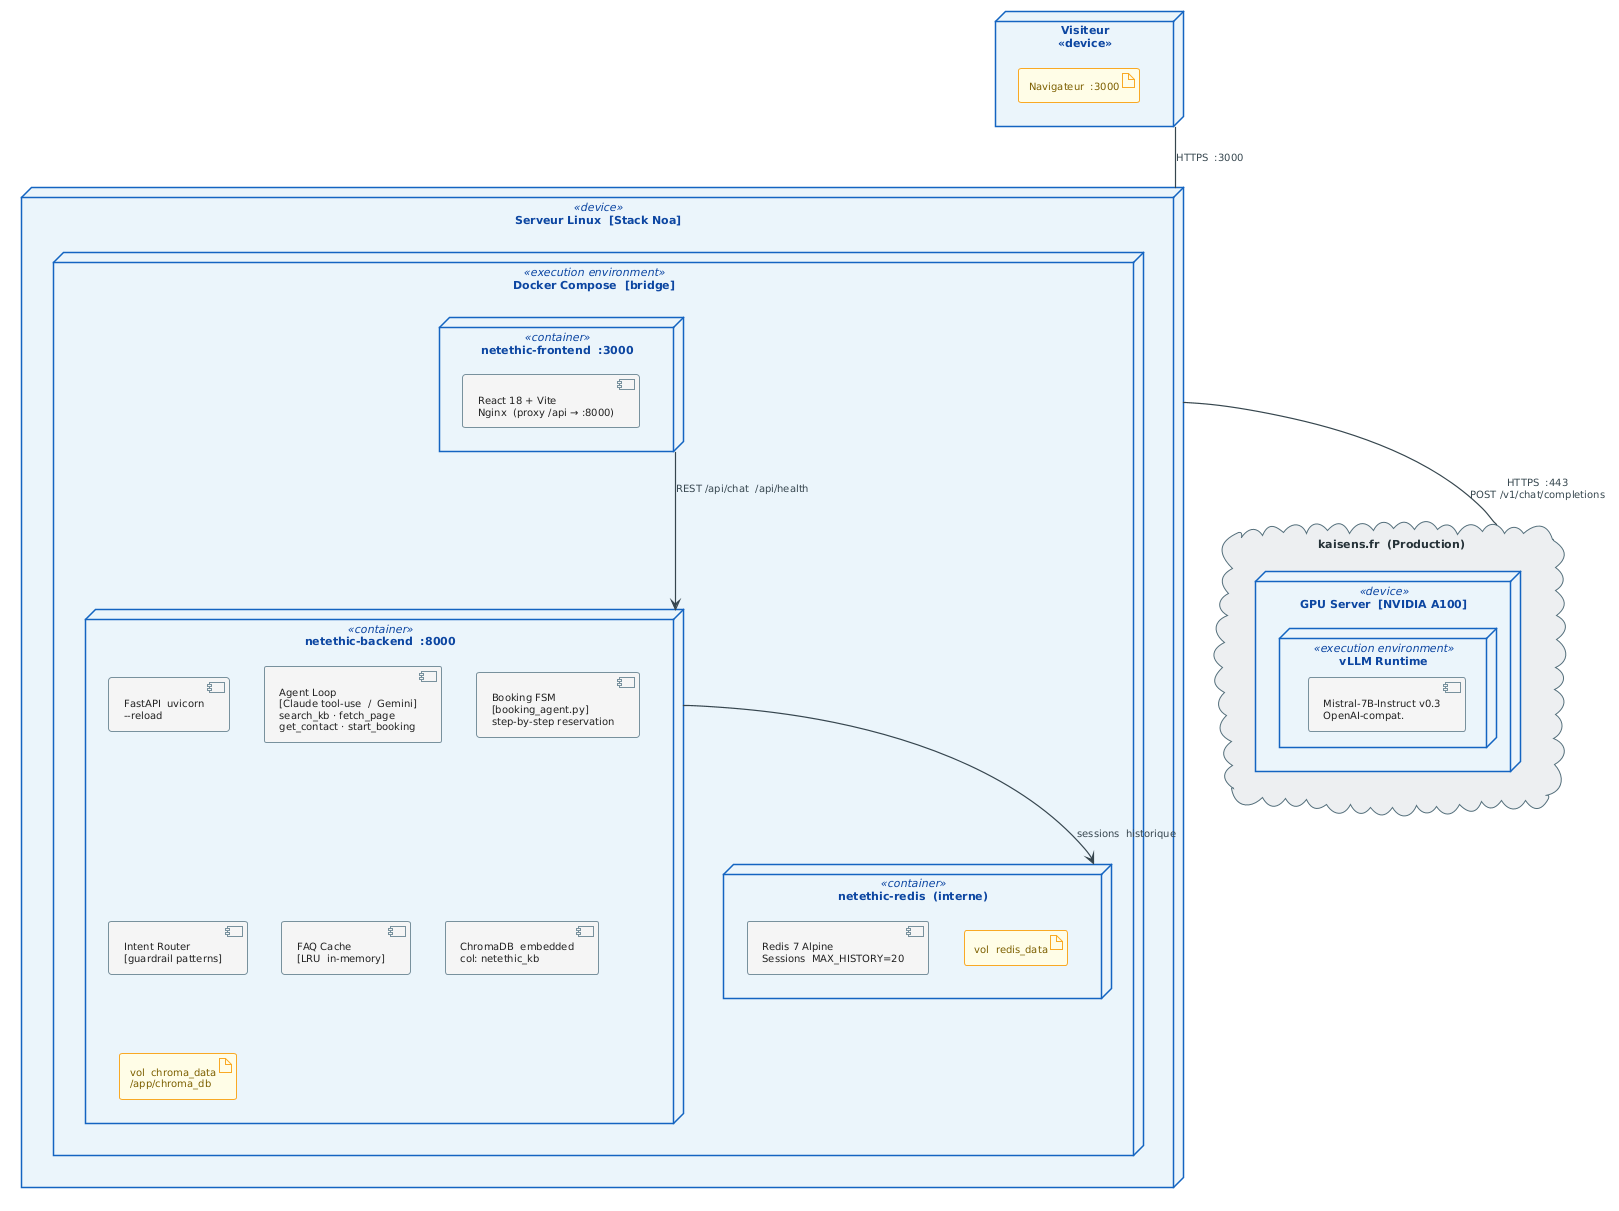
\includegraphics[width=1.2\textwidth]{diagramme/14_deploiement_noa.png}
\caption{Diagramme de déploiement — Assistant Noa (stack Docker Compose)}
\label{fig:deploiement_noa}
\end{figure}

\subsection{Diagramme de séquences}

La Figure~\ref{fig:seq_noa} illustre le déroulement d'une interaction typique avec Noa
pour une question factuelle.

\begin{figure}[H]
\centering
\hspace*{-0.1\textwidth}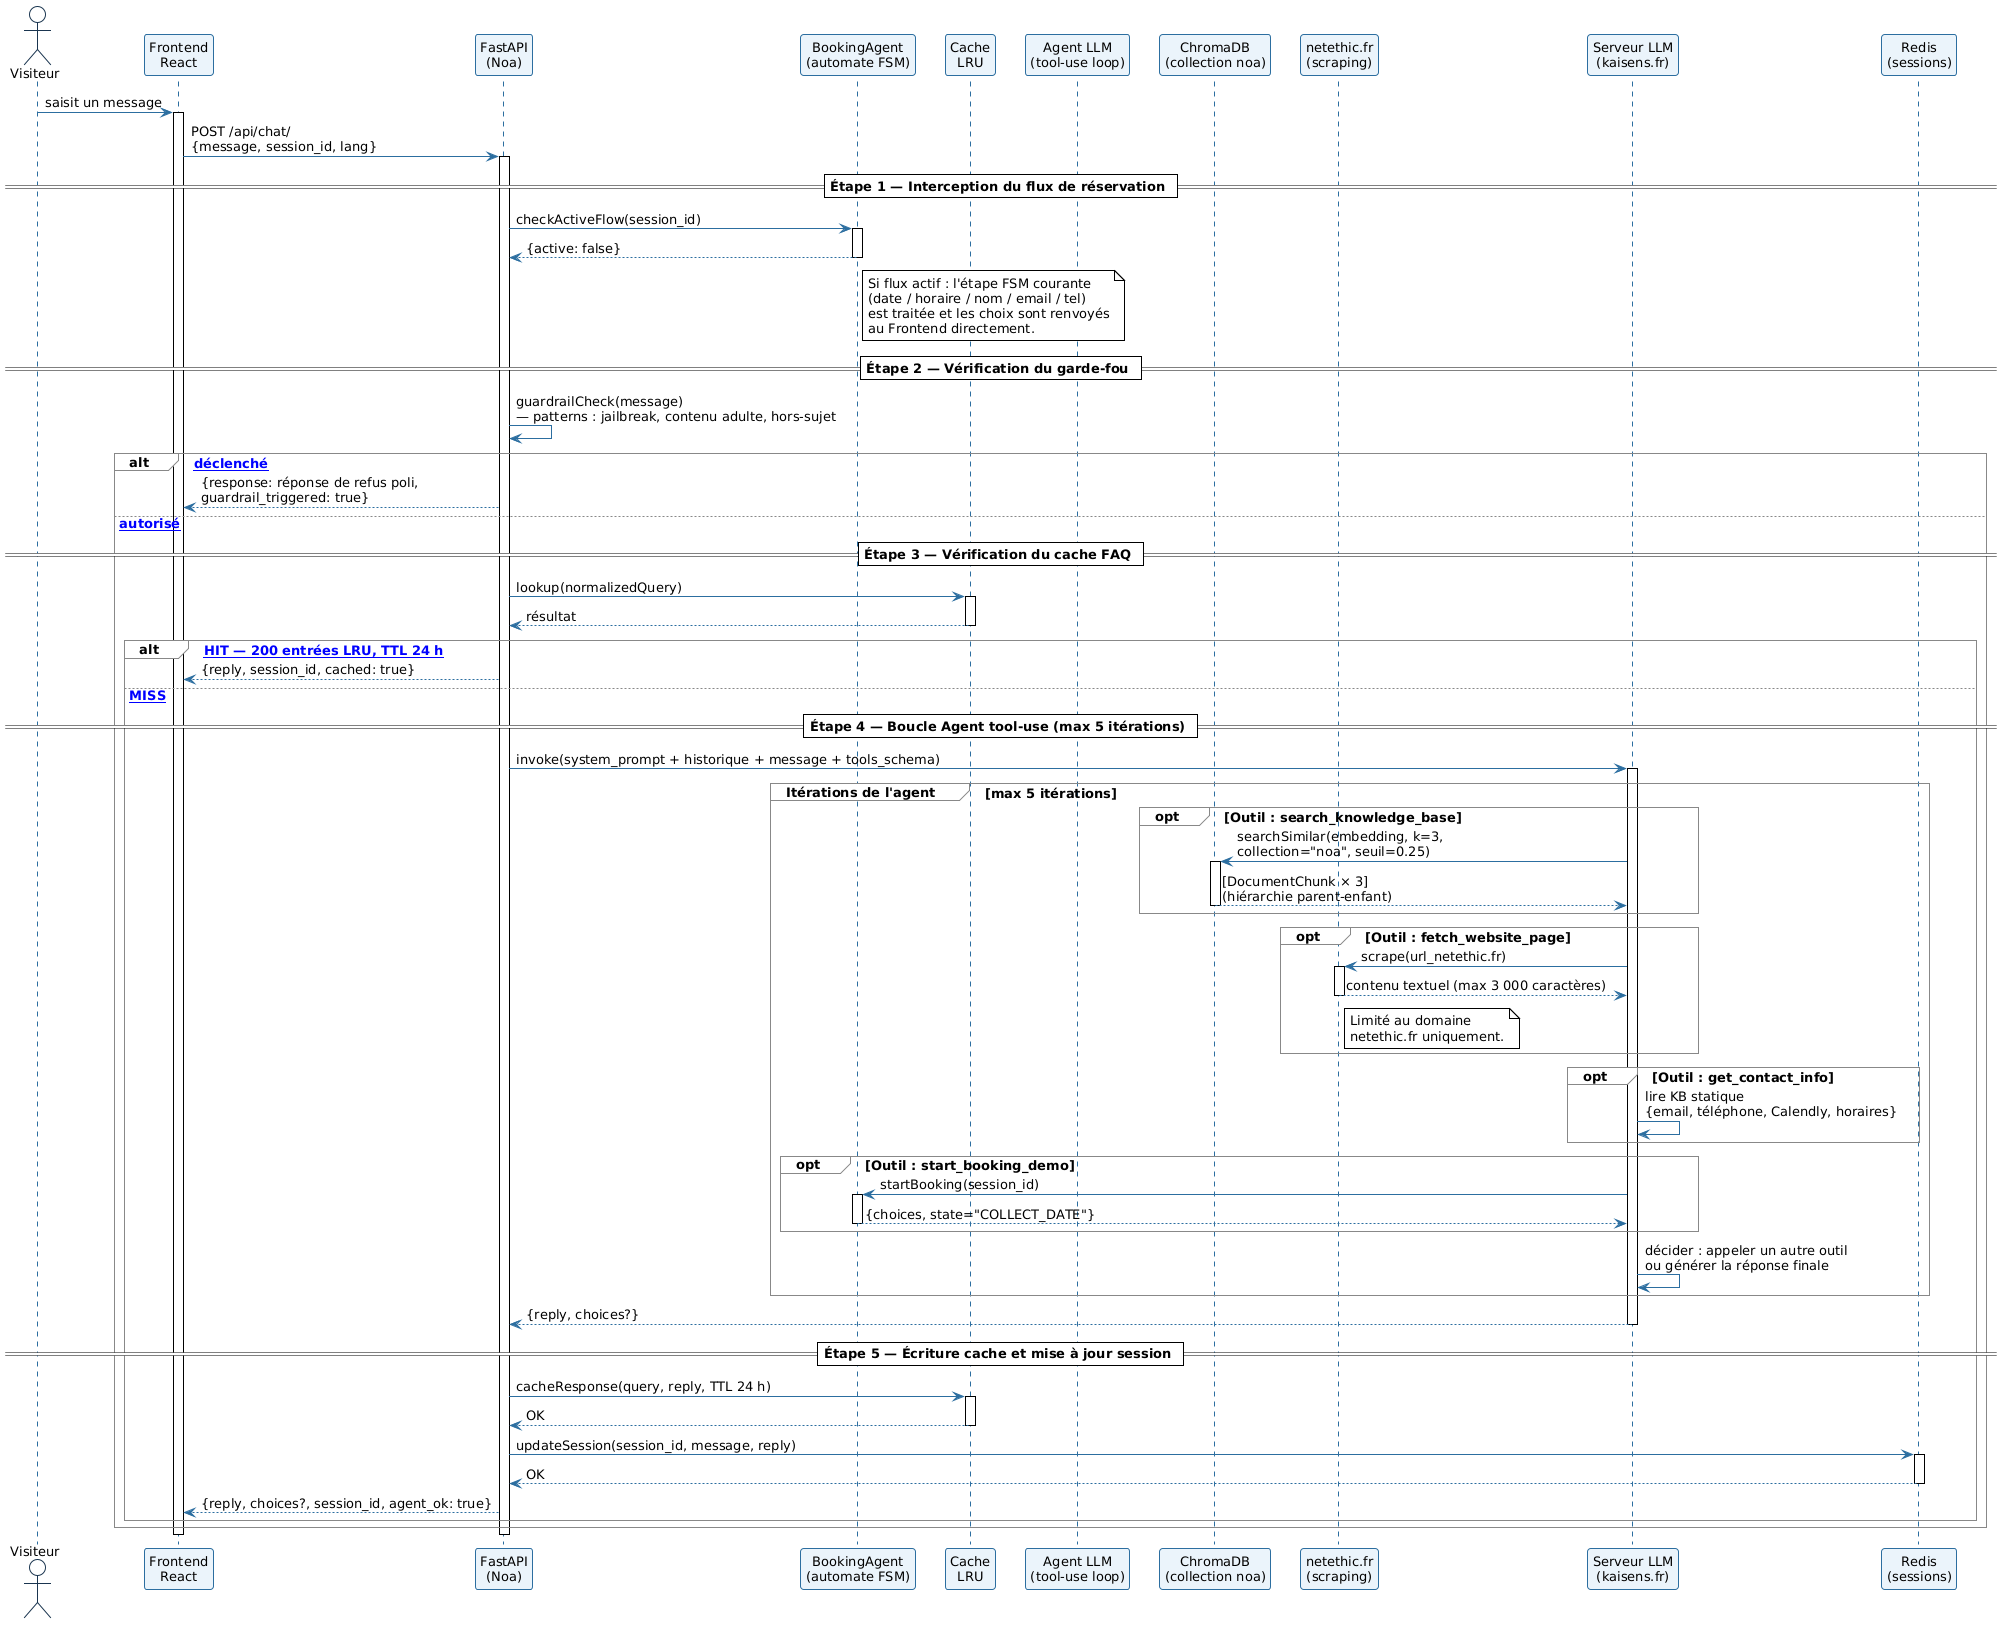
\includegraphics[width=1.2\textwidth]{diagramme/04_sequence_noa.png}
\caption{Diagramme de séquences — Assistant Noa (question factuelle)}
\label{fig:seq_noa}
\end{figure}


% ─────────────────────────────────────────────────────────────────────────────
\section{Module 2 — Assistant technique}

\subsection{Conception générale}

L'\textit{assistant technique} est l'assistant de support technique
destiné aux utilisateurs internes de la plateforme.
Son pipeline repose sur les mêmes composants partagés que l'assistant Noa
(serveur LLM, ChromaDB, Redis, LangChain),
mais introduit deux mécanismes architecturaux distincts.

\textbf{Double pipeline LIVE/PDF.}
À l'ouverture de session, la plateforme injecte un instantané JSON du tableau de bord
directement dans la session utilisateur.
Un classificateur d'intention LLM sépare ensuite les questions portant sur des métriques
en temps réel (\textit{LIVE}) des questions documentaires (\textit{PDF}).
Les premières sont traitées à partir des données de session uniquement,
sans appel à ChromaDB ; les secondes suivent le pipeline RAG standard.

\textbf{Flux de repli guidés.}
Lorsqu'aucun document pertinent n'est trouvé, le frontend déclenche trois flux
conversationnels à états finis : prise de rendez-vous, signalement de dysfonctionnement
(avec description auto-générée à partir de l'historique) et accès au portail de support.
Les informations d'identité de l'utilisateur, déjà présentes en session, pré-remplissent
les formulaires sans ressaisie.

L'interface est développée en Streamlit pour un déploiement rapide côté interne.

\subsection{Diagramme de composants}

La Figure~\ref{fig:composants_support} illustre l'architecture interne de l'assistant technique et les interactions entre ses composants.

\begin{figure}[H]
\centering
\hspace*{-0.1\textwidth}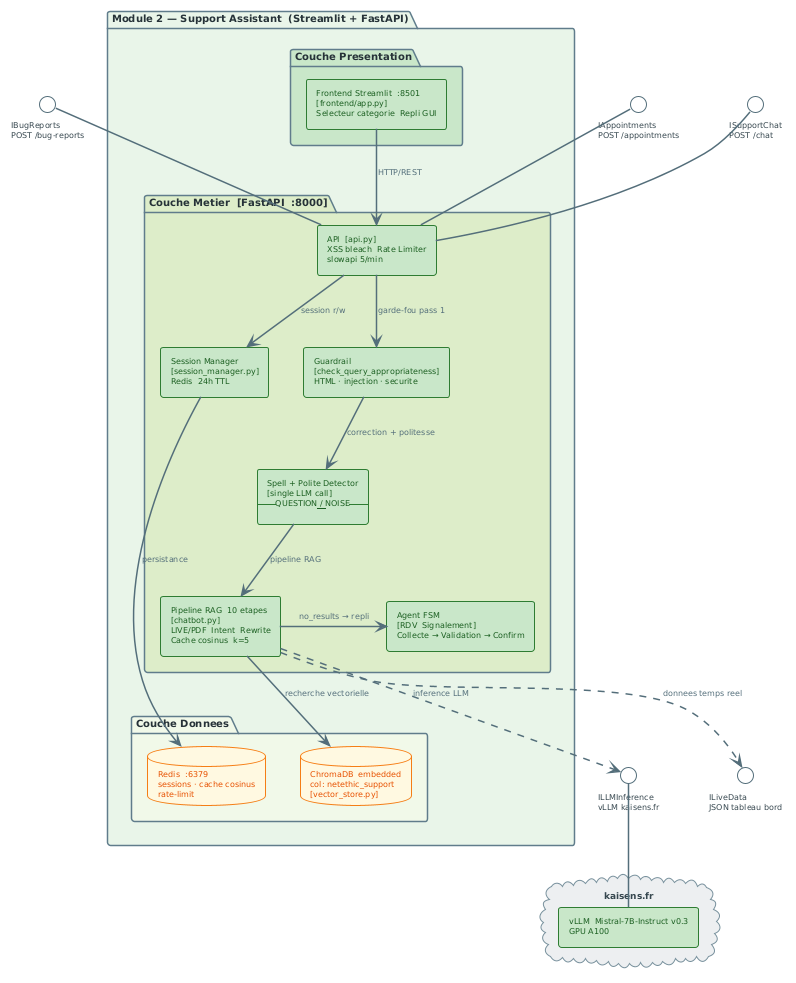
\includegraphics[width=1.2\textwidth]{diagramme/19_composants_support.png}
\caption{Diagramme de composants — Assistant technique}
\label{fig:composants_support}
\end{figure}

\subsection{Diagramme de déploiement}

La Figure~\ref{fig:deploiement_support} présente la stack Docker Compose de l'assistant technique avec ses conteneurs et leurs interconnexions.

\begin{figure}[H]
\centering
\hspace*{-0.1\textwidth}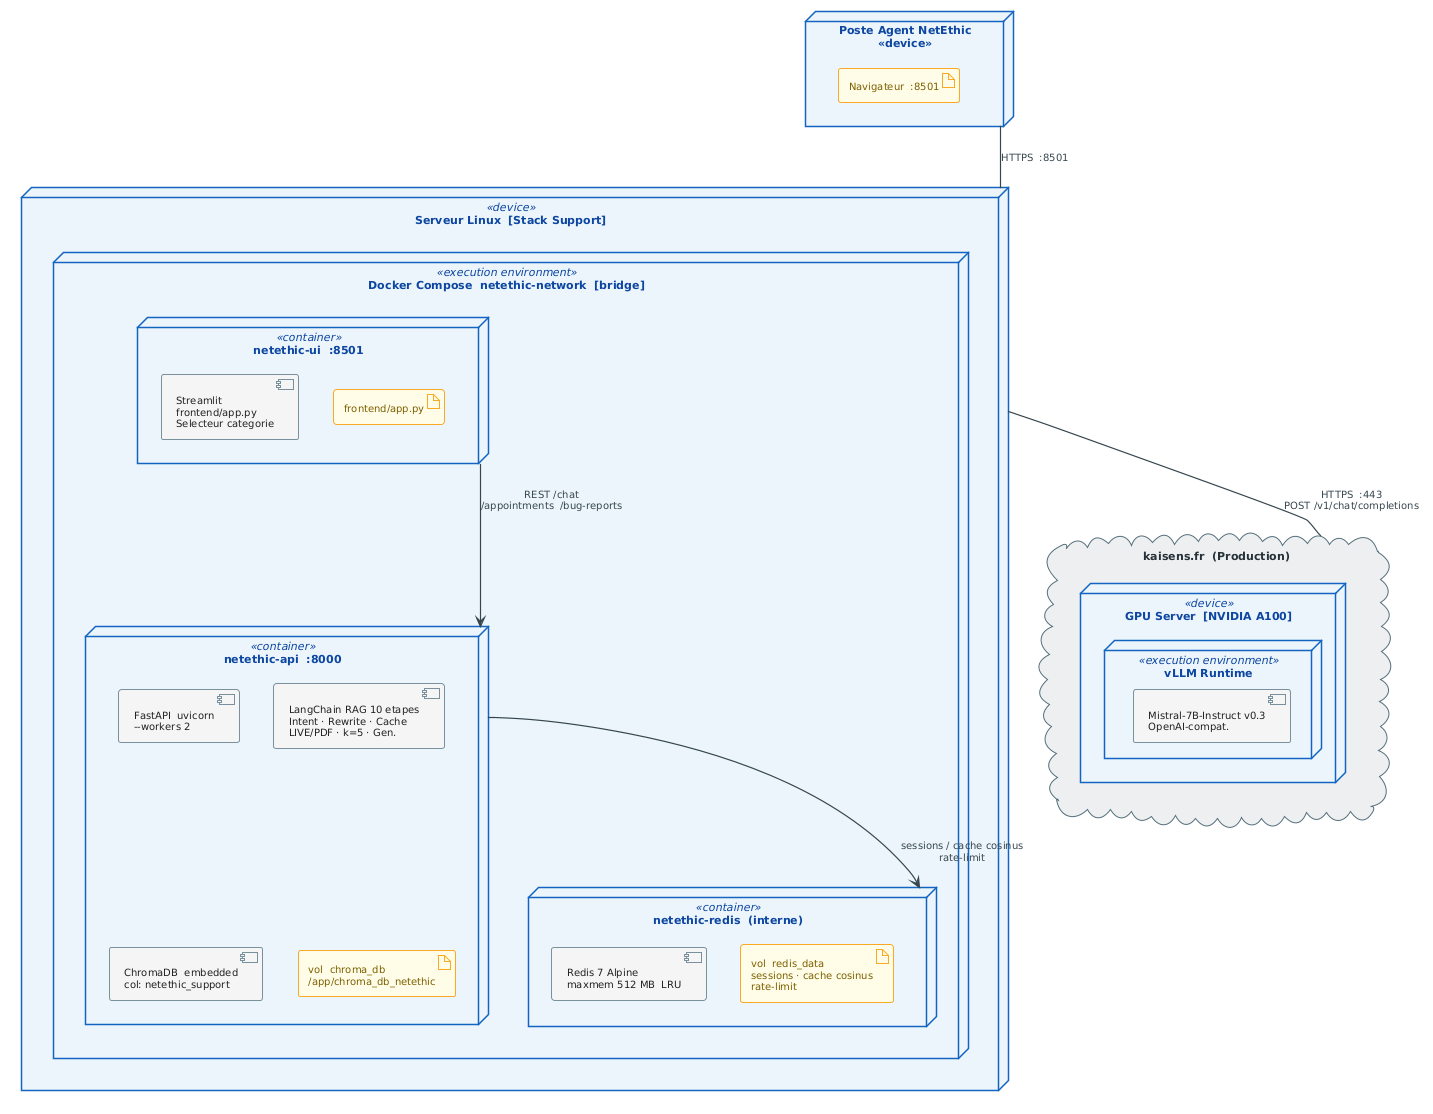
\includegraphics[width=1.2\textwidth]{diagramme/15_deploiement_support.png}
\caption{Diagramme de déploiement — Assistant technique (stack Docker Compose)}
\label{fig:deploiement_support}
\end{figure}

\subsection{Diagrammes de séquences}

Le traitement d'une question par l'assistant technique est décrit en trois parties.
La Figure~\ref{fig:seq_support_init} couvre la phase d'initialisation et de validation (étapes 1 à 10).

\begin{figure}[H]
\centering
\hspace*{-0.1\textwidth}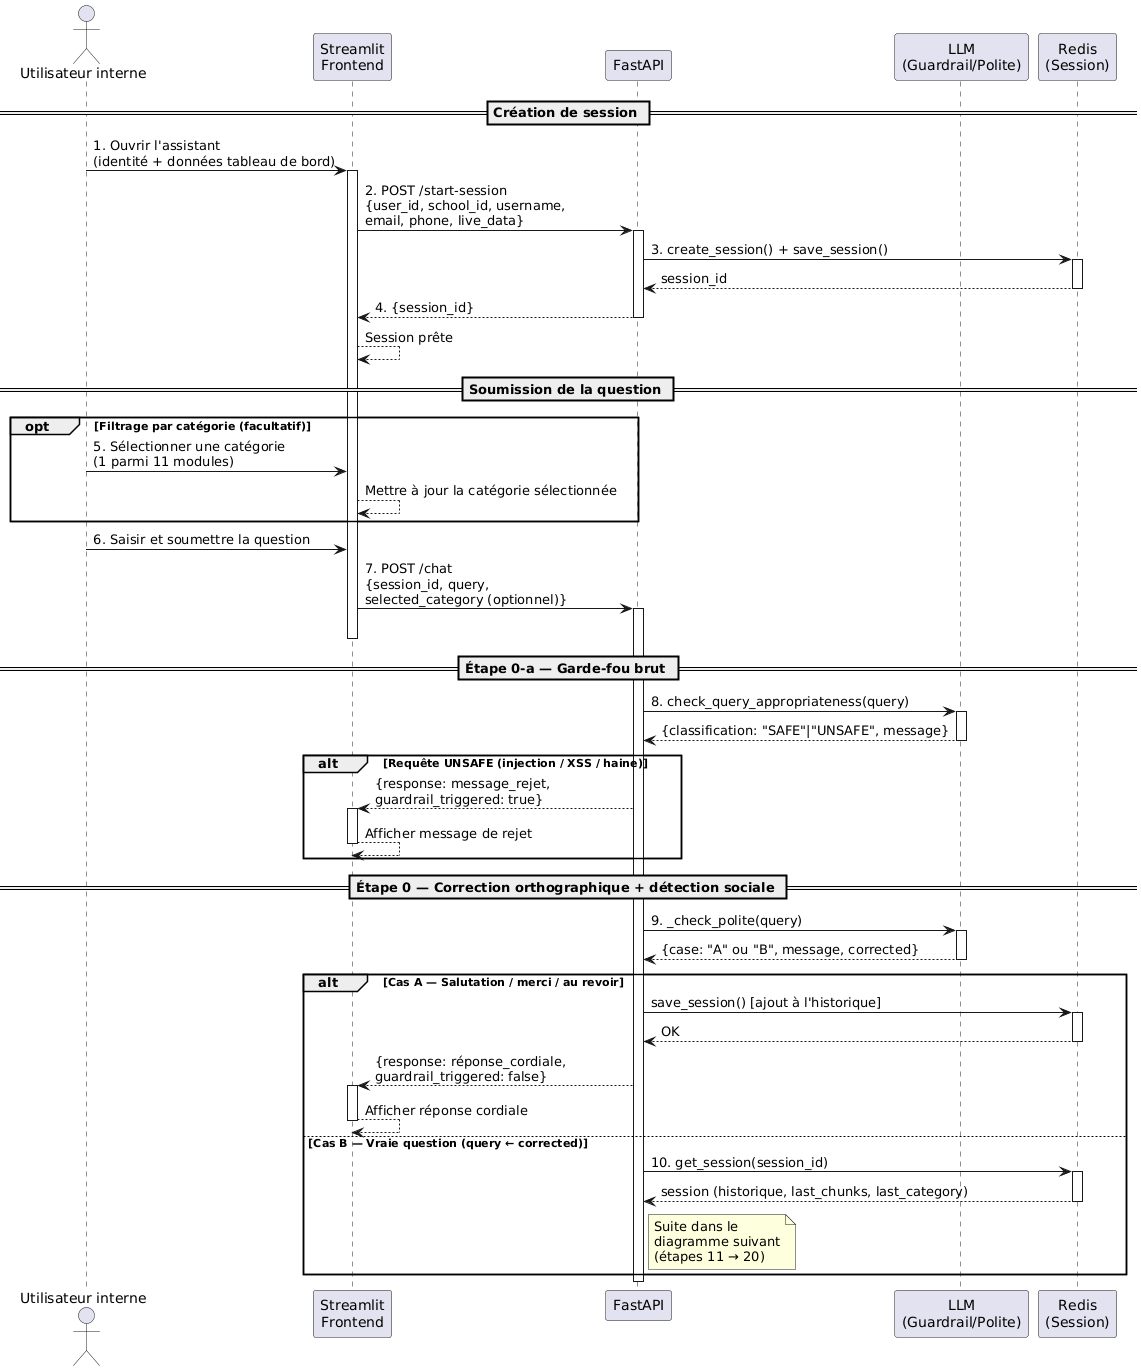
\includegraphics[width=1.15\textwidth]{diagramme/06a_sequence_support_init.png}
\caption{Diagramme de séquences — Assistant technique (1/3) : session et validation}
\label{fig:seq_support_init}
\end{figure}

La Figure~\ref{fig:seq_support} détaille le pipeline RAG (étapes 11 à 20).

\begin{figure}[H]
\centering
\hspace*{-0.1\textwidth}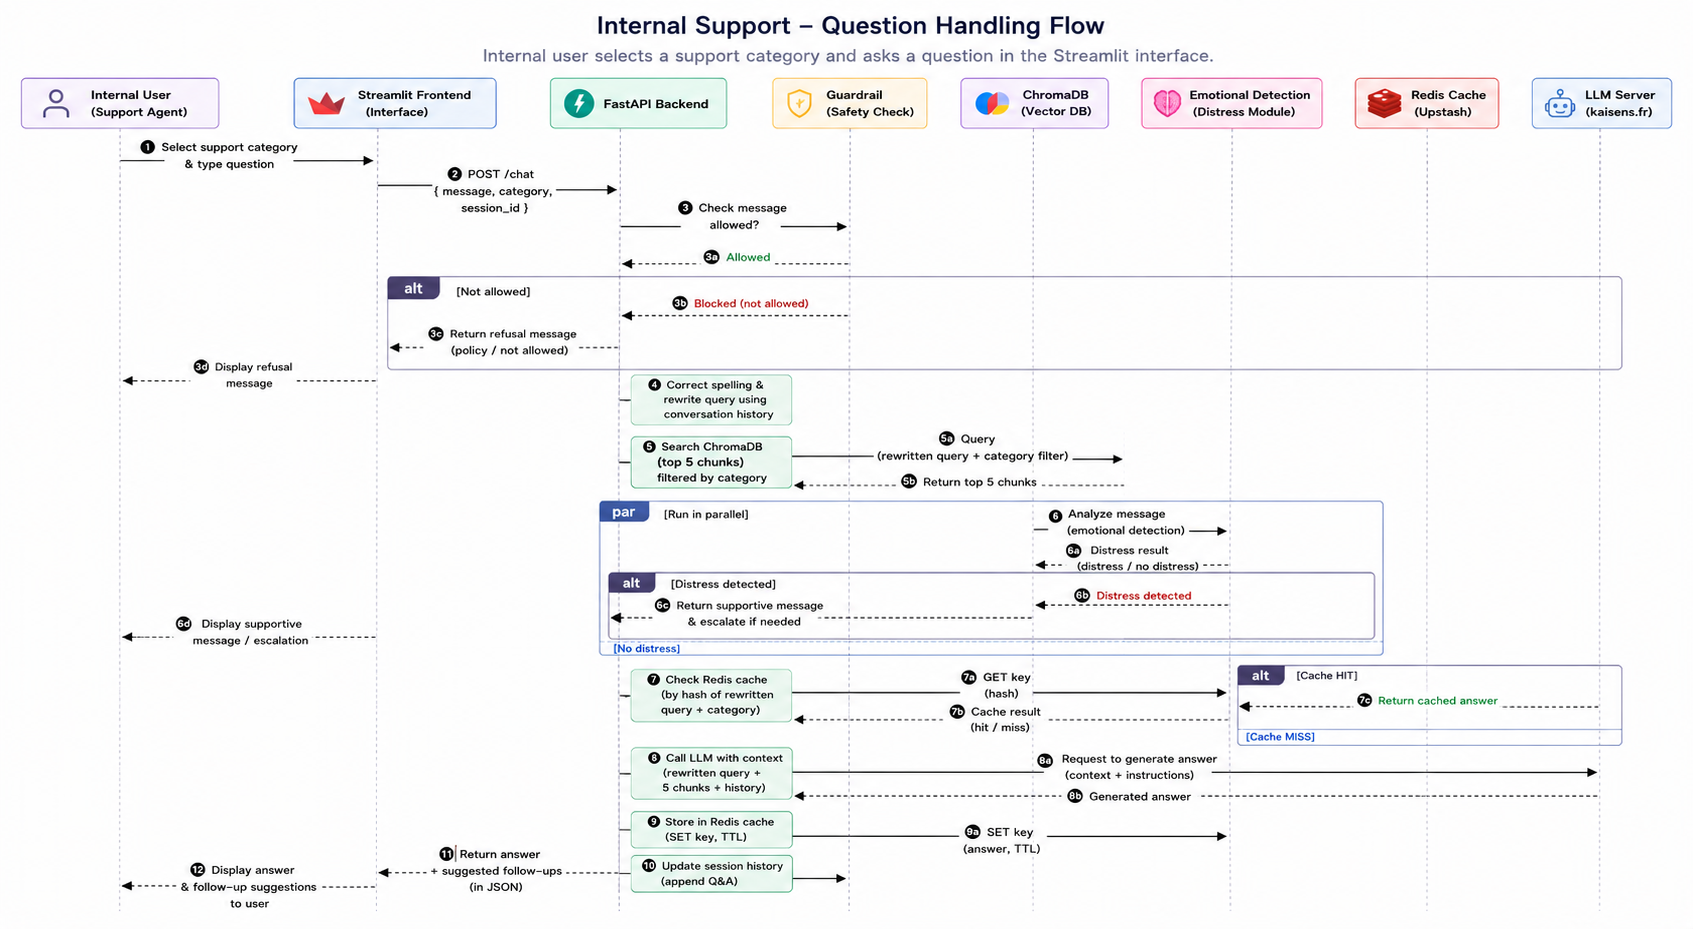
\includegraphics[width=1.15\textwidth]{diagramme/06_sequence_support.png}
\caption{Diagramme de séquences — Assistant technique (2/3) : pipeline RAG}
\label{fig:seq_support}
\end{figure}

La Figure~\ref{fig:seq_support_repli} illustre les flux de repli déclenchés
lorsqu'aucun document pertinent n'est trouvé dans ChromaDB (\texttt{no\_results=true}).
L'utilisateur dispose alors de deux options : prendre un rendez-vous ou signaler un bug.
Dans les deux cas, LangChain génère automatiquement une description à partir
de l'historique de conversation avant de soumettre la requête à l'API NetEthic.

\begin{figure}[H]
\centering
\hspace*{-0.1\textwidth}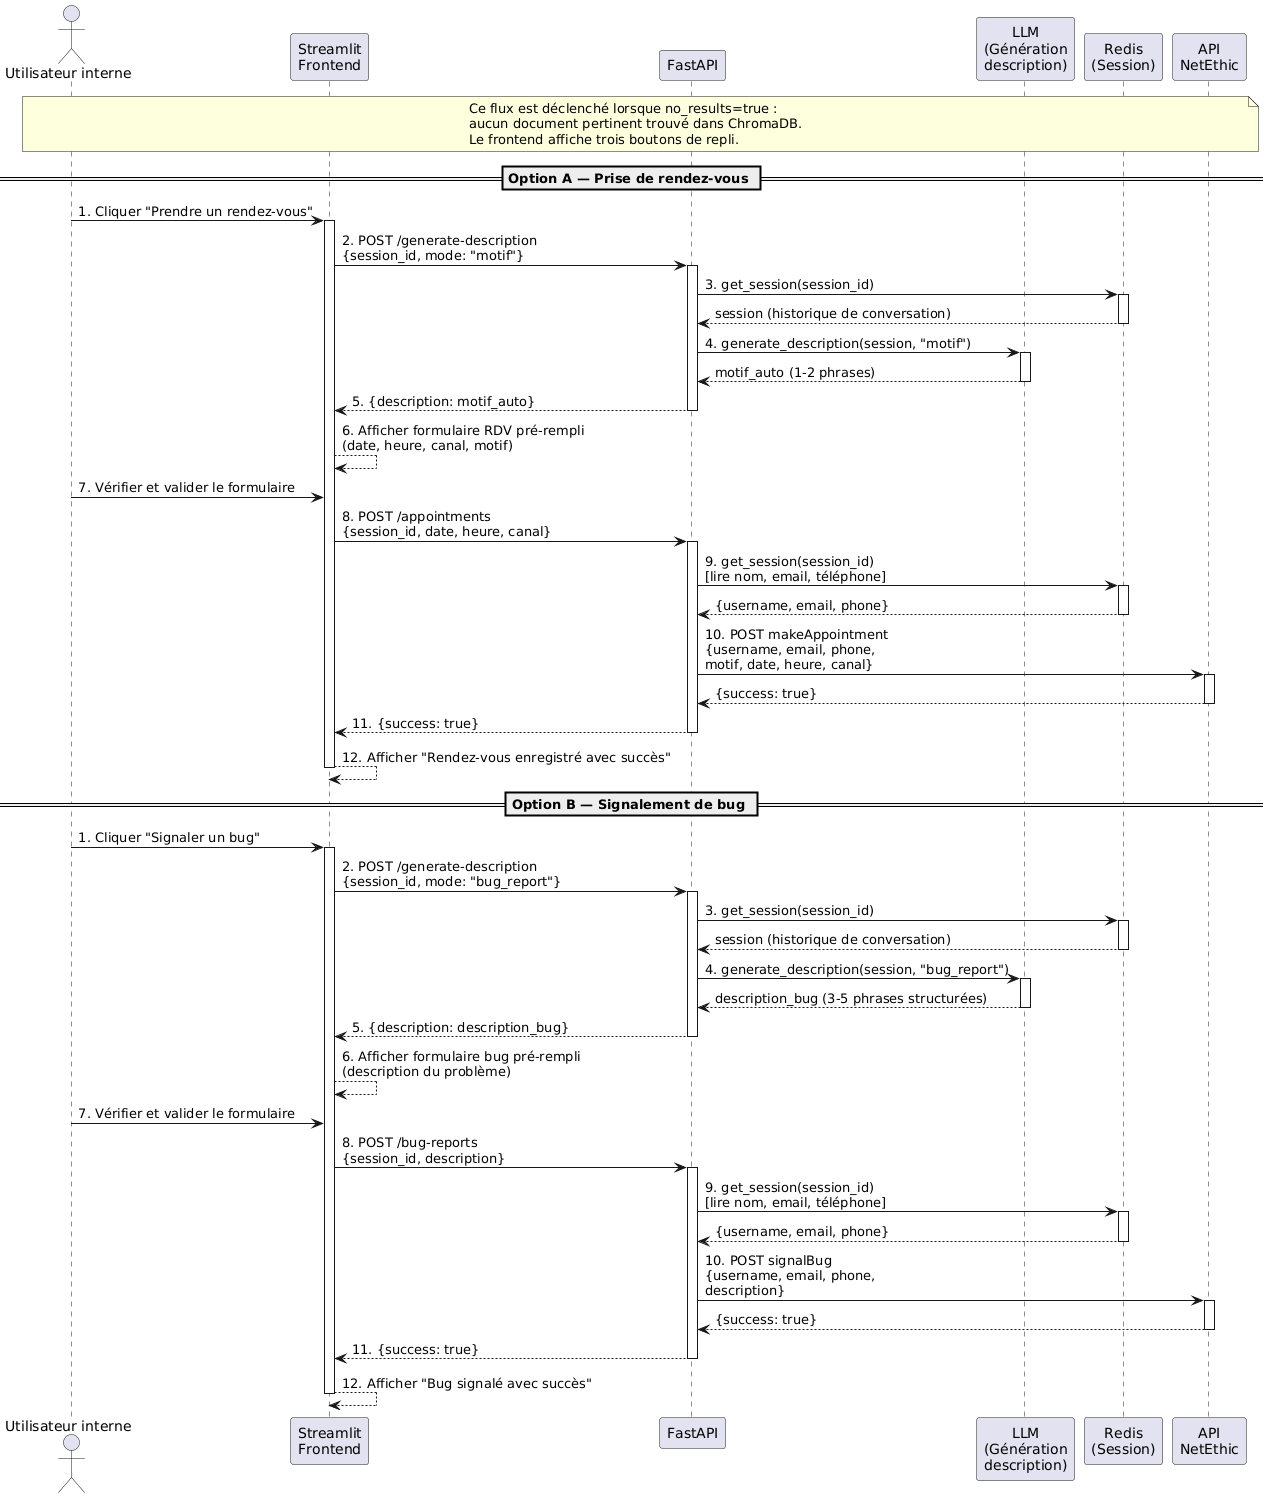
\includegraphics[width=1.15\textwidth]{diagramme/06b_sequence_support_repli.png}
\caption{Diagramme de séquences — Assistant technique (3/3) : flux de repli}
\label{fig:seq_support_repli}
\end{figure}

\subsection{Diagramme d'activité}

La Figure~\ref{fig:activite_support} représente le flux de traitement complet
d'un message par l'assistant technique, depuis la validation initiale
jusqu'à la génération de la réponse, en incluant les chemins de repli.

\begin{figure}[H]
\centering
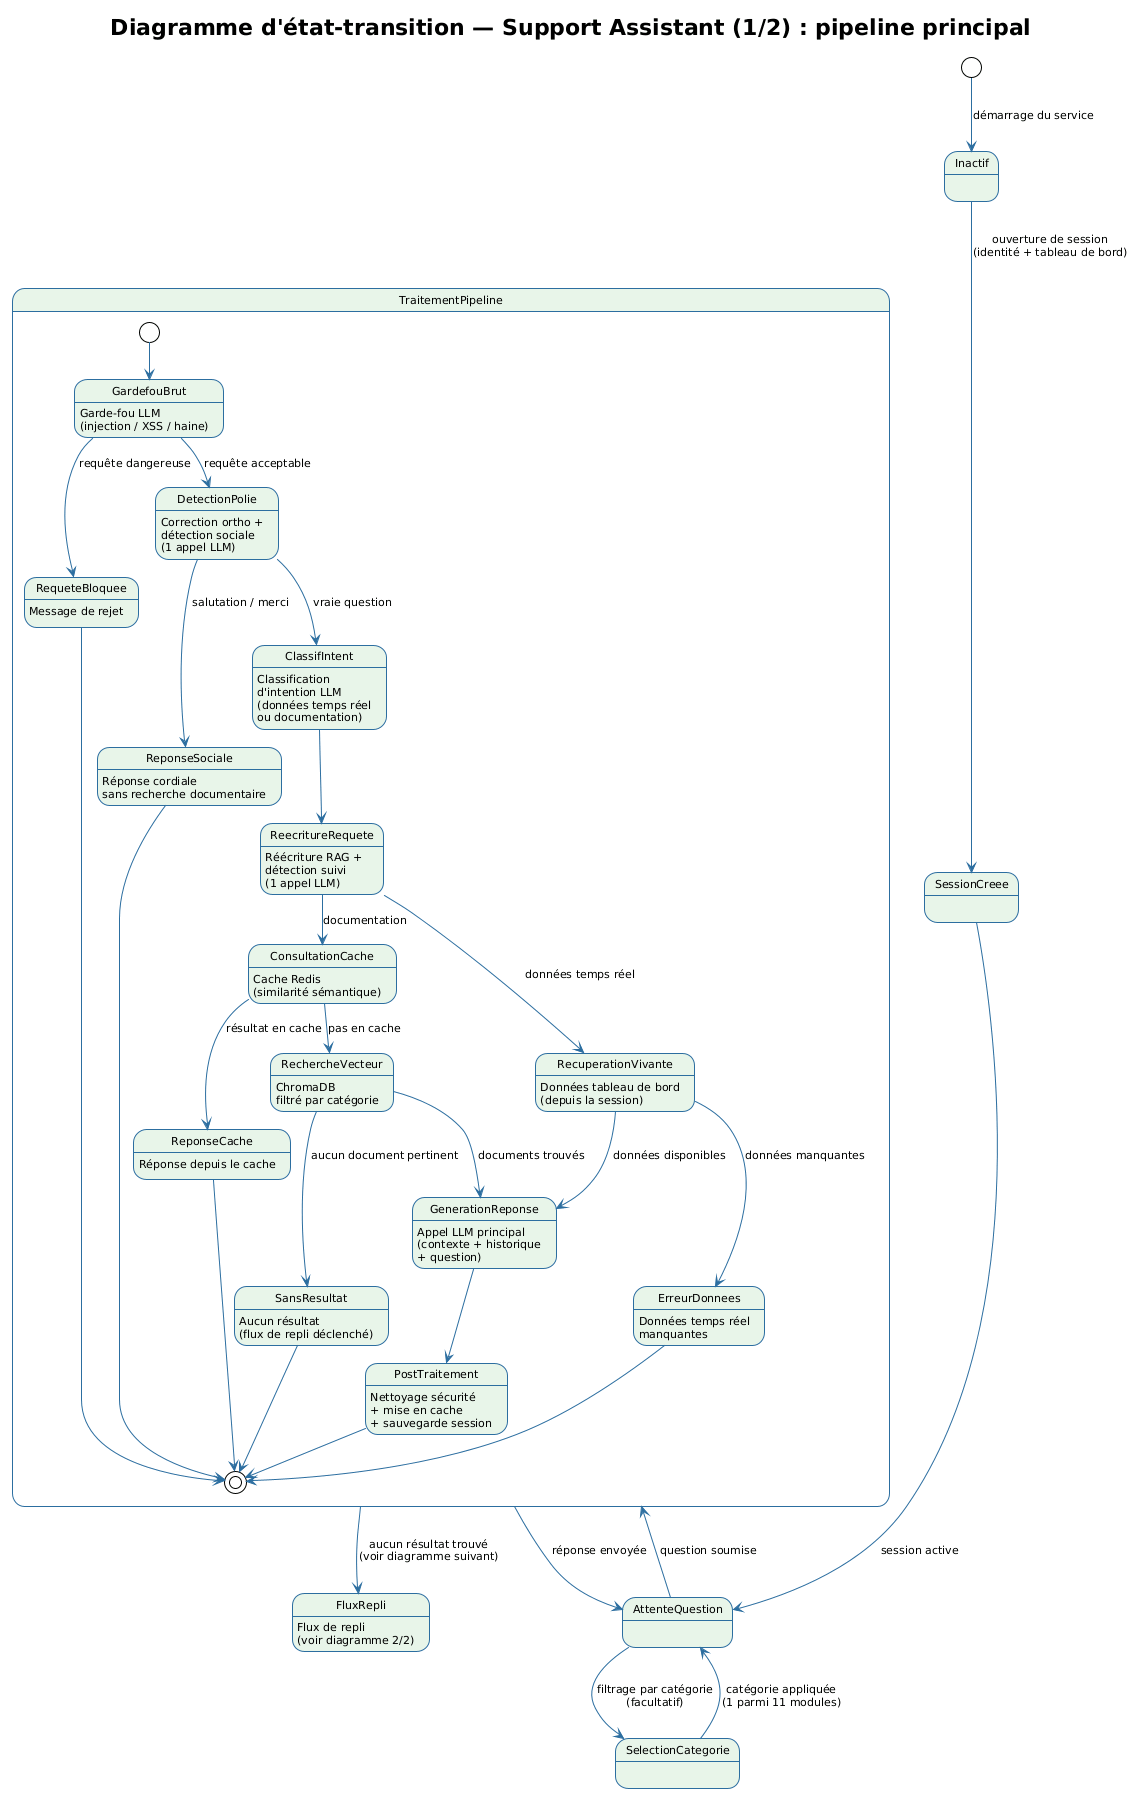
\includegraphics[width=0.95\textwidth]{diagramme/07a_etat_support_pipeline.png}
\caption{Diagramme d'activité — Assistant technique : pipeline et flux de repli}
\label{fig:activite_support}
\end{figure}

% ─────────────────────────────────────────────────────────────────────────────
\section{Module 3 — Assistant émotionnel}

\subsection{Conception générale}

L'assistant émotionnel est un assistant conversationnel dédié aux étudiants,
accessible via une interface Streamlit.
Il traite chaque message à travers un pipeline structuré reposant sur quatre mécanismes
complémentaires.

\textbf{Protection de l'échange.}
Chaque message passe par deux vérifications avant tout traitement :
une limitation du débit par fenêtre glissante Redis,
puis une analyse par un classifieur LLM à température nulle.
Les messages abusifs ou les tentatives de manipulation sont bloqués
à cette étape sans interrompre la session.

\textbf{Détection et réponse de crise.}
Si le classifieur identifie un signal de crise (idéation suicidaire ou intention de violence),
une réponse d'urgence est générée dans la langue de l'étudiant.
Les numéros d'aide sont ajoutés de façon systématique — jamais laissés à la discrétion du LLM.

\textbf{Mémoire persistante.}
Les informations partagées par l'étudiant (prénom, sources de stress, situation scolaire,
réussites) sont extraites automatiquement et stockées dans Redis avec une durée de vie
de trente jours. Ce profil enrichit le prompt système à chaque nouvelle session.

\textbf{Génération empathique.}
Pour les messages sûrs, l'assistant construit un prompt enrichi du profil mémorisé
et de l'historique de conversation, puis génère une réponse adaptée à la langue
et au contexte de l'étudiant, limitée à trois phrases.

\subsection{Diagramme de composants}

La Figure~\ref{fig:composants_emotionnel} illustre l'architecture en couches de l'assistant émotionnel et les interactions entre ses composants.

\begin{figure}[H]
\centering
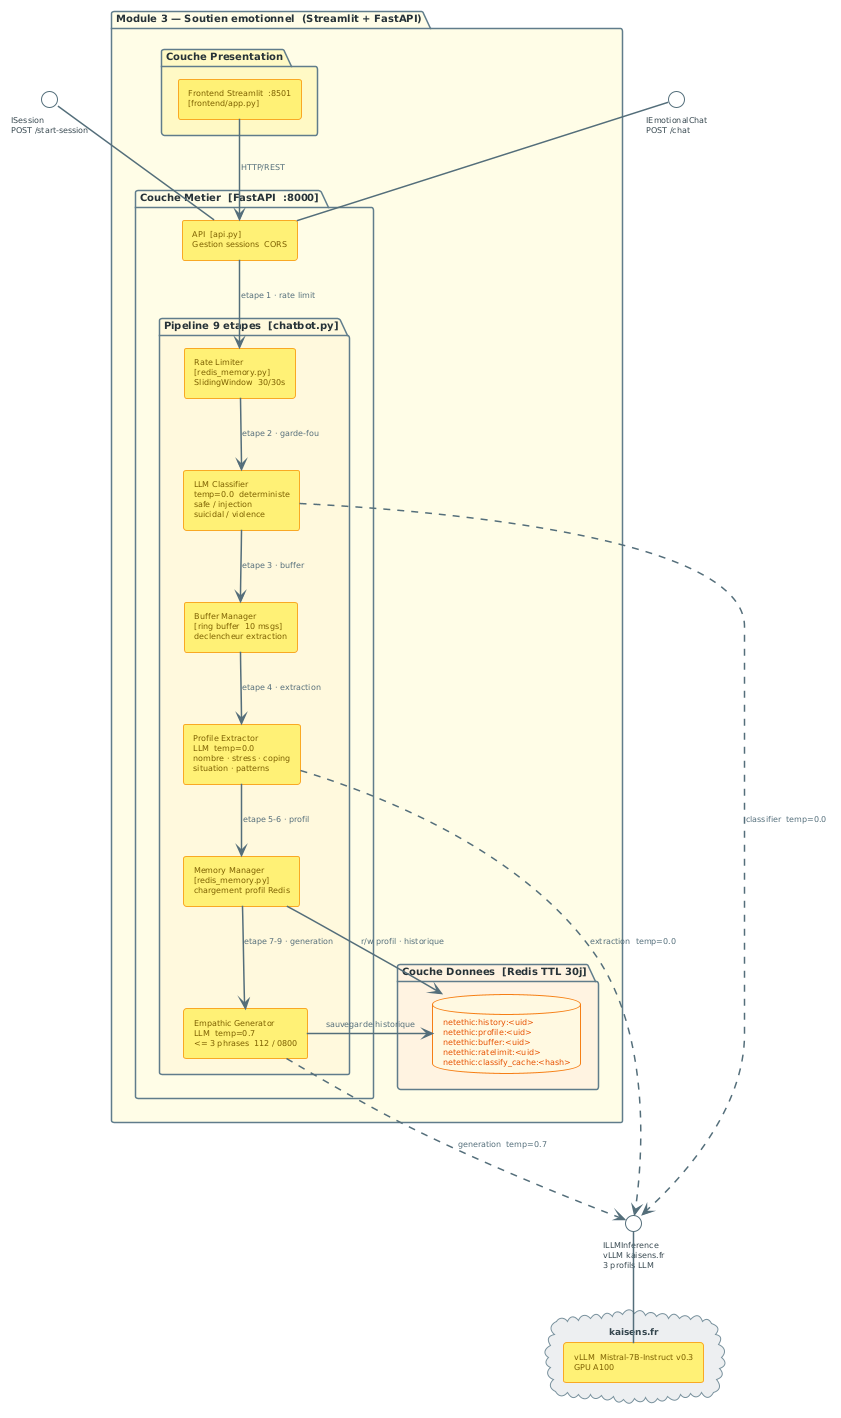
\includegraphics[width=\textwidth]{diagramme/20_composants_emotionnel.png}
\caption{Diagramme de composants — Assistant émotionnel}
\label{fig:composants_emotionnel}
\end{figure}

\subsection{Diagramme de déploiement}

La Figure~\ref{fig:deploiement_emotionnel} présente la stack Docker Compose de l'assistant émotionnel avec ses conteneurs et leurs interconnexions.

\begin{figure}[H]
\centering
\hspace*{-0.1\textwidth}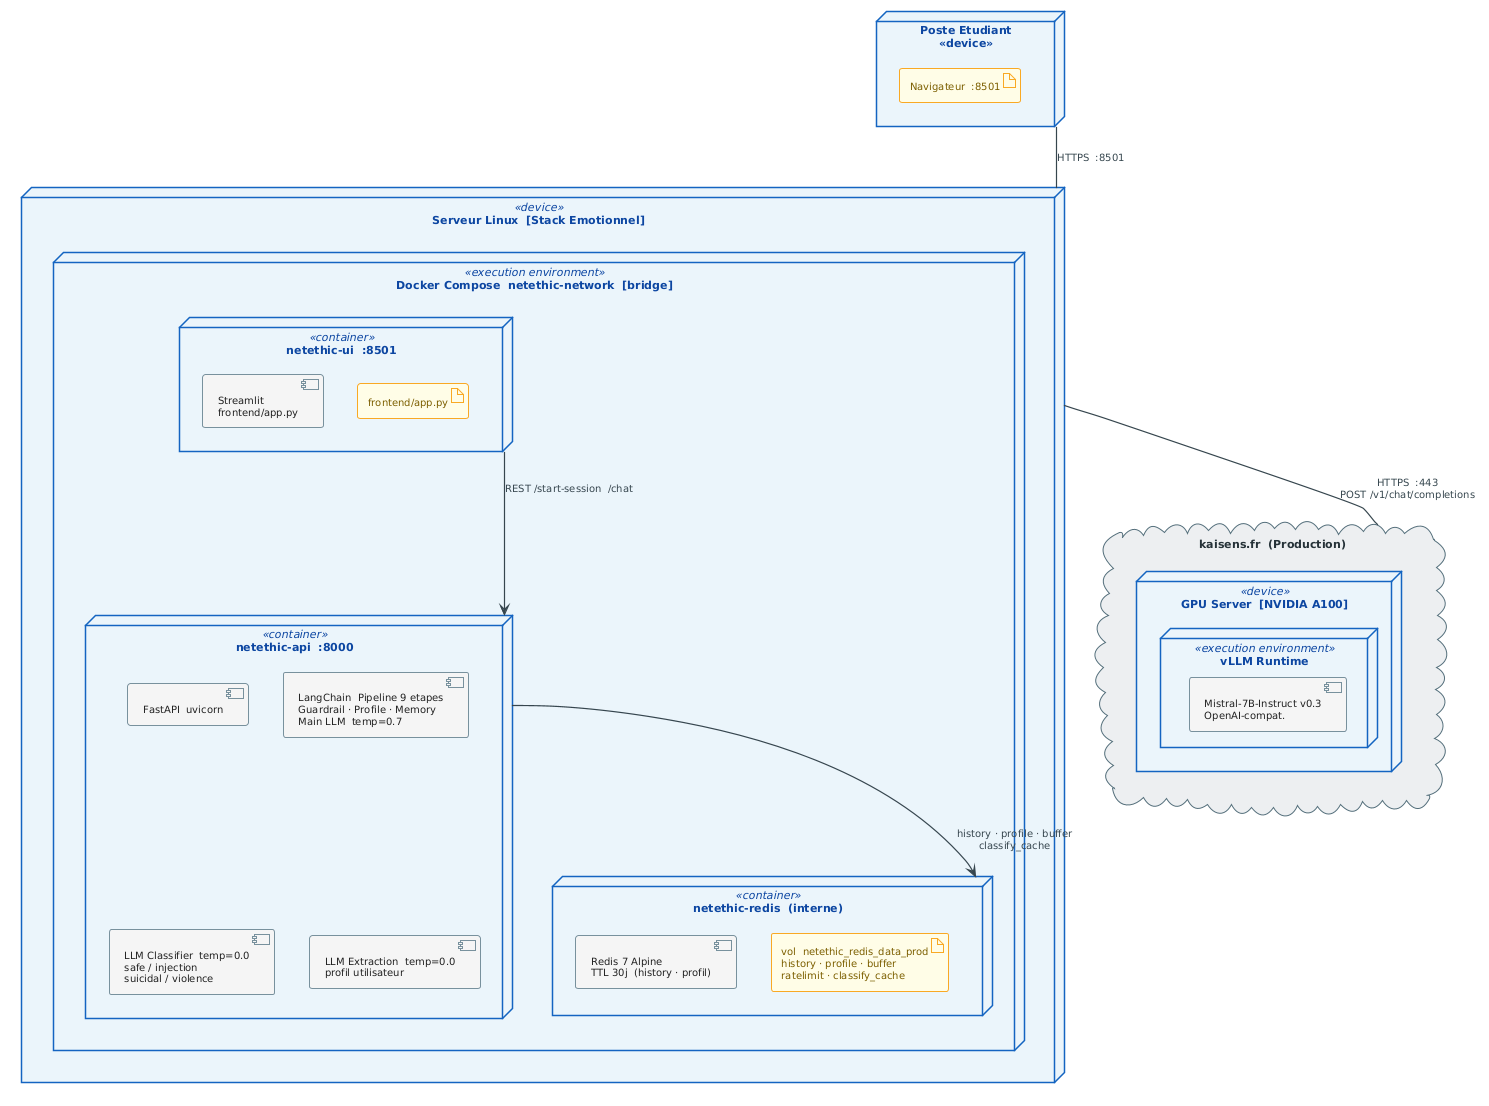
\includegraphics[width=1.2\textwidth]{diagramme/16_deploiement_emotionnel.png}
\caption{Diagramme de déploiement — Assistant émotionnel (stack Docker Compose)}
\label{fig:deploiement_emotionnel}
\end{figure}

\subsection{Diagramme de séquences}

La Figure~\ref{fig:seq_emotionnel_1} couvre les étapes 1 à 3 : validation de la session,
contrôle du débit et analyse par le garde-fou, avec ses quatre branches
(limite dépassée, contenu inapproprié, idéation suicidaire/violence, message sûr).

\begin{figure}[H]
\centering
\hspace*{-0.1\textwidth}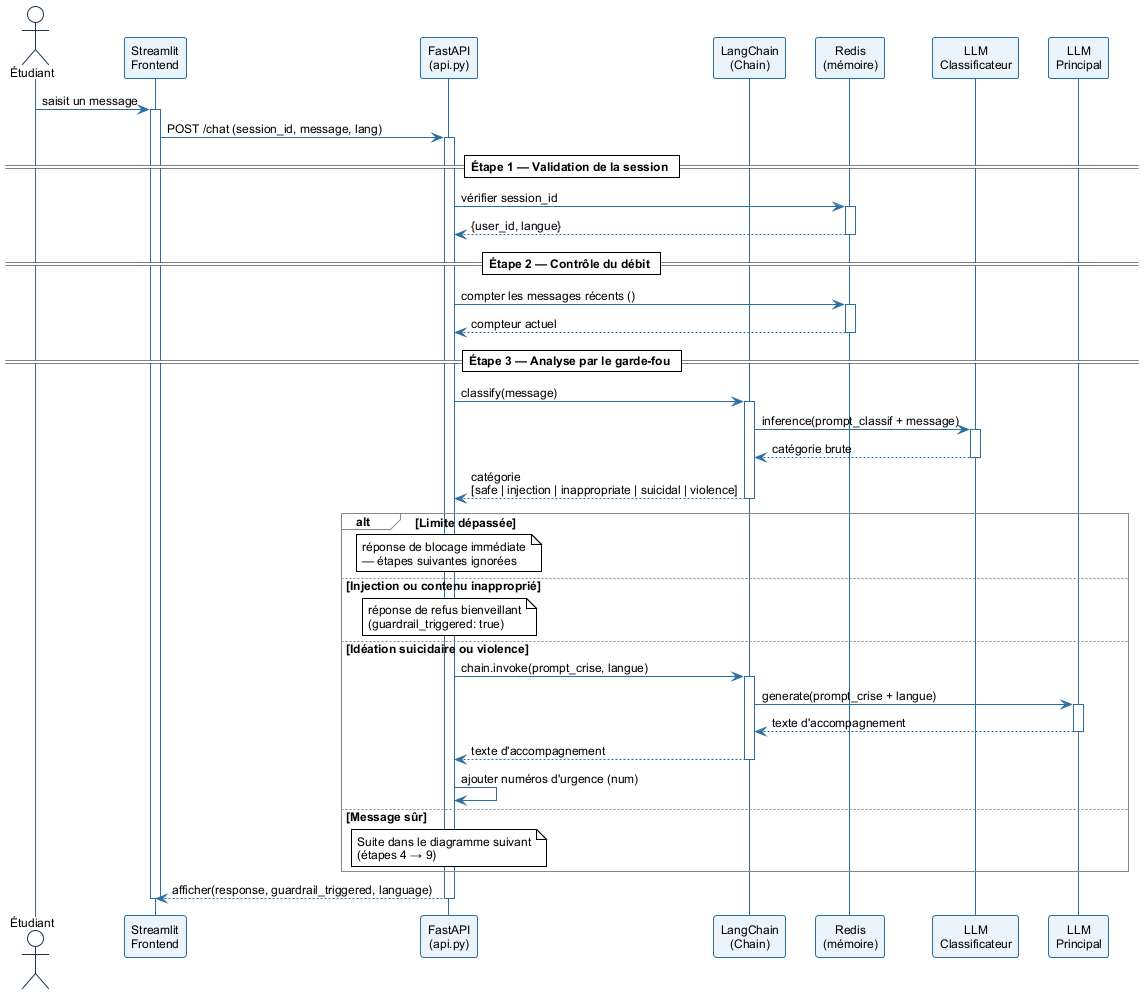
\includegraphics[width=1.15\textwidth]{diagramme/08b_sequence_emotionnel_1.png}
\caption{Diagramme de séquences — Assistant émotionnel (1/2) : validation et garde-fou}
\label{fig:seq_emotionnel_1}
\end{figure}

La Figure~\ref{fig:seq_emotionnel_2} détaille le chemin nominal (message sûr),
des étapes 4 à 9 : chargement du profil étudiant, enrichissement du prompt,
génération empathique par le LLM via LangChain, puis post-traitement et sauvegarde.

\begin{figure}[H]
\centering
\hspace*{-0.1\textwidth}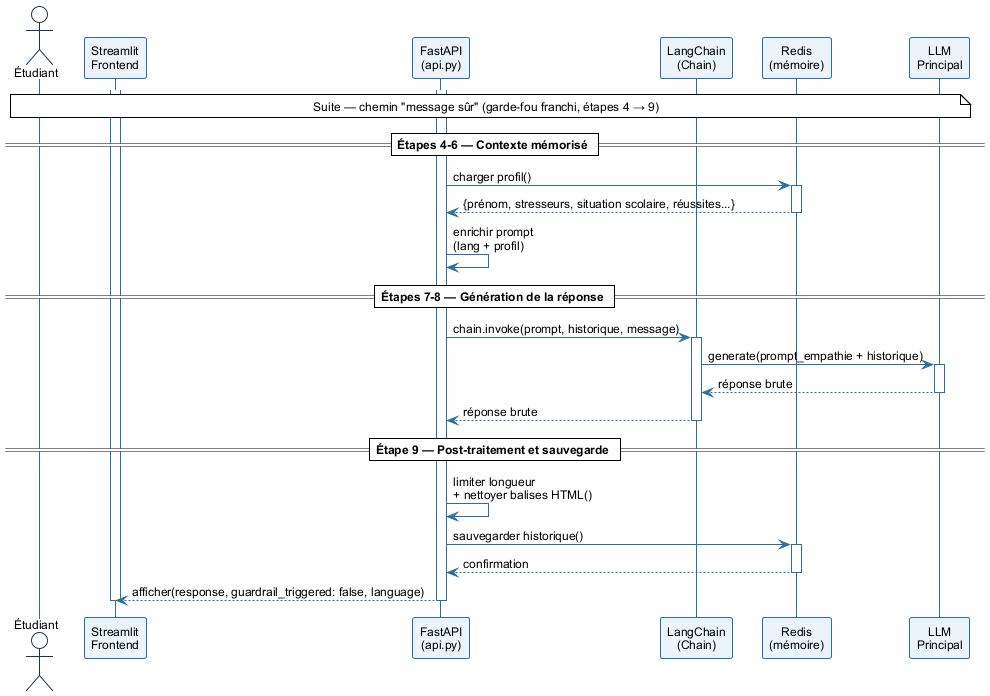
\includegraphics[width=1.15\textwidth]{diagramme/08b_sequence_emotionnel_2.png}
\caption{Diagramme de séquences — Assistant émotionnel (2/2) : génération et sauvegarde}
\label{fig:seq_emotionnel_2}
\end{figure}

\subsection{Diagramme d'activité}

La Figure~\ref{fig:activite_emo} représente le flux de traitement complet
d'un message par l'assistant émotionnel,
depuis la réception jusqu'à la journalisation de l'événement.

\begin{figure}[H]
\centering
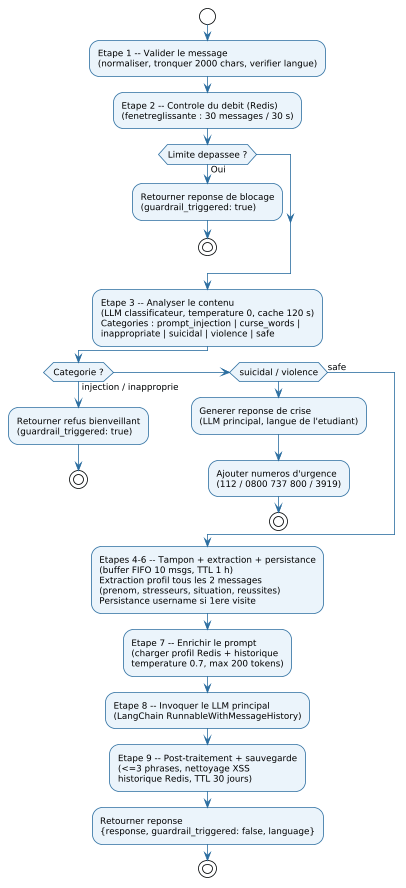
\includegraphics[width=0.6\textwidth]{diagramme/08_activite_emotionnel.png}
\caption{Diagramme d'activité — Assistant émotionnel}
\label{fig:activite_emo}
\end{figure}

% ─────────────────────────────────────────────────────────────────────────────
\section{Module 4 — Classificateur}

\subsection{Conception générale}

Le classificateur de harcèlement est un système d'analyse automatique des textes
soumis à la plateforme Netethic.
Sa conception repose sur la comparaison de quatre stratégies exécutées en parallèle,
permettant d'identifier la plus adaptée selon le type de texte et les conditions d'exécution.

\textbf{Modèle seul.}
Inférence directe du LLM sans contexte additionnel.
Approche généraliste et rapide, servant de référence de comparaison.

\textbf{Modèle avec ancrage juridique.}
Les passages de loi les plus pertinents sont récupérés depuis ChromaDB et injectés
dans la requête, ancrant la décision dans le droit français sur le harcèlement.

\textbf{Règles heuristiques.}
Correspondance par mots-clés spécifiques au français, sans recours au LLM.
Sert de mécanisme de repli rapide en cas d'indisponibilité du modèle.

\textbf{Hybride.}
Appel au LLM avec repli automatique sur les heuristiques en cas d'échec ou d'ambiguïté.
Cette stratégie combine la richesse sémantique du LLM et la robustesse des règles.

\subsection{Diagramme de composants}

La Figure~\ref{fig:composants_classificateur} illustre l'architecture interne du classificateur et la distribution des quatre stratégies de classification.

\begin{figure}[H]
\centering
\hspace*{-0.1\textwidth}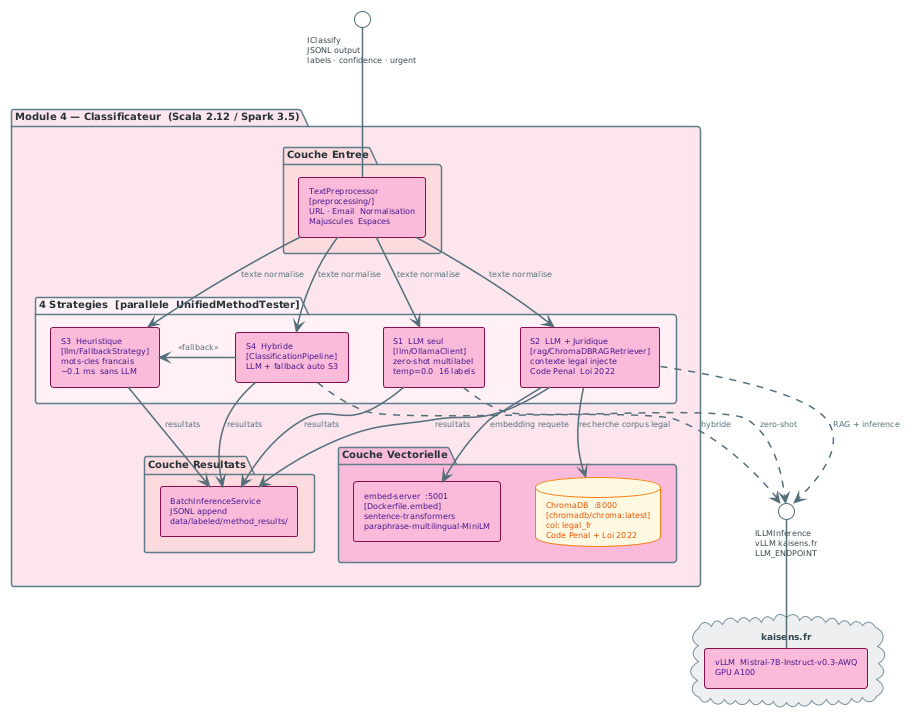
\includegraphics[width=1.2\textwidth]{diagramme/21_composants_classificateur.png}
\caption{Diagramme de composants — Classificateur de harcèlement}
\label{fig:composants_classificateur}
\end{figure}

\subsection{Diagramme de déploiement}

La Figure~\ref{fig:deploiement_classificateur} présente la stack Docker Compose du classificateur avec ses services et leurs interactions.

\begin{figure}[H]
\centering
\hspace*{-0.1\textwidth}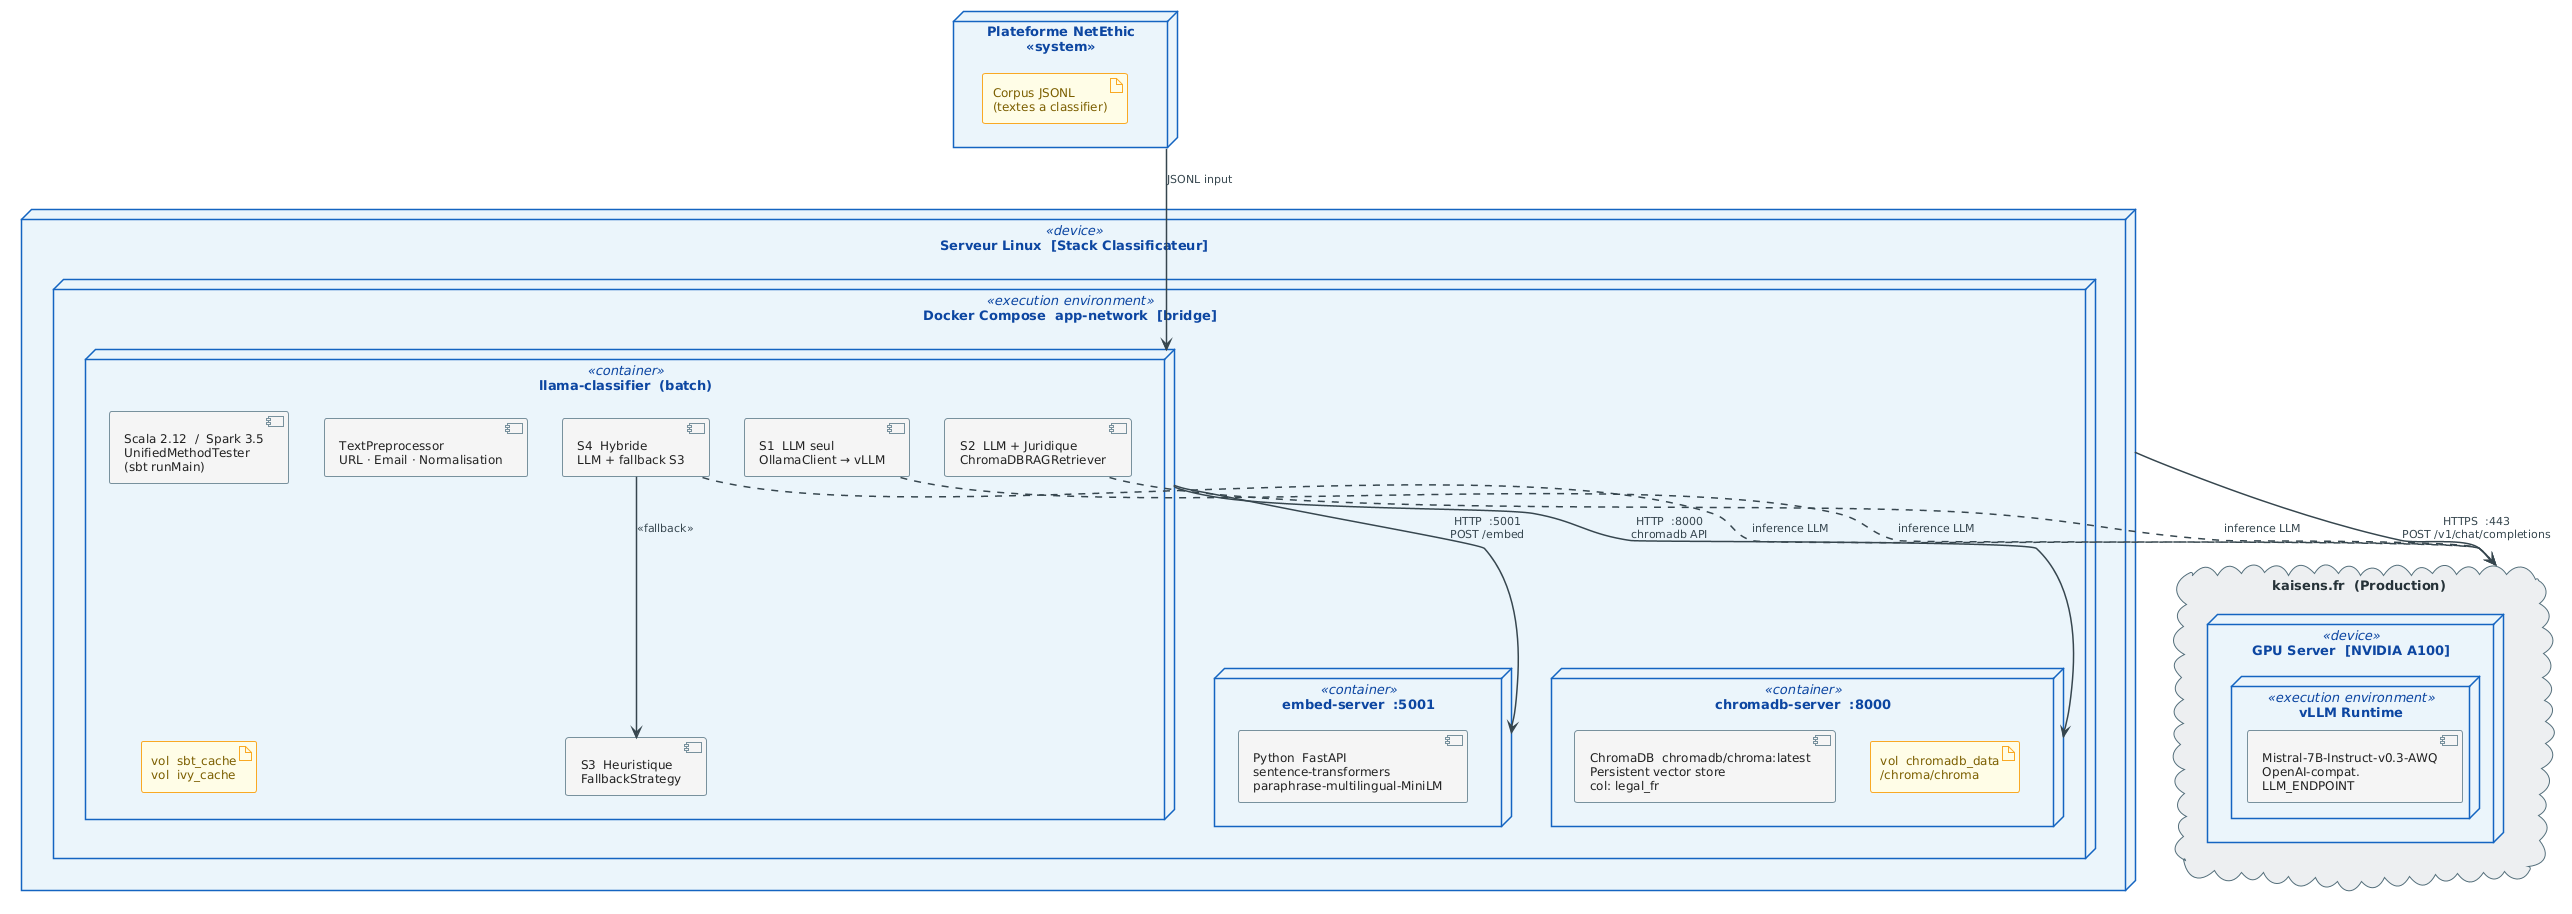
\includegraphics[width=1.2\textwidth]{diagramme/17_deploiement_classificateur.png}
\caption{Diagramme de déploiement — Classificateur de harcèlement (stack Docker Compose)}
\label{fig:deploiement_classificateur}
\end{figure}

\subsection{Diagramme de séquences}

La Figure~\ref{fig:seq_classif} illustre le flux de classification d'un texte.

\begin{figure}[H]
\centering
\hspace*{-0.1\textwidth}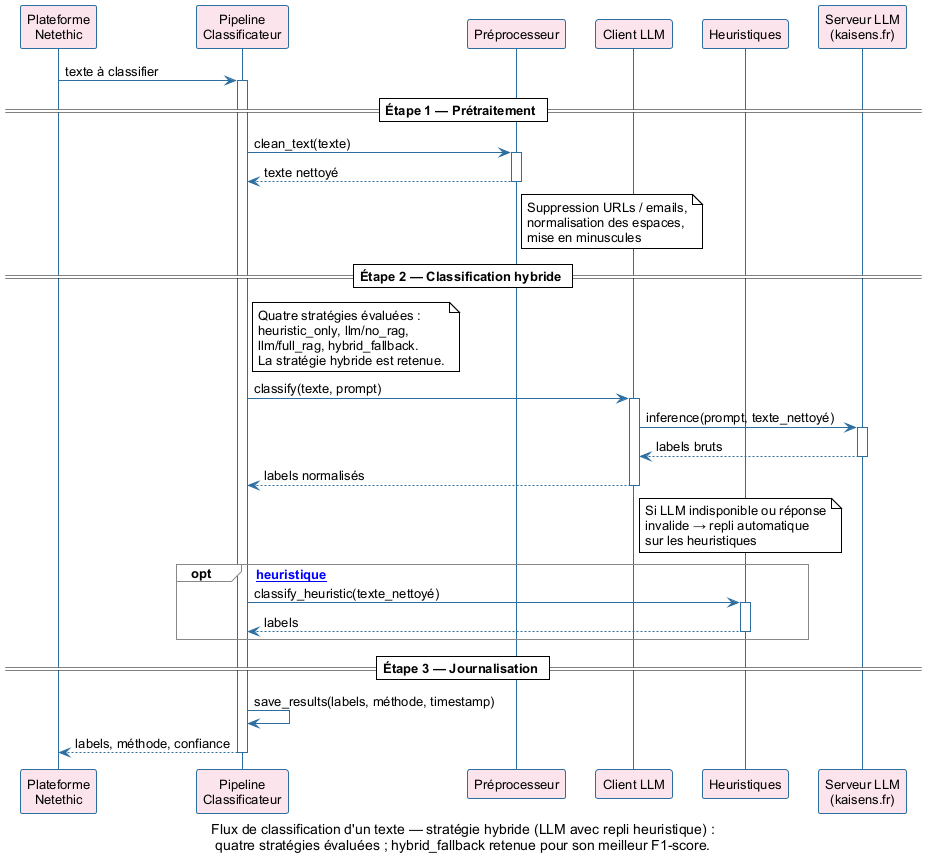
\includegraphics[width=1.2\textwidth]{diagramme/09_sequence_classificateur.png}
\caption{Diagramme de séquences — Classificateur de harcèlement}
\label{fig:seq_classif}
\end{figure}

\subsection{Diagramme d'activité}

La Figure~\ref{fig:activite_classif} représente le flux de traitement complet,
incluant les mécanismes de repli en cas d'échec.

\begin{figure}[H]
\centering
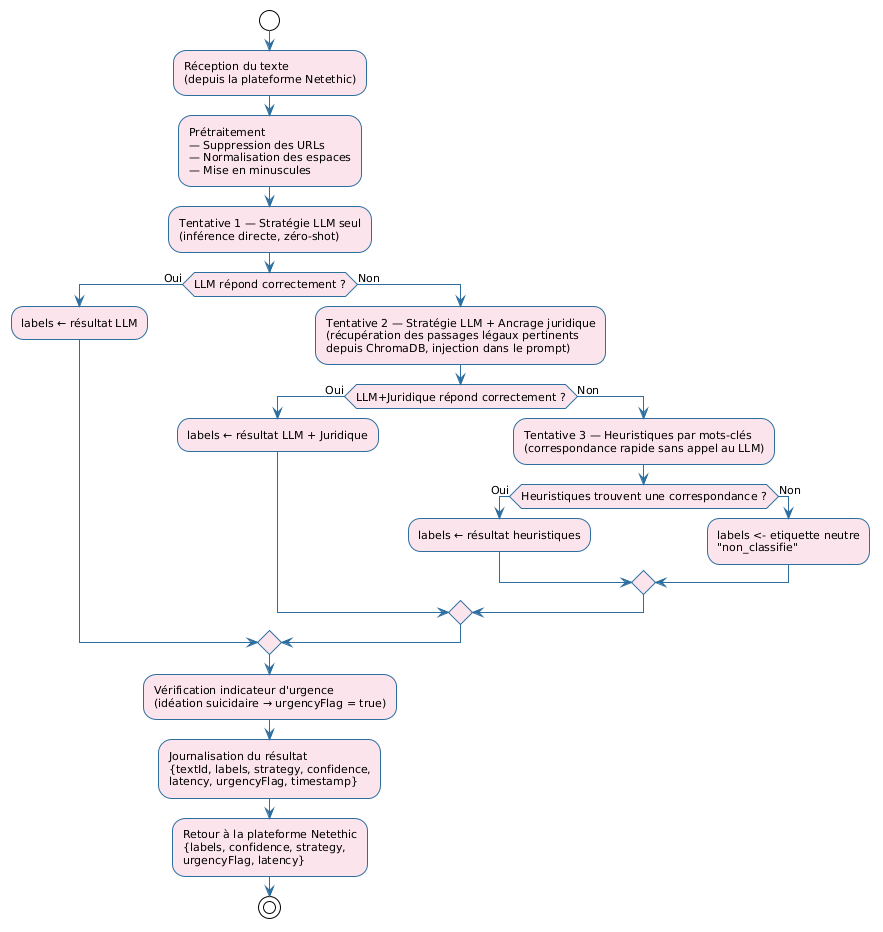
\includegraphics[width=0.95\textwidth]{diagramme/10_activite_classificateur.png}
\caption{Diagramme d'activité — Classificateur (chaîne de repli)}
\label{fig:activite_classif}
\end{figure}

% ─────────────────────────────────────────────────────────────────────────────
\section{Diagramme de classes (Application)}

Le diagramme de classes de la Figure~\ref{fig:classes_app} représente la structure statique
de l'application, c'est-à-dire les entités principales du système, leurs attributs et
les relations qui les unissent.

Les classes centrales sont les suivantes :

\begin{itemize}
    \item \textbf{ChatSession :} Représente une session conversationnelle.
          Attributs : \texttt{sessionId}, \texttt{userId}, \texttt{moduleType}, \texttt{createdAt}, \texttt{expiresAt}.
          Une session agrège plusieurs instances de \texttt{Message}.
    \item \textbf{Message :} Représente un message échangé au cours d'une session.
          Attributs : \texttt{messageId}, \texttt{content}, \texttt{role} (utilisateur/assistant), \texttt{timestamp}.
          Chaque message est associé à une \texttt{IntentClassification} et peut référencer un \texttt{Response}.
    \item \textbf{IntentClassification :} Encapsule le résultat de la classification d'intention.
          Attributs : \texttt{intent} (factual, chitchat, follow-up, forbidden), \texttt{confidence}.
    \item \textbf{DocumentChunk :} Représente un extrait de document indexé dans la base vectorielle.
          Attributs : \texttt{chunkId}, \texttt{content}, \texttt{embedding}, \texttt{category}, \texttt{sourceDocument}.
    \item \textbf{Response :} Encapsule la réponse générée par le LLM.
          Attributs : \texttt{responseId}, \texttt{content}, \texttt{sourceChunks}, \texttt{latency}, \texttt{cached}.
    \item \textbf{ReservationRequest :} Modélise une demande de réservation collectée par l'assistant Noa ou l'assistant technique.
          Attributs : \texttt{requestId}, \texttt{email}, \texttt{phone}, \texttt{requestedDate}, \texttt{channel}, \texttt{subject}.
    \item \textbf{HarassmentClassification :} Encapsule le résultat de l'analyse d'un texte par le classificateur.
          Attributs : \texttt{textId}, \texttt{labels}, \texttt{strategy}, \texttt{confidence}, \texttt{urgencyFlag}, \texttt{timestamp}.
    \item \textbf{EmotionalSignal :} Représente un signal de détresse détecté dans un message.
          Attributs : \texttt{signalType} (dépression, idéation suicidaire, solitude, anxiété, colère, addiction),
          \texttt{severity}, \texttt{detectedAt}.
\end{itemize}

\begin{figure}[H]
\centering
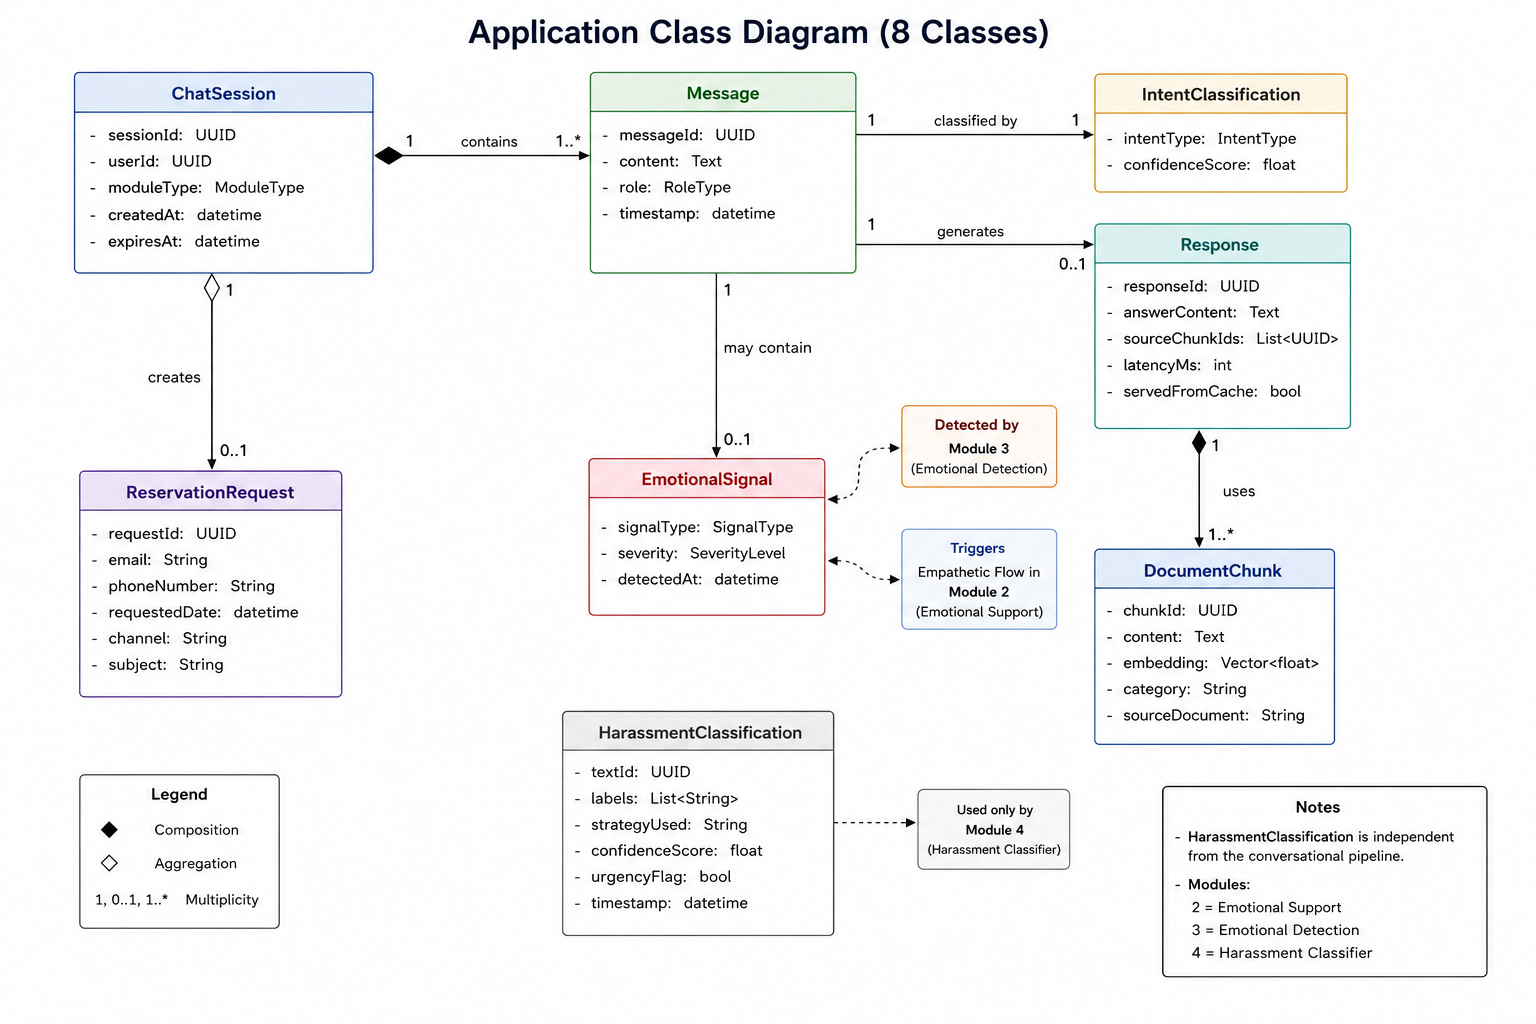
\includegraphics[width=0.95\textwidth]{diagramme/11_classes_application.png}
\caption{Diagramme de classes --- Architecture de l'application}
\label{fig:classes_app}
\end{figure}

% ─────────────────────────────────────────────────────────────────────────────
% PARTIE 2 — Mise en place du modèle d'IA générative
% ─────────────────────────────────────────────────────────────────────────────

\section{Préparation des bases de connaissances RAG}

Les modules assistant Noa et assistant technique reposent sur une architecture
\textit{Retrieval-Augmented Generation} (RAG) dont la qualité des réponses
dépend directement de la qualité et de la structure des documents indexés.
La phase de préparation consiste à transformer les sources documentaires brutes
en fichiers Markdown structurés et enrichis, exploitables par la base
vectorielle ChromaDB.

\subsection{Assistant Noa — sources documentaires publiques}

\paragraph{Extraction et conversion}\mbox{}\newline

La base de connaissances de Noa est constituée à partir du contenu du site public
de Netethic.
Les vingt-et-une pages du site ont été extraites et converties au format Markdown.
Cette conversion produit des fichiers textuels structurés,
plus adaptés au découpage en segments que les sources HTML brutes.

\paragraph{Enrichissement des fichiers Markdown}\mbox{}\newline

Après conversion, chaque fichier Markdown a été relu et enrichi
pour corriger les problèmes courants liés à l'extraction automatique~:

\begin{itemize}
    \item \textbf{Clarification des sous-titres :} Les intitulés de section trop courts
          ou ambigus ont été reformulés pour décrire explicitement le contenu
          de la rubrique et améliorer la précision de la recherche par similarité.
    \item \textbf{Complétion des informations manquantes :} Certains passages
          incomplets (tarifs, conditions d'accès, coordonnées) ont été complétés
          à partir des sources officielles.
    \item \textbf{Suppression des éléments non informatifs :} Les menus de navigation,
          pieds de page et formulaires ont été retirés pour ne conserver
          que le contenu textuel utile à la réponse.
\end{itemize}

\paragraph{Stratégie d'indexation parent-enfant}\mbox{}\newline

Les documents enrichis ont été découpés selon une stratégie parent-enfant~:
les segments courts (enfants) servent à la recherche par similarité sémantique,
tandis que les segments longs (parents) sont transmis au LLM pour générer
une réponse contextuellement riche.
Cette stratégie permet d'allier précision de la recherche et richesse
du contexte fourni au modèle de génération.

Le Tableau~\ref{tab:kb_noa} présente les statistiques de la base de connaissances
constituée pour Noa.

\vspace{6pt}
\begin{table}[H]
\centering
\caption{Statistiques de la base de connaissances — Assistant Noa}
\label{tab:kb_noa}
\begin{tabular}{|l|c|}
\hline
\textbf{Paramètre} & \textbf{Valeur} \\
\hline
Nombre de pages indexées    & 21 \\
\hline
Nombre de segments (chunks) & 177 \\
\hline
Modèle d'embedding          & \texttt{paraphrase-multilingual-mpnet-base-v2} \\
\hline
Seuil de pertinence         & 0,35 \\
\hline
Base vectorielle            & ChromaDB \\
\hline
\end{tabular}
\end{table}

\subsection{Assistant technique — documentation interne}

\paragraph{Sources documentaires}\mbox{}\newline

La base de connaissances de l'assistant technique est constituée à partir
de la documentation technique interne fournie par Smart-Conseil.
Elle couvre les onze catégories fonctionnelles de la plateforme Netethic~:
gestion des utilisateurs, paramétrage, tableaux de bord, rapports, notifications,
intégration, sécurité, conformité RGPD, support technique, administration
et facturation.

\paragraph{Transformation et structuration}\mbox{}\newline

Les documents fournis au format PDF ont été convertis au format Markdown.
Chaque fichier Markdown a ensuite été structuré par catégorie fonctionnelle,
en suivant le même processus d'enrichissement que pour la base de Noa~:
clarification des sous-titres, complétion des informations manquantes
et suppression des éléments non informatifs.

La collection ChromaDB de l'assistant technique est organisée en onze sous-collections,
une par catégorie fonctionnelle.
Cette organisation permet un filtrage précis lors de la recherche vectorielle~:
lorsqu'une catégorie est sélectionnée par l'utilisateur, la recherche
est restreinte aux documents de cette catégorie uniquement,
ce qui améliore la pertinence des résultats retournés.

% ─────────────────────────────────────────────────────────────────────────────
\section{Mise en place du classificateur de harcèlement}

Le classificateur de harcèlement est le module dont la mise en place
diffère fondamentalement des modules conversationnels~:
il ne repose pas sur un pipeline RAG mais sur un cycle complet
d'apprentissage automatique, depuis la collecte des données
jusqu'à l'évaluation comparative des stratégies de classification.

\subsection{Collecte des données}

Le corpus d'expérimentation est constitué de \textbf{977 textes multilingues}
(français et anglais), issus d'une application mobile de modération de contenu.
Tous les textes sont initialement étiquetés \textit{négatif} par l'application.
Le Tableau~\ref{tab:corpus_classif} décrit les caractéristiques du jeu de données brut.

\vspace{6pt}
\begin{table}[H]
\centering
\caption{Caractéristiques du corpus brut — Classificateur de harcèlement}
\label{tab:corpus_classif}
\small
\begin{tabular}{|l|l|}
\hline
\textbf{Caractéristique} & \textbf{Valeur} \\
\hline
Nombre de textes        & 977 \\
\hline
Langues                 & Français et anglais (mélangés) \\
\hline
Source                  & Application mobile de modération de contenu \\
\hline
Encodage                & Latin-1 (ISO-8859-1) \\
\hline
Étiquette initiale      & \textit{negative} (classification de l'application) \\
\hline
\end{tabular}
\end{table}

\subsection{Nettoyage et prétraitement}

L'analyse du corpus a révélé cinq catégories de bruits textuels~:
entités HTML (8 occurrences), images Markdown (3),
textes dépassant 128~caractères (152),
mentions d'utilisateurs (14) et URLs (5).

Un pipeline de prétraitement en cinq étapes a été développé pour normaliser
les textes avant inférence.
Le Tableau~\ref{tab:preprocessing_steps} décrit chaque étape.

\vspace{6pt}
\begin{table}[H]
\centering
\caption{Pipeline de prétraitement du corpus}
\label{tab:preprocessing_steps}
\small
\setlength{\tabcolsep}{4pt}
\begin{tabular}{|c|p{4cm}|p{8cm}|}
\hline
\textbf{Étape} & \textbf{Traitement} & \textbf{Description} \\
\hline
1 & Décodage HTML
  & Conversion des entités HTML (\texttt{\&amp;}, \texttt{\&\#39;}, etc.)
    en caractères lisibles. \\
\hline
2 & Suppression des balises
  & Élimination des balises HTML résiduelles (\texttt{<br>}, \texttt{<a href=...>}, etc.). \\
\hline
3 & Normalisation des mentions
  & Remplacement de toutes les mentions d'utilisateurs par un jeton générique. \\
\hline
4 & Normalisation des URLs
  & Remplacement de toutes les URLs par un jeton générique. \\
\hline
5 & Normalisation des espaces
  & Suppression des sauts de ligne multiples et collapsage des espaces superflus. \\
\hline
\end{tabular}
\end{table}

Le prétraitement conserve l'intégralité des 977~textes (aucune ligne vide
après nettoyage) et ne modifie que 2~prédictions sur 977 (0,2\,\%),
confirmant que les erreurs observées sont intrinsèques au modèle
et non aux données brutes.

\subsection{Augmentation des données}

Le corpus initial présente un déséquilibre de classes~:
après la phase de labeling (voir Section~\ref{subsec:labeling}),
647~textes sont confirmés dans la catégorie négative contre 330~textes
reclassifiés dans des catégories positives ou neutres.
Pour atténuer ce déséquilibre et améliorer la robustesse du modèle,
une stratégie d'augmentation des données a été appliquée à la classe minoritaire.

L'augmentation repose sur la paraphrase automatique par LLM~:
chaque texte de la classe minoritaire est soumis au modèle indépendant
avec une instruction de paraphrase, produisant une version reformulée
sémantiquement équivalente mais lexicalement différente.
Cette technique élargit la diversité des exemples d'entraînement
sans nécessiter de collecte de nouvelles données.

\subsection{Stratégie de labeling — LLM comme juge indépendant}
\label{subsec:labeling}

Pour évaluer la qualité des étiquettes produites par le modèle de classification
initial, une stratégie de \textit{LLM-as-a-Judge} a été adoptée~:
les 977~textes sont soumis à un modèle indépendant (\textbf{Groq API},
modèle \texttt{llama-3.1-8b-instant}) pour obtenir une annotation de référence.

Cette approche évite l'évaluation circulaire dans laquelle un modèle validerait
ses propres prédictions — biais qui rendrait les métriques sans valeur.

Le Tableau~\ref{tab:labeling_results} présente les résultats obtenus.

\vspace{6pt}
\begin{table}[H]
\centering
\caption{Résultats du labeling indépendant — LLM-as-a-Judge}
\label{tab:labeling_results}
\small
\begin{tabular}{|l|c|}
\hline
\textbf{Métrique} & \textbf{Valeur} \\
\hline
Textes confirmés dans la catégorie négative   & 647 / 977 \\
\hline
Textes reclassifiés (positif ou neutre)       & 330 / 977 \\
\hline
Précision du modèle initial                   & 66,2\,\% \\
\hline
Taux d'accord entre les deux modèles         & 63,4\,\% (619 / 977) \\
\hline
Impact du prétraitement sur les prédictions   & 0,2\,\% (2 / 977) \\
\hline
\end{tabular}
\end{table}

Les 33,8\,\% de désaccords s'expliquent principalement par un écart de domaine~:
le modèle initial a été entraîné sur des données formelles anglophones,
alors que le corpus contient de l'argot jeune francophone
(\og trop sous coter \fg{}, \og le meilleurrrrrr \fg{})
que ce modèle interprète incorrectement comme négatif.

\subsection{Entraînement et optimisation}

Quatre stratégies de classification ont été développées et comparées,
correspondant aux approches définies dans la partie conception de ce chapitre~:

\begin{enumerate}
    \item \textbf{Modèle seul :} Inférence directe du LLM sans contexte additionnel.
          Approche généraliste et rapide, servant de référence de comparaison.

    \item \textbf{Modèle avec ancrage juridique :} Les passages de loi les plus
          pertinents sont récupérés dynamiquement et injectés dans la requête,
          ancrant la décision dans le droit français sur le harcèlement.

    \item \textbf{Règles heuristiques :} Correspondance par mots-clés spécifiques
          au français, sans recours au LLM.
          Sert de mécanisme de repli rapide en cas d'indisponibilité du modèle.

    \item \textbf{Hybride :} Appel au LLM avec repli automatique sur les heuristiques
          en cas d'échec ou d'ambiguïté de la réponse du modèle.
\end{enumerate}

L'implémentation est disponible en deux versions complémentaires~:
\begin{itemize}
    \item \textbf{Version Python :} Adaptée aux expérimentations sur des corpus réduits,
          permettant de tester rapidement les quatre stratégies et de comparer
          leurs résultats avant mise en production.
    \item \textbf{Version Scala/Spark :} Conçue pour le traitement en parallèle
          à grande échelle avec Apache Spark~3.5, distribuant l'analyse sur
          l'ensemble des messages soumis à la plateforme Netethic.
\end{itemize}

\subsection{Évaluation des performances}
\label{subsec:eval_classif}

Le Tableau~\ref{tab:eval_classif} présente les métriques d'évaluation
des quatre stratégies sur le corpus de test.

\vspace{6pt}
\begin{table}[H]
\centering
\caption{Évaluation comparative des quatre stratégies de classification}
\label{tab:eval_classif}
\begin{tabular}{|l|c|c|c|}
\hline
\textbf{Stratégie} & \textbf{Précision} & \textbf{Rappel} & \textbf{F1-score} \\
\hline
Modèle seul                   & 0,295 & 0,437 & 0,352 \\
\hline
Modèle avec ancrage juridique & 0,223 & 0,606 & 0,326 \\
\hline
Règles heuristiques           & —     & —     & —     \\
\hline
Hybride                       & —     & —     & \textbf{0,619} \\
\hline
\end{tabular}
\end{table}

Le corpus de test comprend 1\,500~textes en français couvrant les 16~catégories
de la taxonomie (10~actes de harcèlement et 6~signaux de détresse).
La stratégie hybride atteint le meilleur F1-score global (0,619),
soit une amélioration de~76\,\% par rapport au modèle seul (0,352),
confirmant l'intérêt de combiner l'inférence LLM avec les règles heuristiques
comme mécanisme de repli.
La stratégie avec ancrage juridique améliore le rappel (0,606) au détriment
de la précision (0,223), ce qui traduit une tendance à surclasser les textes
ambigus comme relevant du harcèlement.

% ─────────────────────────────────────────────────────────────────────────────
\section*{Conclusion}

Ce chapitre a couvert la conception du système et la mise en place des modèles d'IA.
La partie conception a présenté l'architecture commune et les diagrammes UML de chaque module.
La mise en place a établi les bases de connaissances RAG (177~segments pour Noa,
11~collections pour l'assistant technique) et validé la stratégie hybride
pour le classificateur avec un F1-score de 0,619 sur 1\,500~textes de test.
Le chapitre suivant présente la réalisation concrète du système, les interfaces développées,
les résultats des tests automatisés et les évaluations de qualité.

\chapter{Mise en place du modèle d'IA générative}

% ─────────────────────────────────────────────────────────────────────────────
\section{Introduction}

Ce chapitre décrit la phase de préparation des données et de mise en place
des modèles d'intelligence artificielle pour chacun des quatre modules du système.

Pour les modules conversationnels fondés sur une architecture RAG —
Noa et le Support Assistant — cette phase consiste en la construction
et l'enrichissement des bases de connaissances documentaires exploitées
lors de la recherche par similarité sémantique.

Pour le classificateur de harcèlement, elle couvre le cycle complet
d'apprentissage automatique : collecte des données, nettoyage et prétraitement,
augmentation, labeling, entraînement et évaluation comparative des stratégies.

Le module de soutien émotionnel, dont l'architecture repose exclusivement sur
l'ingénierie de prompt sans base documentaire ni données d'entraînement,
n'est pas concerné par cette phase.

% ─────────────────────────────────────────────────────────────────────────────
\section{Préparation des bases de connaissances RAG}

Les modules Noa et Support Assistant reposent sur une architecture
\textit{Retrieval-Augmented Generation} (RAG) dont la qualité des réponses
dépend directement de la qualité et de la structure des documents indexés.
La phase de préparation consiste à transformer les sources documentaires brutes
en fichiers Markdown structurés et enrichis, exploitables par la base
vectorielle ChromaDB.

\subsection{Module Noa — sources documentaires publiques}

\subsubsection{Extraction et conversion}

La base de connaissances de Noa est constituée à partir du contenu du site public
de Netethic.
Les vingt-et-une pages du site ont été extraites et converties au format Markdown.
Cette conversion produit des fichiers textuels structurés,
plus adaptés au découpage en segments que les sources HTML brutes.

\subsubsection{Enrichissement des fichiers Markdown}

Après conversion, chaque fichier Markdown a été relu et enrichi
pour corriger les problèmes courants liés à l'extraction automatique~:

\begin{itemize}
    \item \textbf{Clarification des sous-titres :} les intitulés de section trop courts
          ou ambigus ont été reformulés pour décrire explicitement le contenu
          de la rubrique et améliorer la précision de la recherche par similarité.
    \item \textbf{Complétion des informations manquantes :} certains passages
          incomplets (tarifs, conditions d'accès, coordonnées) ont été complétés
          à partir des sources officielles.
    \item \textbf{Suppression des éléments non informatifs :} menus de navigation,
          pieds de page et formulaires ont été retirés pour ne conserver
          que le contenu textuel utile à la réponse.
\end{itemize}

\subsubsection{Stratégie d'indexation parent-enfant}

Les documents enrichis ont été découpés selon une stratégie parent-enfant~:
les segments courts (enfants) servent à la recherche par similarité sémantique,
tandis que les segments longs (parents) sont transmis au LLM pour générer
une réponse contextuellement riche.
Cette stratégie permet d'allier précision de la recherche et richesse
du contexte fourni au modèle de génération.

Le Tableau~\ref{tab:kb_noa} présente les statistiques de la base de connaissances
constituée pour Noa.

\vspace{6pt}
\begin{table}[H]
\centering
\caption{Statistiques de la base de connaissances — Module Noa}
\label{tab:kb_noa}
\begin{tabular}{|l|c|}
\hline
\textbf{Paramètre} & \textbf{Valeur} \\
\hline
Nombre de pages indexées    & 21 \\
\hline
Nombre de segments (chunks) & 177 \\
\hline
Modèle d'embedding          & \texttt{paraphrase-multilingual-mpnet-base-v2} \\
\hline
Seuil de pertinence         & 0,35 \\
\hline
Base vectorielle            & ChromaDB \\
\hline
\end{tabular}
\end{table}

\subsection{Module Support Assistant — documentation interne}

\subsubsection{Sources documentaires}

La base de connaissances du Support Assistant est constituée à partir
de la documentation technique interne fournie par Smart-Conseil.
Elle couvre les onze catégories fonctionnelles de la plateforme Netethic~:
gestion des utilisateurs, paramétrage, tableaux de bord, rapports, notifications,
intégration, sécurité, conformité RGPD, support technique, administration
et facturation.

\subsubsection{Transformation et structuration}

Les documents fournis au format PDF ont été convertis au format Markdown.
Chaque fichier Markdown a ensuite été structuré par catégorie fonctionnelle,
en suivant le même processus d'enrichissement que pour la base de Noa~:
clarification des sous-titres, complétion des informations manquantes
et suppression des éléments non informatifs.

La collection ChromaDB du Support Assistant est organisée en onze sous-collections,
une par catégorie fonctionnelle.
Cette organisation permet un filtrage précis lors de la recherche vectorielle~:
lorsqu'une catégorie est sélectionnée par l'utilisateur, la recherche
est restreinte aux documents de cette catégorie uniquement,
ce qui améliore la pertinence des résultats retournés.

% ─────────────────────────────────────────────────────────────────────────────
\section{Mise en place du classificateur de harcèlement}

Le classificateur de harcèlement est le module dont la mise en place
diffère fondamentalement des modules conversationnels~:
il ne repose pas sur un pipeline RAG mais sur un cycle complet
d'apprentissage automatique, depuis la collecte des données
jusqu'à l'évaluation comparative des stratégies de classification.

\subsection{Collecte des données}

Le corpus d'expérimentation est constitué de \textbf{977 textes multilingues}
(français et anglais), issus d'une application mobile de modération de contenu.
Tous les textes sont initialement étiquetés \textit{négatif} par l'application.
Le Tableau~\ref{tab:corpus_classif} décrit les caractéristiques du jeu de données brut.

\vspace{6pt}
\begin{table}[H]
\centering
\caption{Caractéristiques du corpus brut — Classificateur de harcèlement}
\label{tab:corpus_classif}
\small
\begin{tabular}{|l|l|}
\hline
\textbf{Caractéristique} & \textbf{Valeur} \\
\hline
Nombre de textes        & 977 \\
\hline
Langues                 & Français et anglais (mélangés) \\
\hline
Source                  & Application mobile de modération de contenu \\
\hline
Encodage                & Latin-1 (ISO-8859-1) \\
\hline
Étiquette initiale      & \textit{negative} (classification de l'application) \\
\hline
\end{tabular}
\end{table}

\subsection{Nettoyage et prétraitement}

L'analyse du corpus a révélé cinq catégories de bruits textuels~:
entités HTML (8 occurrences), images Markdown (3),
textes dépassant 128~caractères (152),
mentions d'utilisateurs (14) et URLs (5).

Un pipeline de prétraitement en cinq étapes a été développé pour normaliser
les textes avant inférence.
Le Tableau~\ref{tab:preprocessing_steps} décrit chaque étape.

\vspace{6pt}
\begin{table}[H]
\centering
\caption{Pipeline de prétraitement du corpus}
\label{tab:preprocessing_steps}
\small
\setlength{\tabcolsep}{4pt}
\begin{tabular}{|c|p{4cm}|p{8cm}|}
\hline
\textbf{Étape} & \textbf{Traitement} & \textbf{Description} \\
\hline
1 & Décodage HTML
  & Conversion des entités HTML (\texttt{\&amp;}, \texttt{\&\#39;}, etc.)
    en caractères lisibles. \\
\hline
2 & Suppression des balises
  & Élimination des balises HTML résiduelles (\texttt{<br>}, \texttt{<a href=...>}, etc.). \\
\hline
3 & Normalisation des mentions
  & Remplacement de toutes les mentions d'utilisateurs par un jeton générique. \\
\hline
4 & Normalisation des URLs
  & Remplacement de toutes les URLs par un jeton générique. \\
\hline
5 & Normalisation des espaces
  & Suppression des sauts de ligne multiples et collapsage des espaces superflus. \\
\hline
\end{tabular}
\end{table}

Le prétraitement conserve l'intégralité des 977~textes (aucune ligne vide
après nettoyage) et ne modifie que 2~prédictions sur 977 (0,2\,\%),
confirmant que les erreurs observées sont intrinsèques au modèle
et non aux données brutes.

\subsection{Augmentation des données}

Le corpus initial présente un déséquilibre de classes~:
après la phase de labeling (voir Section~\ref{subsec:labeling}),
647~textes sont confirmés dans la catégorie négative contre 330~textes
reclassifiés dans des catégories positives ou neutres.
Pour atténuer ce déséquilibre et améliorer la robustesse du modèle,
une stratégie d'augmentation des données a été appliquée à la classe minoritaire.

L'augmentation repose sur la paraphrase automatique par LLM~:
chaque texte de la classe minoritaire est soumis au modèle indépendant
avec une instruction de paraphrase, produisant une version reformulée
sémantiquement équivalente mais lexicalement différente.
Cette technique élargit la diversité des exemples d'entraînement
sans nécessiter de collecte de nouvelles données.

\subsection{Stratégie de labeling — LLM comme juge indépendant}
\label{subsec:labeling}

Pour évaluer la qualité des étiquettes produites par le modèle de classification
initial, une stratégie de \textit{LLM-as-a-Judge} a été adoptée~:
les 977~textes sont soumis à un modèle indépendant (\textbf{Groq API},
modèle \texttt{llama-3.1-8b-instant}) pour obtenir une annotation de référence.

Cette approche évite l'évaluation circulaire dans laquelle un modèle validerait
ses propres prédictions — biais qui rendrait les métriques sans valeur.

Le Tableau~\ref{tab:labeling_results} présente les résultats obtenus.

\vspace{6pt}
\begin{table}[H]
\centering
\caption{Résultats du labeling indépendant — LLM-as-a-Judge}
\label{tab:labeling_results}
\small
\begin{tabular}{|l|c|}
\hline
\textbf{Métrique} & \textbf{Valeur} \\
\hline
Textes confirmés dans la catégorie négative   & 647 / 977 \\
\hline
Textes reclassifiés (positif ou neutre)       & 330 / 977 \\
\hline
Précision du modèle initial                   & 66,2\,\% \\
\hline
Taux d'accord entre les deux modèles         & 63,4\,\% (619 / 977) \\
\hline
Impact du prétraitement sur les prédictions   & 0,2\,\% (2 / 977) \\
\hline
\end{tabular}
\end{table}

Les 33,8\,\% de désaccords s'expliquent principalement par un écart de domaine~:
le modèle initial a été entraîné sur des données formelles anglophones,
alors que le corpus contient de l'argot jeune francophone
(\og trop sous coter \fg{}, \og le meilleurrrrrr \fg{})
que ce modèle interprète incorrectement comme négatif.

\subsection{Entraînement et optimisation}

Quatre stratégies de classification ont été développées et comparées,
correspondant aux approches définies lors de la conception (Chapitre~4)~:

\begin{enumerate}
    \item \textbf{Modèle seul :} inférence directe du LLM sans contexte additionnel.
          Approche généraliste et rapide, servant de référence de comparaison.

    \item \textbf{Modèle avec ancrage juridique :} les passages de loi les plus
          pertinents sont récupérés dynamiquement et injectés dans la requête,
          ancrant la décision dans le droit français sur le harcèlement.

    \item \textbf{Règles heuristiques :} correspondance par mots-clés spécifiques
          au français, sans recours au LLM.
          Sert de mécanisme de repli rapide en cas d'indisponibilité du modèle.

    \item \textbf{Hybride :} appel au LLM avec repli automatique sur les heuristiques
          en cas d'échec ou d'ambiguïté de la réponse du modèle.
\end{enumerate}

L'implémentation est disponible en deux versions complémentaires~:
\begin{itemize}
    \item \textbf{Version Python :} adaptée aux expérimentations sur des corpus réduits,
          permettant de tester rapidement les quatre stratégies et de comparer
          leurs résultats avant mise en production.
    \item \textbf{Version Scala/Spark :} conçue pour le traitement en parallèle
          à grande échelle avec Apache Spark~3.5, distribuant l'analyse sur
          l'ensemble des messages soumis à la plateforme Netethic.
\end{itemize}

\subsection{Évaluation des performances}
\label{subsec:eval_classif}

L'évaluation comparative a été conduite en deux temps~:
une première évaluation globale sur le corpus Scala/Spark (1\,500~textes,
16~catégories), puis une évaluation ciblée sur un \textbf{échantillon stratifié}
de 150~textes (50~par classe~: Harcèlement, Santé mentale, Non-harcèlement)
afin d'obtenir des métriques équilibrées, non biaisées par la distribution
naturelle des classes.

\subsubsection*{Résultats globaux — pipeline Scala/Spark}

Le Tableau~\ref{tab:eval_classif} présente les métriques d'évaluation
des quatre stratégies sur le corpus de test de 1\,500~textes.

\vspace{6pt}
\begin{table}[H]
\centering
\caption{Évaluation comparative des stratégies — corpus Scala/Spark (1\,500 textes)}
\label{tab:eval_classif}
\begin{tabular}{|l|c|c|c|}
\hline
\textbf{Stratégie} & \textbf{Précision} & \textbf{Rappel} & \textbf{F1-score} \\
\hline
Modèle seul                   & 0{,}295 & 0{,}437 & 0{,}352 \\
\hline
Modèle avec ancrage juridique & 0{,}223 & 0{,}606 & 0{,}326 \\
\hline
Règles heuristiques           & 0{,}110 & 0{,}333 & 0{,}167 \\
\hline
Hybride                       & 0{,}631 & 0{,}607 & \textbf{0{,}619} \\
\hline
\end{tabular}
\end{table}

La stratégie hybride atteint le meilleur F1-score global (0{,}619),
soit une amélioration de~76\,\% par rapport au modèle seul (0{,}352).
La stratégie avec ancrage juridique améliore le rappel (0{,}606) au détriment
de la précision (0{,}223), traduisant une tendance à surclasser les textes
ambigus comme relevant du harcèlement.
Les règles heuristiques, en classant la quasi-totalité des textes dans la
catégorie Non-harcèlement, obtiennent un F1-score macro de 0{,}167 ~:
elles ne constituent qu'un mécanisme de repli et non une stratégie principale.

\subsubsection*{Évaluation ciblée — pipeline Python LLM (échantillon stratifié)}

Pour valider le comportement du pipeline Python sur les trois classes cibles
de la plateforme Netethic, une évaluation sur un \textbf{échantillon stratifié
de 150~textes} (50~par classe) a été conduite sur \textbf{cinq configurations}~:
la ligne de base heuristique, deux variantes du prompt RAG binaire (sans et avec
RAG juridique), et deux variantes du prompt Multilabel (sans et avec RAG).

\vspace{6pt}
\begin{table}[H]
\centering
\caption{Évaluation sur échantillon stratifié — pipeline Python LLM (150 textes, 50/classe)}
\label{tab:eval_python}
\small
\begin{tabular}{|l|l|c|c|c|}
\hline
\textbf{Stratégie} & \textbf{Classe} & \textbf{Précision} & \textbf{Rappel} & \textbf{F1-score} \\
\hline
\multirow{4}{*}{Règles heuristiques}
 & Harcèlement      & 0{,}00 & 0{,}00 & 0{,}00 \\
 & Santé mentale    & 0{,}00 & 0{,}00 & 0{,}00 \\
 & Non-harcèlement  & 0{,}33 & 1{,}00 & 0{,}50 \\
 & \textit{Macro}   & \textit{0{,}11} & \textit{0{,}33} & \textit{0{,}17} \\
\hline
\multirow{3}{*}{RAG-prompt (sans RAG)}
 & Harcèlement      & 0{,}69 & 0{,}70 & 0{,}69 \\
 & Santé mentale    & --- & --- & --- \\
 & Non-harcèlement  & 0{,}43 & 0{,}86 & 0{,}58 \\
 & \textit{Macro}   & \textit{0{,}37} & \textit{0{,}52} & \textit{0{,}42} \\
\hline
\multirow{3}{*}{RAG-prompt (avec RAG)}
 & Harcèlement      & 0{,}73 & 0{,}76 & 0{,}75 \\
 & Santé mentale    & --- & --- & --- \\
 & Non-harcèlement  & 0{,}45 & 0{,}88 & 0{,}59 \\
 & \textit{Macro}   & \textit{0{,}39} & \textit{0{,}55} & \textit{0{,}45} \\
\hline
\multirow{4}{*}{Multilabel LLM (sans RAG)}
 & Harcèlement      & 0{,}51 & 0{,}74 & 0{,}61 \\
 & Santé mentale    & \textbf{0{,}94} & 0{,}34 & 0{,}50 \\
 & Non-harcèlement  & 0{,}53 & 0{,}64 & 0{,}58 \\
 & \textit{Macro}   & \textit{0{,}66} & \textit{0{,}57} & \textit{0{,}56} \\
\hline
\multirow{4}{*}{\textbf{Multilabel LLM (avec RAG)}}
 & Harcèlement      & \textbf{0{,}68} & \textbf{0{,}76} & \textbf{0{,}72} \\
 & Santé mentale    & 0{,}71 & 0{,}40 & 0{,}51 \\
 & Non-harcèlement  & \textbf{0{,}55} & 0{,}72 & \textbf{0{,}62} \\
 & \textit{Macro}   & \textit{0{,}65} & \textit{0{,}63} & \textbf{\textit{0{,}62}} \\
\hline
\end{tabular}
\end{table}

\noindent\textit{Note~: le prompt RAG binaire prédit uniquement deux classes
(Harcèlement / Non-harcèlement)~; la Santé mentale est absente de sa taxonomie (---).}

La Figure~\ref{fig:eval_classif_comparison} illustre graphiquement
la comparaison entre les cinq stratégies sur les trois dimensions d'évaluation.

\begin{figure}[H]
\centering
\includegraphics[width=\textwidth]{figures/eval_classif_comparison.pdf}
\caption{Comparaison des cinq stratégies de classification~: métriques globales
         (F1 macro, accuracy), F1 par classe, et précision/rappel pour les
         classes Harcèlement et Santé mentale.
         Échantillon stratifié de 150~textes (50 par classe).}
\label{fig:eval_classif_comparison}
\end{figure}

La configuration \textbf{Multilabel LLM avec RAG} obtient le meilleur F1 macro
(\textbf{0{,}62}) et la meilleure exactitude (\textbf{63{,}0\,\%}),
confirmant l'apport combiné du prompt taxonomique et de l'ancrage RAG juridique.
Le prompt RAG binaire, bien qu'il atteigne un F1 de 0{,}75 sur la classe
Harcèlement avec RAG, ne peut structurellement pas détecter la Santé mentale,
ce qui pénalise son F1 macro (0{,}45).
L'analyse par classe pour la meilleure configuration révèle~:
\begin{itemize}
    \item \textbf{Harcèlement~:} rappel de \textbf{0{,}76} et F1 de 0{,}72 —
          le modèle détecte les trois quarts des cas avec une précision de 0{,}68,
          améliorée grâce aux exemples légaux récupérés par le RAG.
    \item \textbf{Santé mentale~:} précision de 0{,}71 et rappel de 0{,}40 —
          les signaux de détresse sont correctement identifiés lorsque détectés~;
          le rappel modéré reflète la difficulté à distinguer les expressions
          émotionnelles subtiles.
    \item \textbf{Non-harcèlement~:} F1 de \textbf{0{,}62} avec un rappel de 0{,}72 —
          le modèle reconnaît correctement la majorité des échanges neutres,
          limitant les faux positifs sur les conversations anodines.
\end{itemize}
Ces résultats valident l'architecture Multilabel LLM avec RAG comme stratégie
optimale pour la détection tripartite du harcèlement en ligne au sein de la
plateforme Netethic.

% ─────────────────────────────────────────────────────────────────────────────
\section{Conclusion}

Ce chapitre a présenté la phase de préparation des données et de mise en place
des modèles d'intelligence artificielle pour les quatre modules du système.

Pour les modules conversationnels, la qualité des réponses repose directement
sur la qualité des bases de connaissances~: les vingt-et-une pages publiques
de Netethic ont été transformées en 177~segments structurés selon une stratégie
parent-enfant pour Noa, et les documents du Support Assistant ont été organisés
en onze collections correspondant aux catégories fonctionnelles de la plateforme.
Dans les deux cas, un enrichissement manuel des fichiers Markdown — clarification
des sous-titres et complétion des informations manquantes — a permis d'améliorer
la pertinence des résultats de recherche vectorielle.

Pour le classificateur de harcèlement, le cycle d'apprentissage complet —
collecte de 977~textes, nettoyage en cinq étapes, augmentation par paraphrase
automatique, labeling indépendant et comparaison de quatre stratégies —
a abouti à un F1-score de 0{,}619 pour la stratégie hybride sur le corpus
Scala/Spark, contre 0{,}352 pour le modèle seul.
L'évaluation ciblée du pipeline Python LLM sur échantillon stratifié confirme
la supériorité de l'approche Multilabel LLM avec RAG (F1 macro \textbf{0{,}62})
sur toutes les autres configurations, dont le prompt RAG binaire (0{,}45) et la
ligne de base heuristique (0{,}17), avec des F1-scores de 0{,}72 sur Harcèlement,
0{,}51 sur Santé mentale et 0{,}62 sur Non-harcèlement.

Le chapitre suivant présente la réalisation concrète du système~:
interfaces utilisateur, résultats des tests automatisés, mesures de sécurité
et optimisations de performance.

\chapter{Réalisation et tests}

% ─────────────────────────────────────────────────────────────────────────────
\section{Introduction}

Ce chapitre présente la phase de réalisation du système et les résultats obtenus.
La préparation des données et la mise en place des modèles d'IA ayant été traitées
au Chapitre~5, ce chapitre couvre l'environnement de développement,
les interfaces réalisées, les tests effectués,
les aspects de sécurité selon le référentiel OWASP Top~10 for LLM Applications,
l'évaluation de la qualité des réponses avec le framework RAGAS,
les optimisations de performance et le déploiement.

% ─────────────────────────────────────────────────────────────────────────────
\section{Environnement de développement}

\subsection{Environnement matériel et logiciel}

Le développement a été réalisé sur des machines sous Windows~11 avec accès au serveur
d'inférence kaisens.fr.
Le Tableau~\ref{tab:env_dev} présente les outils et technologies utilisés.

\vspace{6pt}
\begin{table}[H]
\centering
\caption{Environnement de développement}
\label{tab:env_dev}
\begin{tabular}{|l|l|}
\hline
\textbf{Catégorie} & \textbf{Outil / Version} \\
\hline
Langage principal & Python 3.11 \\
Langage traitement de données & Scala 2.12.18 / Apache Spark 3.5 \\
Interface interne & Streamlit 1.32 \\
Interface publique & React 18 + Vite \\
Backend API & FastAPI 0.110 \\
Orchestration LLM & LangChain 0.2 \\
Base documentaire & ChromaDB 0.5 \\
Mémoire de session & Redis 7.2 \\
Évaluation RAG & RAGAS 0.1 (juge LLM : Groq API) \\
Conteneurisation & Docker / Docker Compose \\
Contrôle de version & Git / GitLab (\texttt{gitlab.dataforethic.fr}) \\
\hline
\end{tabular}
\end{table}

% ─────────────────────────────────────────────────────────────────────────────
\section{Module 1 — Noa : assistant virtuel du site public}

\subsection{Tests}

Une suite de 46~tests automatisés couvre l'ensemble des fonctionnalités de Noa.
Le Tableau~\ref{tab:tests_noa} présente les résultats obtenus.

\vspace{6pt}
\begin{table}[H]
\centering
\caption{Résultats des tests automatisés — Module Noa}
\label{tab:tests_noa}
\begin{tabular}{|l|c|c|}
\hline
\textbf{Catégorie de test} & \textbf{Nombre} & \textbf{Résultat} \\
\hline
Routage par intention & 8 & 100\,\% \\
Recherche documentaire & 10 & 100\,\% \\
Agent de réservation & 12 & 100\,\% \\
Mémoire et cache & 8 & 100\,\% \\
Gestion des erreurs & 8 & 100\,\% \\
\hline
\textbf{Total} & \textbf{46} & \textbf{100\,\%} \\
\hline
\end{tabular}
\end{table}

\subsection{Performances}

Le Tableau~\ref{tab:perf_noa} présente les temps de réponse mesurés pour chaque type de requête.

\vspace{6pt}
\begin{table}[H]
\centering
\caption{Temps de réponse moyens — Module Noa}
\label{tab:perf_noa}
\begin{tabular}{|l|c|c|}
\hline
\textbf{Type de requête} & \textbf{Temps moyen} & \textbf{Exigence} \\
\hline
Réponse depuis le cache & $<$ 1\,ms & $<$ 50\,ms \\
Salutation / hors sujet & $<$ 10\,ms & $<$ 100\,ms \\
Question factuelle (RAG) & $\approx$ 1,8\,s & $<$ 5\,s \\
Question de suivi & $\approx$ 2,1\,s & $<$ 5\,s \\
\hline
\end{tabular}
\end{table}

% ─────────────────────────────────────────────────────────────────────────────
\section{Module 2 — NetEthic Support Assistant}

\subsection{Interface utilisateur}

La Figure~\ref{fig:support_interface} montre l'interface principale du Support Assistant.

\begin{figure}[H]
\centering
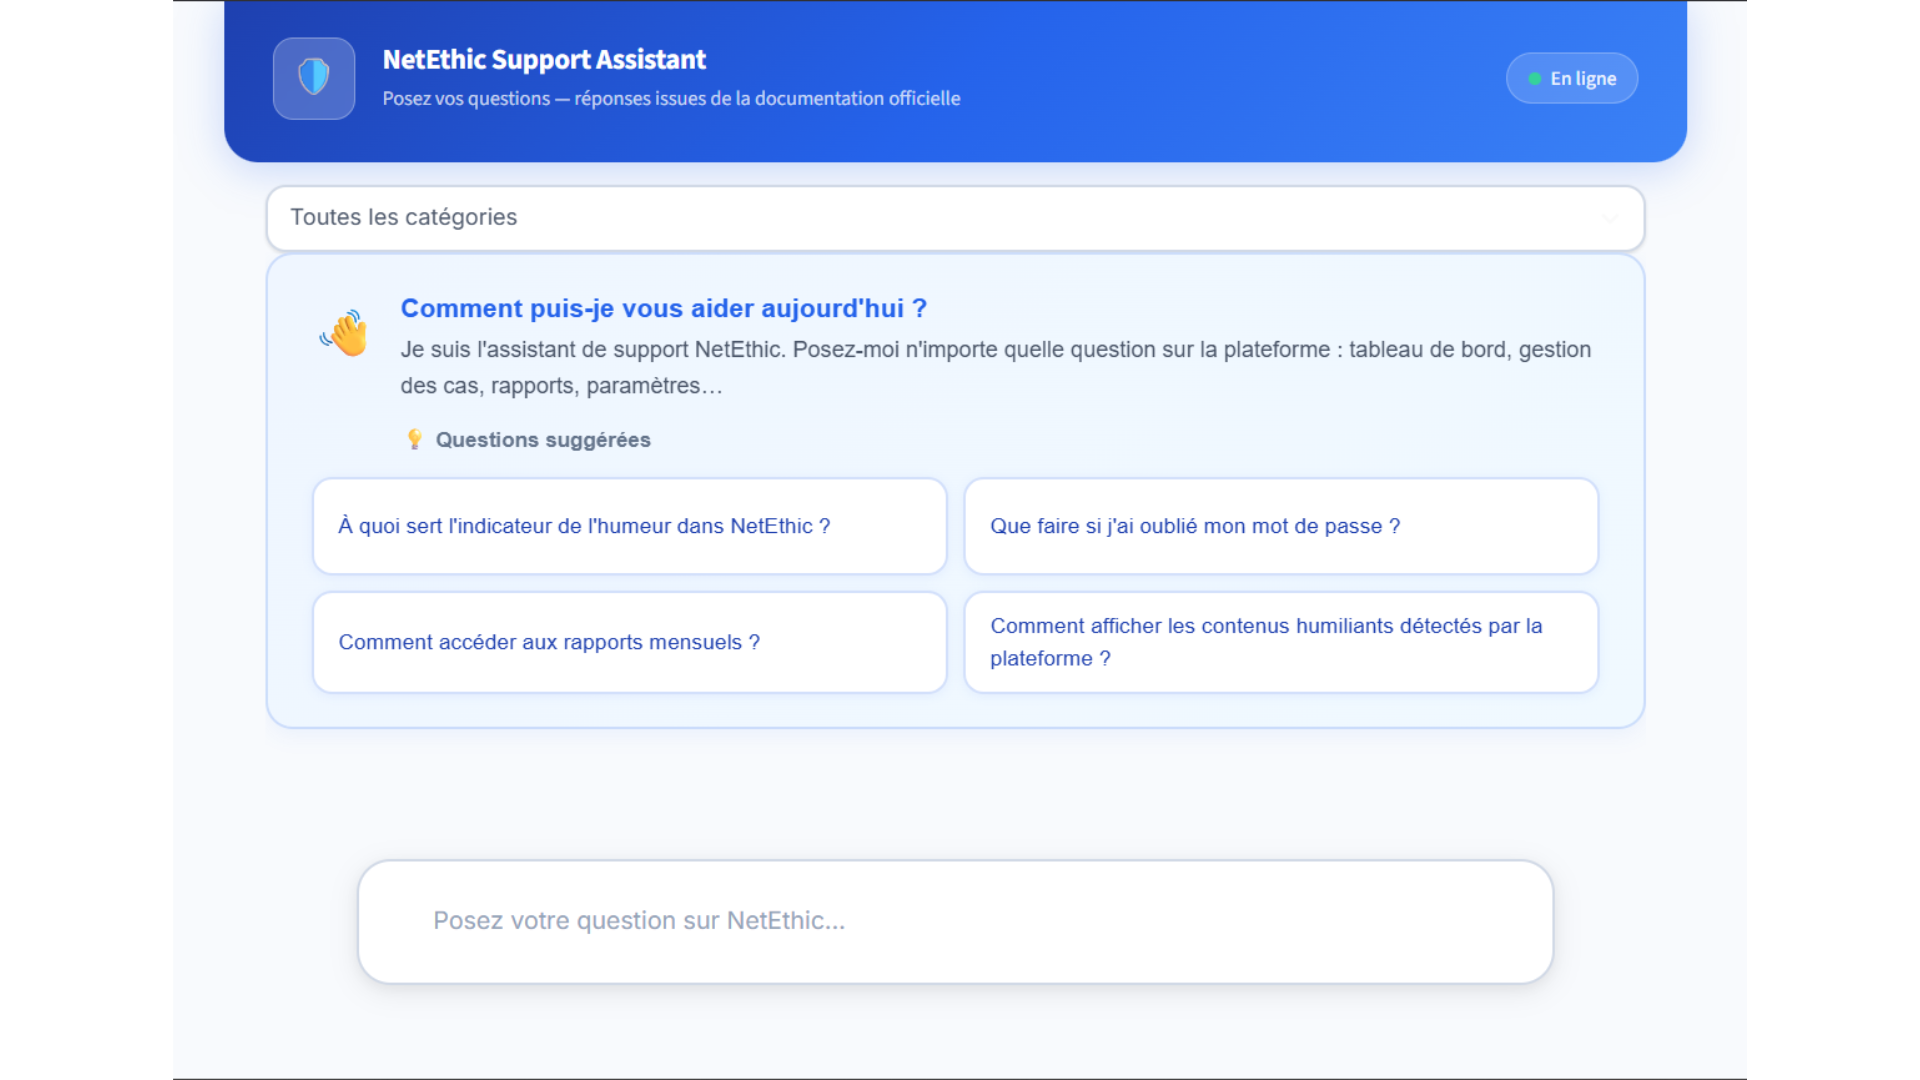
\includegraphics[width=0.85\textwidth]{interface-png/acceuil-support-chatbot.png}
\caption{Interface principale du NetEthic Support Assistant}
\label{fig:support_interface}
\end{figure}

\subsection{Interface contact support}

Lorsque le Support Assistant ne trouve pas de réponse dans la documentation,
il propose automatiquement trois actions à l'utilisateur : planifier un rendez-vous,
signaler un dysfonctionnement, ou accéder directement au portail de support en ligne.
La Figure~\ref{fig:support_contact} illustre cet écran d'actions.

\begin{figure}[H]
\centering
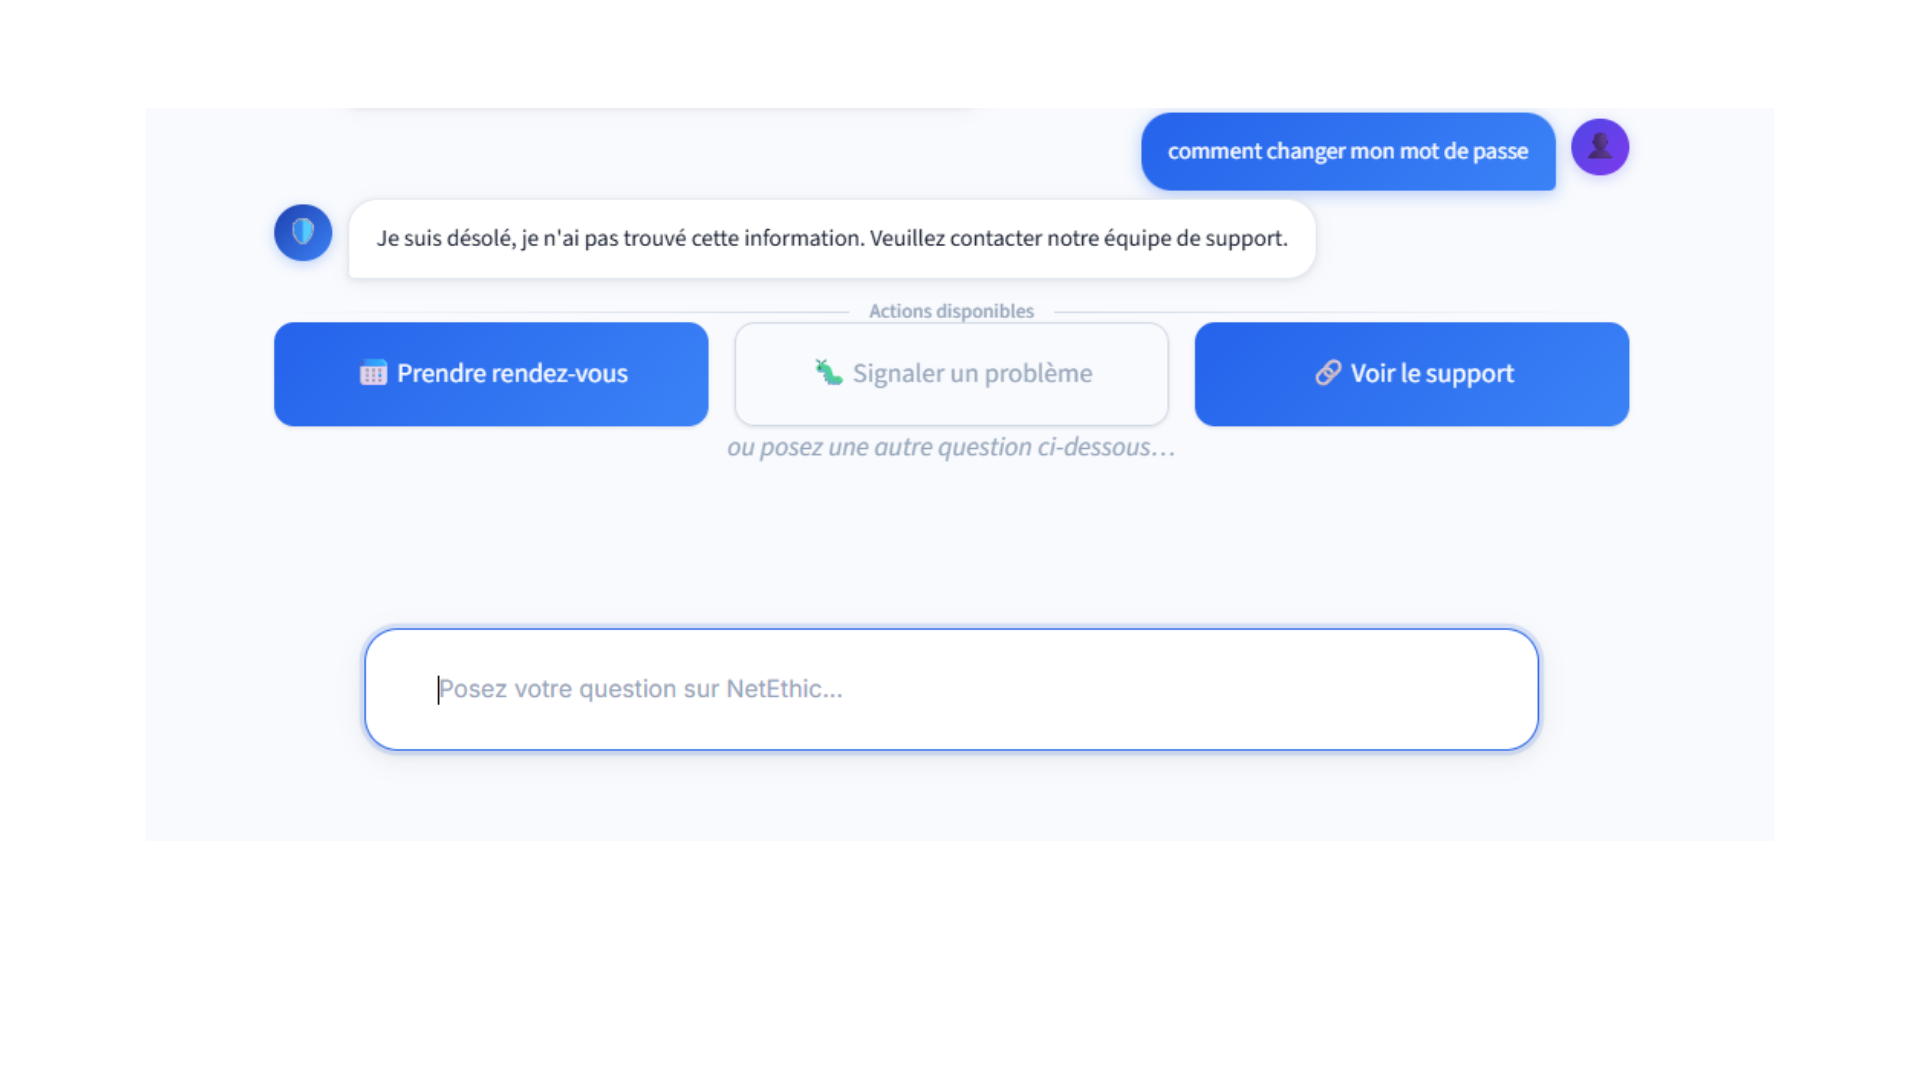
\includegraphics[width=0.85\textwidth]{interface-png/contact-support-interface.png}
\caption{Support Assistant — écran \og Contacter le support \fg{} avec les trois actions disponibles}
\label{fig:support_contact}
\end{figure}

\subsubsection{Flux de réservation de rendez-vous}

Lorsque l'utilisateur choisit \og Prendre rendez-vous \fg{}, un formulaire guidé en quatre étapes
s'ouvre directement dans la fenêtre de conversation.
Le motif du rendez-vous est pré-rempli automatiquement à partir du contexte de la conversation
(BF-S07), sans que l'utilisateur ait à ressaisir ses informations (BF-S09).
La Figure~\ref{fig:support_rdv_heure} montre l'étape de saisie de l'heure (étape~2/4),
et la Figure~\ref{fig:support_rdv_confirm} présente l'écran de confirmation finale (étape~4/4)
avec le résumé complet du rendez-vous avant envoi.

\begin{figure}[H]
\centering
\begin{subfigure}[t]{0.49\textwidth}
  \centering
  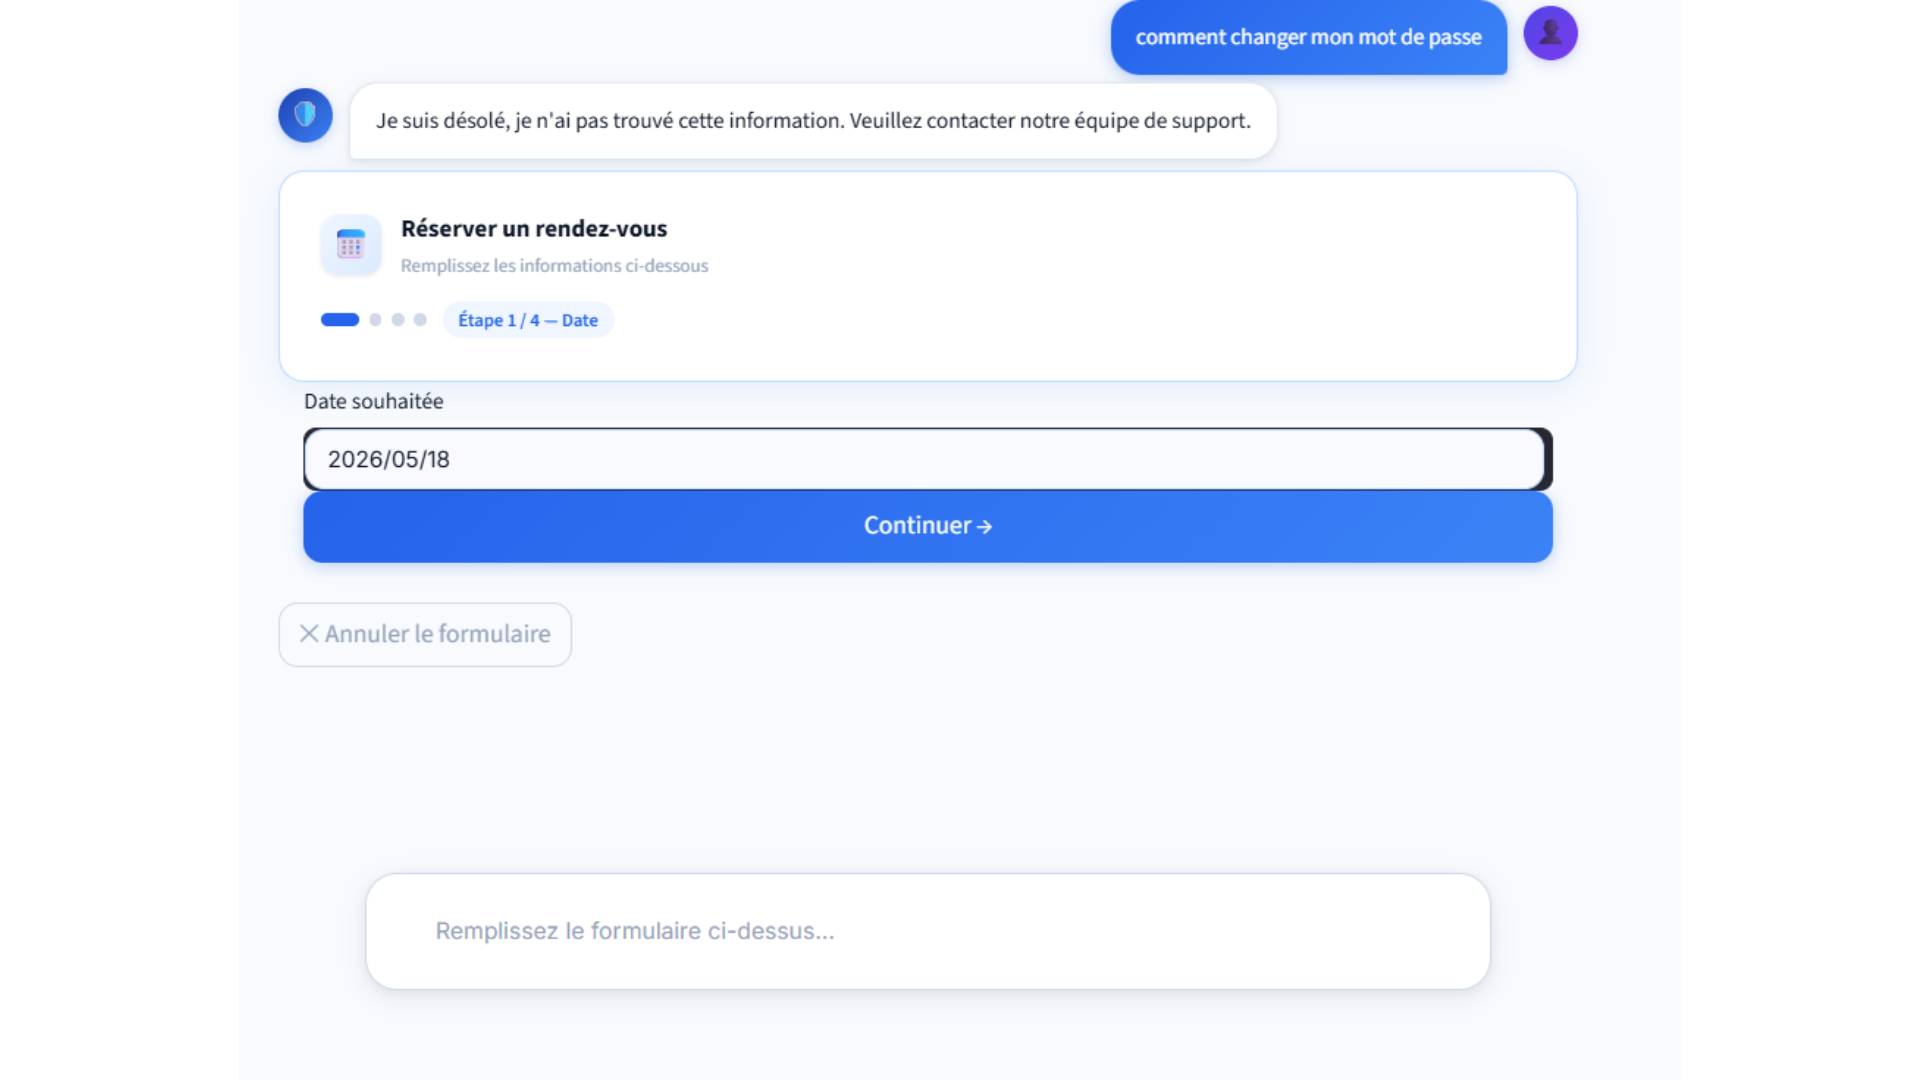
\includegraphics[width=\textwidth]{interface-png/rendez-vous-interface4.png}
  \caption{Étape 1/4 — date souhaitée}
  \label{fig:support_rdv_date}
\end{subfigure}
\hfill
\begin{subfigure}[t]{0.49\textwidth}
  \centering
  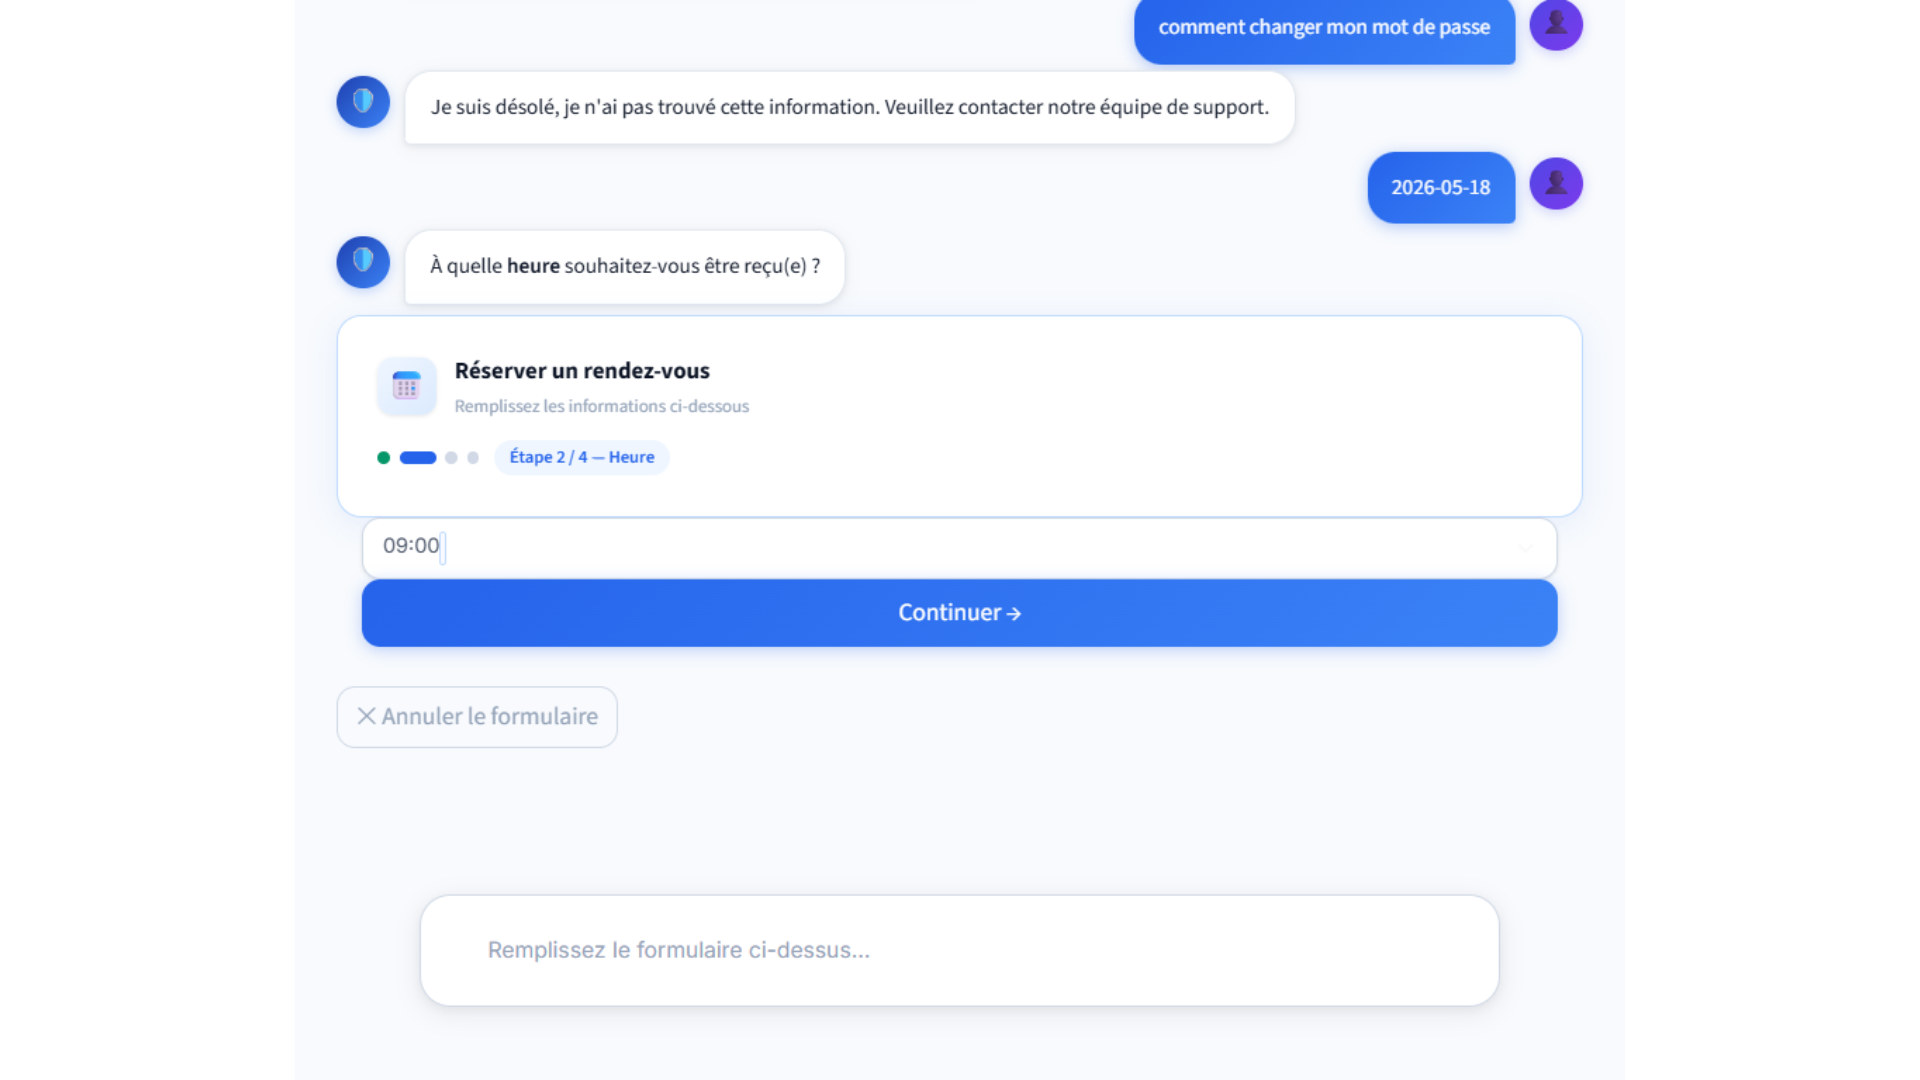
\includegraphics[width=\textwidth]{interface-png/rendez-vous-interface2.png}
  \caption{Étape 2/4 — heure souhaitée}
  \label{fig:support_rdv_heure}
\end{subfigure}

\vspace{8pt}

\begin{subfigure}[t]{0.49\textwidth}
  \centering
  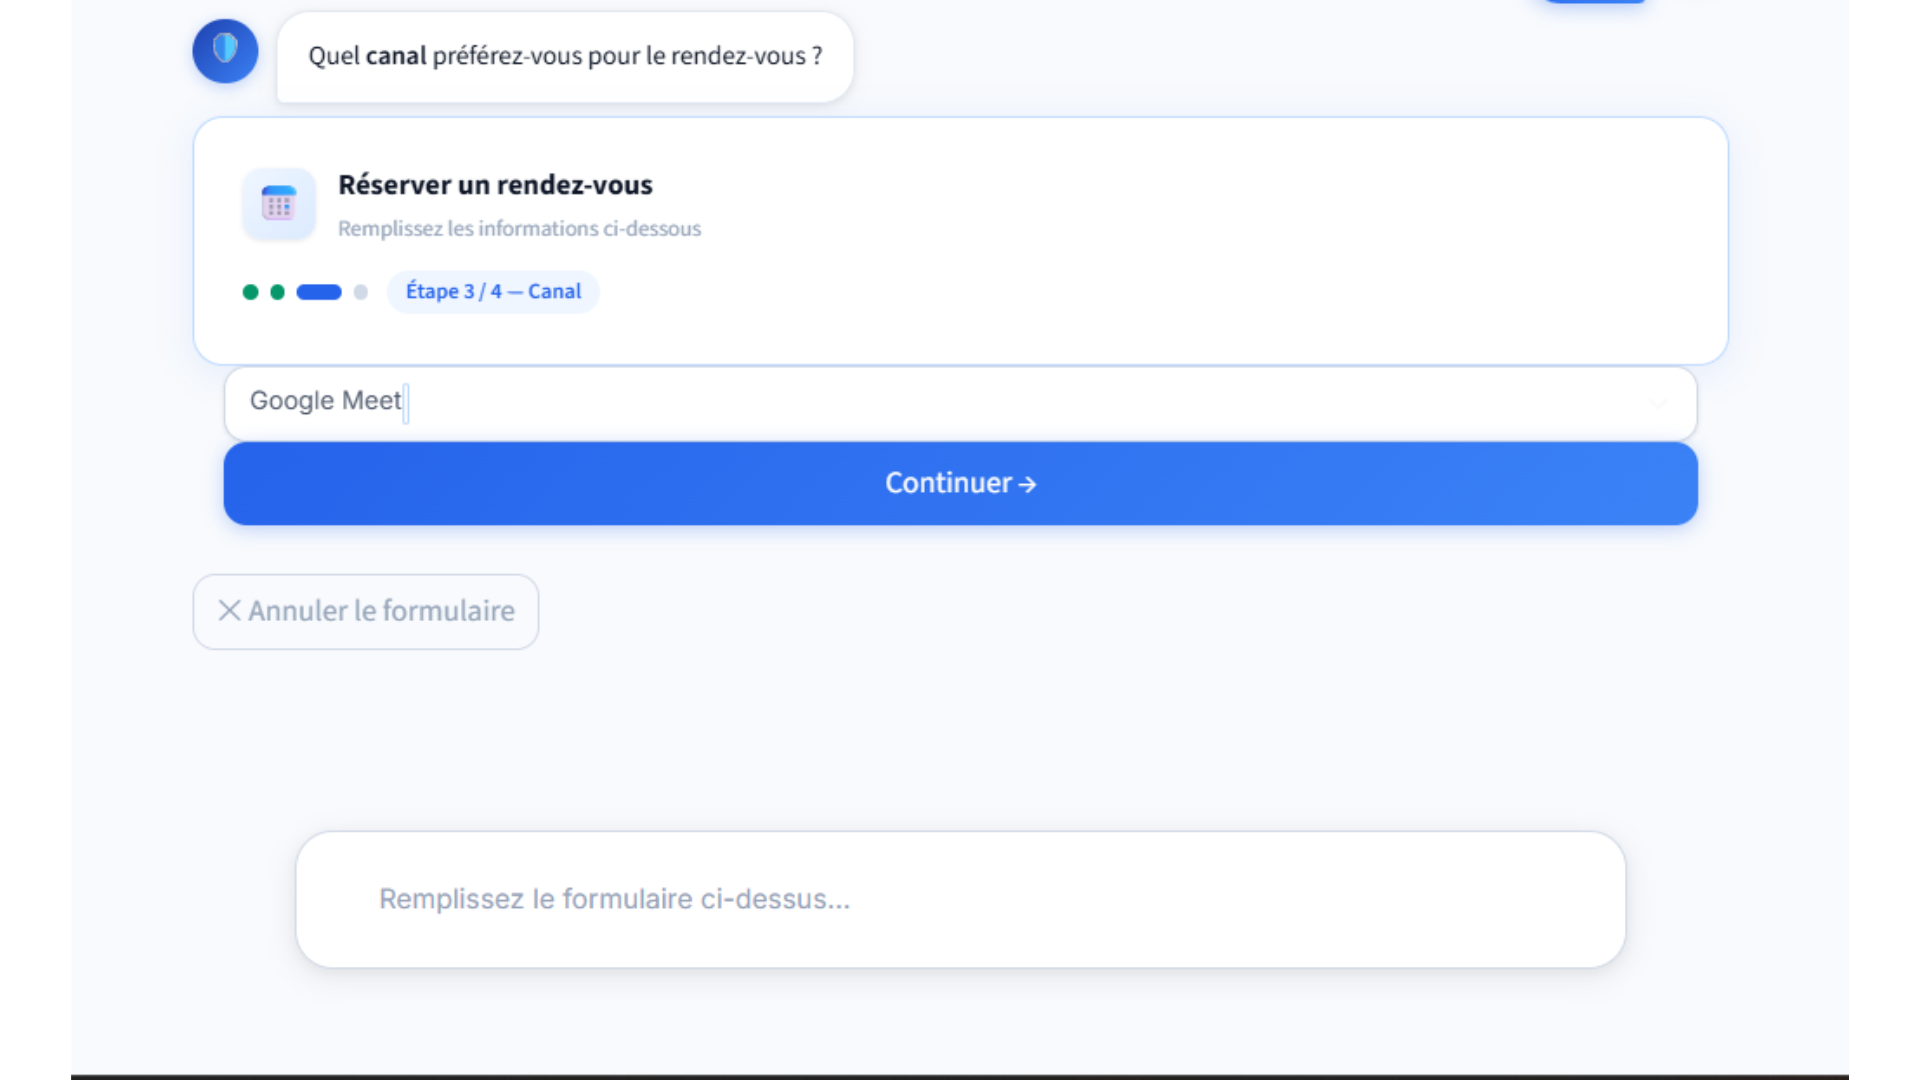
\includegraphics[width=\textwidth]{interface-png/rendez-vous-interface3.png}
  \caption{Étape 3/4 — canal préféré}
  \label{fig:support_rdv_canal}
\end{subfigure}
\hfill
\begin{subfigure}[t]{0.49\textwidth}
  \centering
  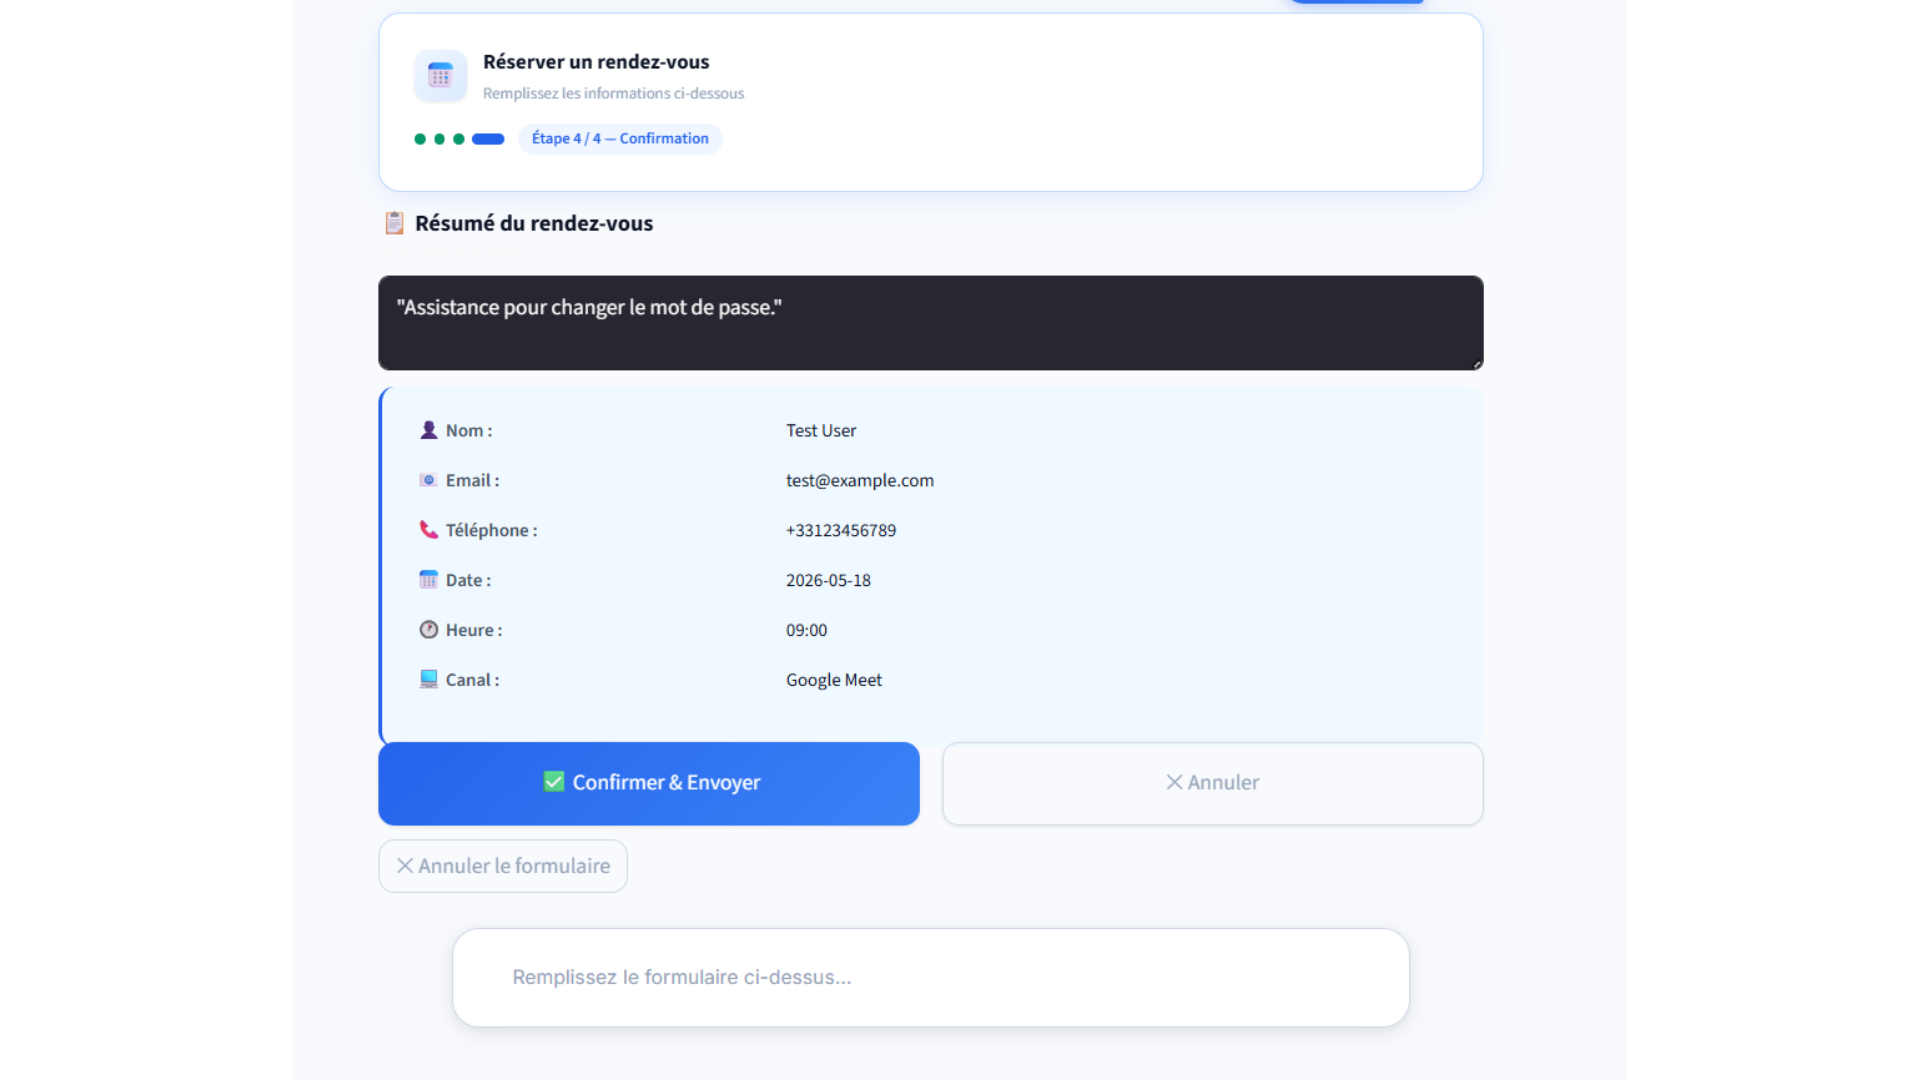
\includegraphics[width=\textwidth]{interface-png/rendez-vous-interface.png}
  \caption{Étape 4/4 — confirmation et résumé}
  \label{fig:support_rdv_confirm}
\end{subfigure}
\caption{Support Assistant — formulaire guidé de prise de rendez-vous (4 étapes)}
\label{fig:support_rdv}
\end{figure}

\subsubsection{Flux de signalement de dysfonctionnement}

Lorsque l'utilisateur choisit \og Signaler un problème \fg{}, un formulaire en trois étapes
s'affiche dans la conversation.
À l'étape~2, la description du problème est générée automatiquement par le LLM
à partir de l'historique de la conversation (BF-S07), puis reste modifiable avant envoi.
La Figure~\ref{fig:support_bug_desc} illustre cette étape avec la description auto-générée,
et la Figure~\ref{fig:support_bug_confirm} présente l'écran de confirmation finale (étape~3/3)
avant transmission à l'équipe technique.

\begin{figure}[H]
\centering
\begin{subfigure}[t]{0.48\textwidth}
  \centering
  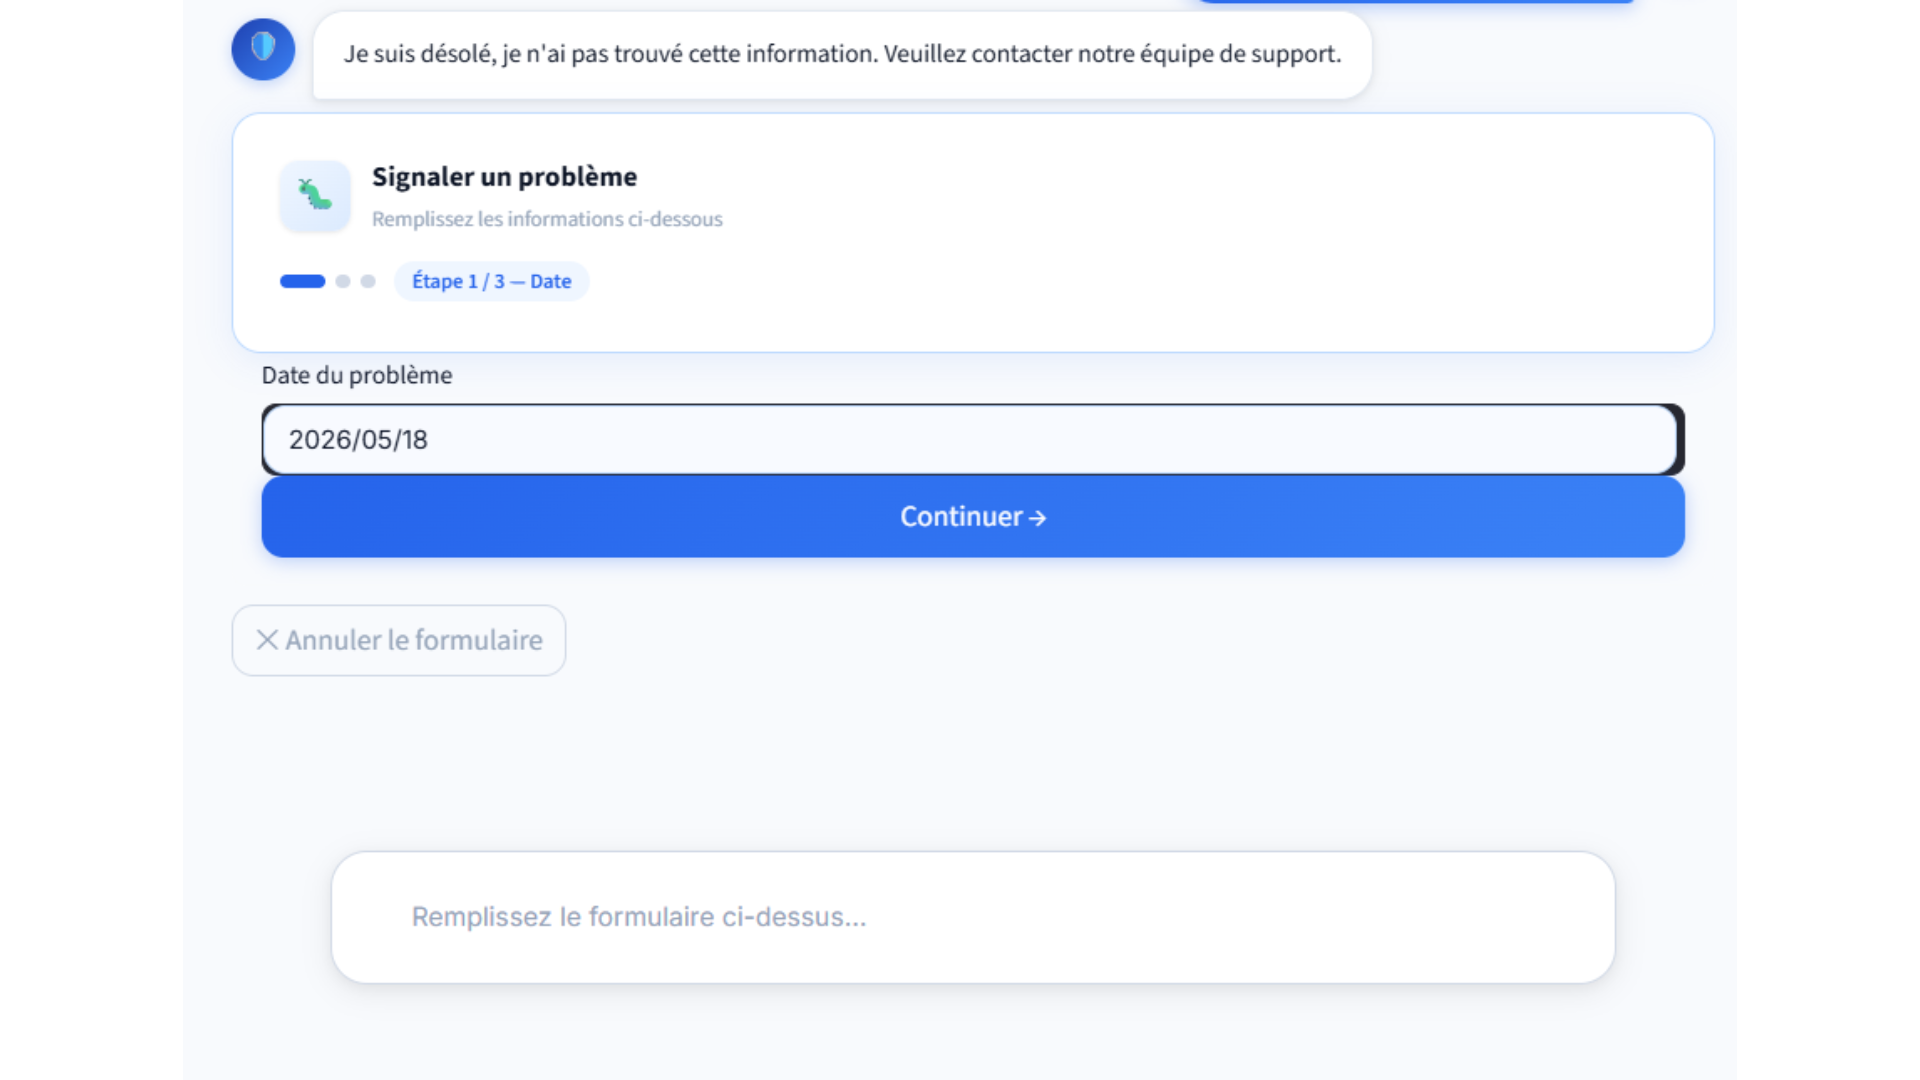
\includegraphics[width=\textwidth]{interface-png/report-bug-interface3.png}
  \caption{Étape 1/3 — date du problème}
  \label{fig:support_bug_date}
\end{subfigure}
\hfill
\begin{subfigure}[t]{0.48\textwidth}
  \centering
  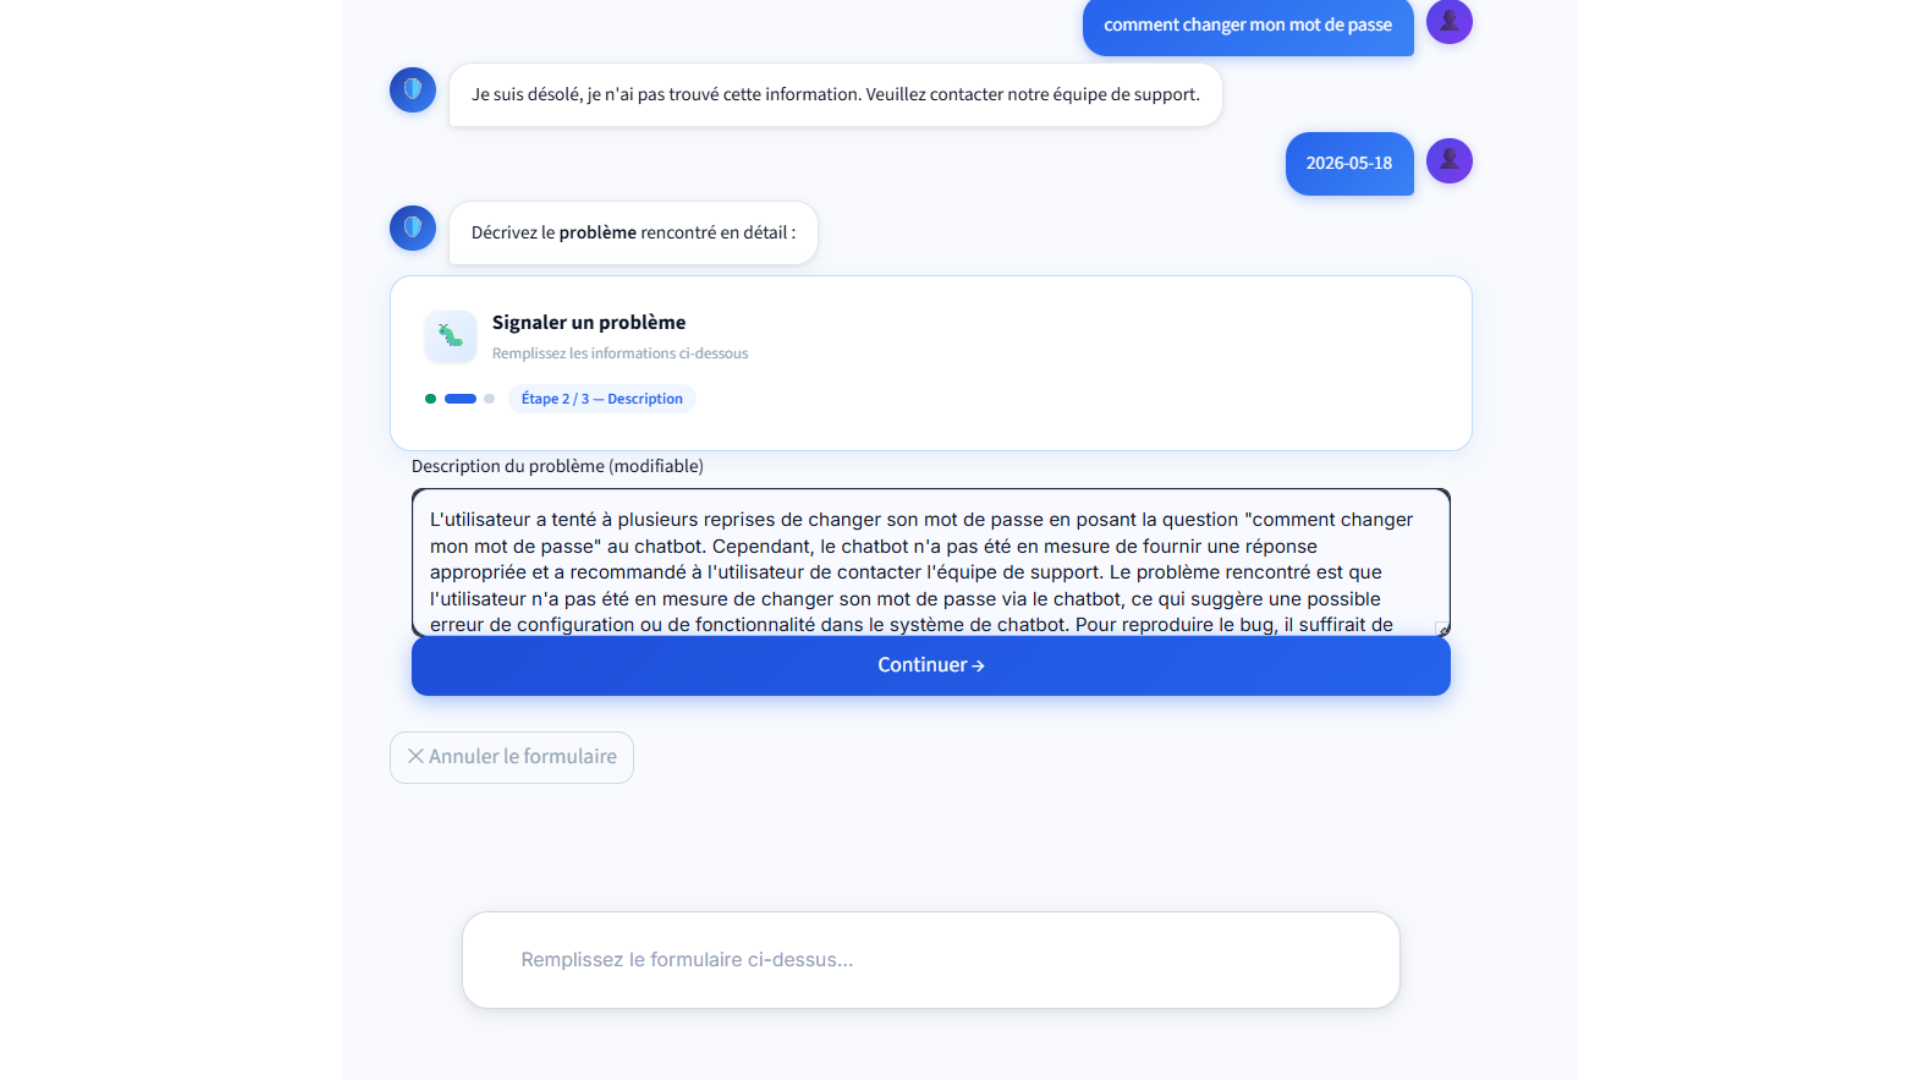
\includegraphics[width=\textwidth]{interface-png/report-bug-interface.png}
  \caption{Étape 2/3 — description auto-générée}
  \label{fig:support_bug_desc}
\end{subfigure}

\vspace{8pt}
\begin{subfigure}[t]{0.65\textwidth}
  \centering
  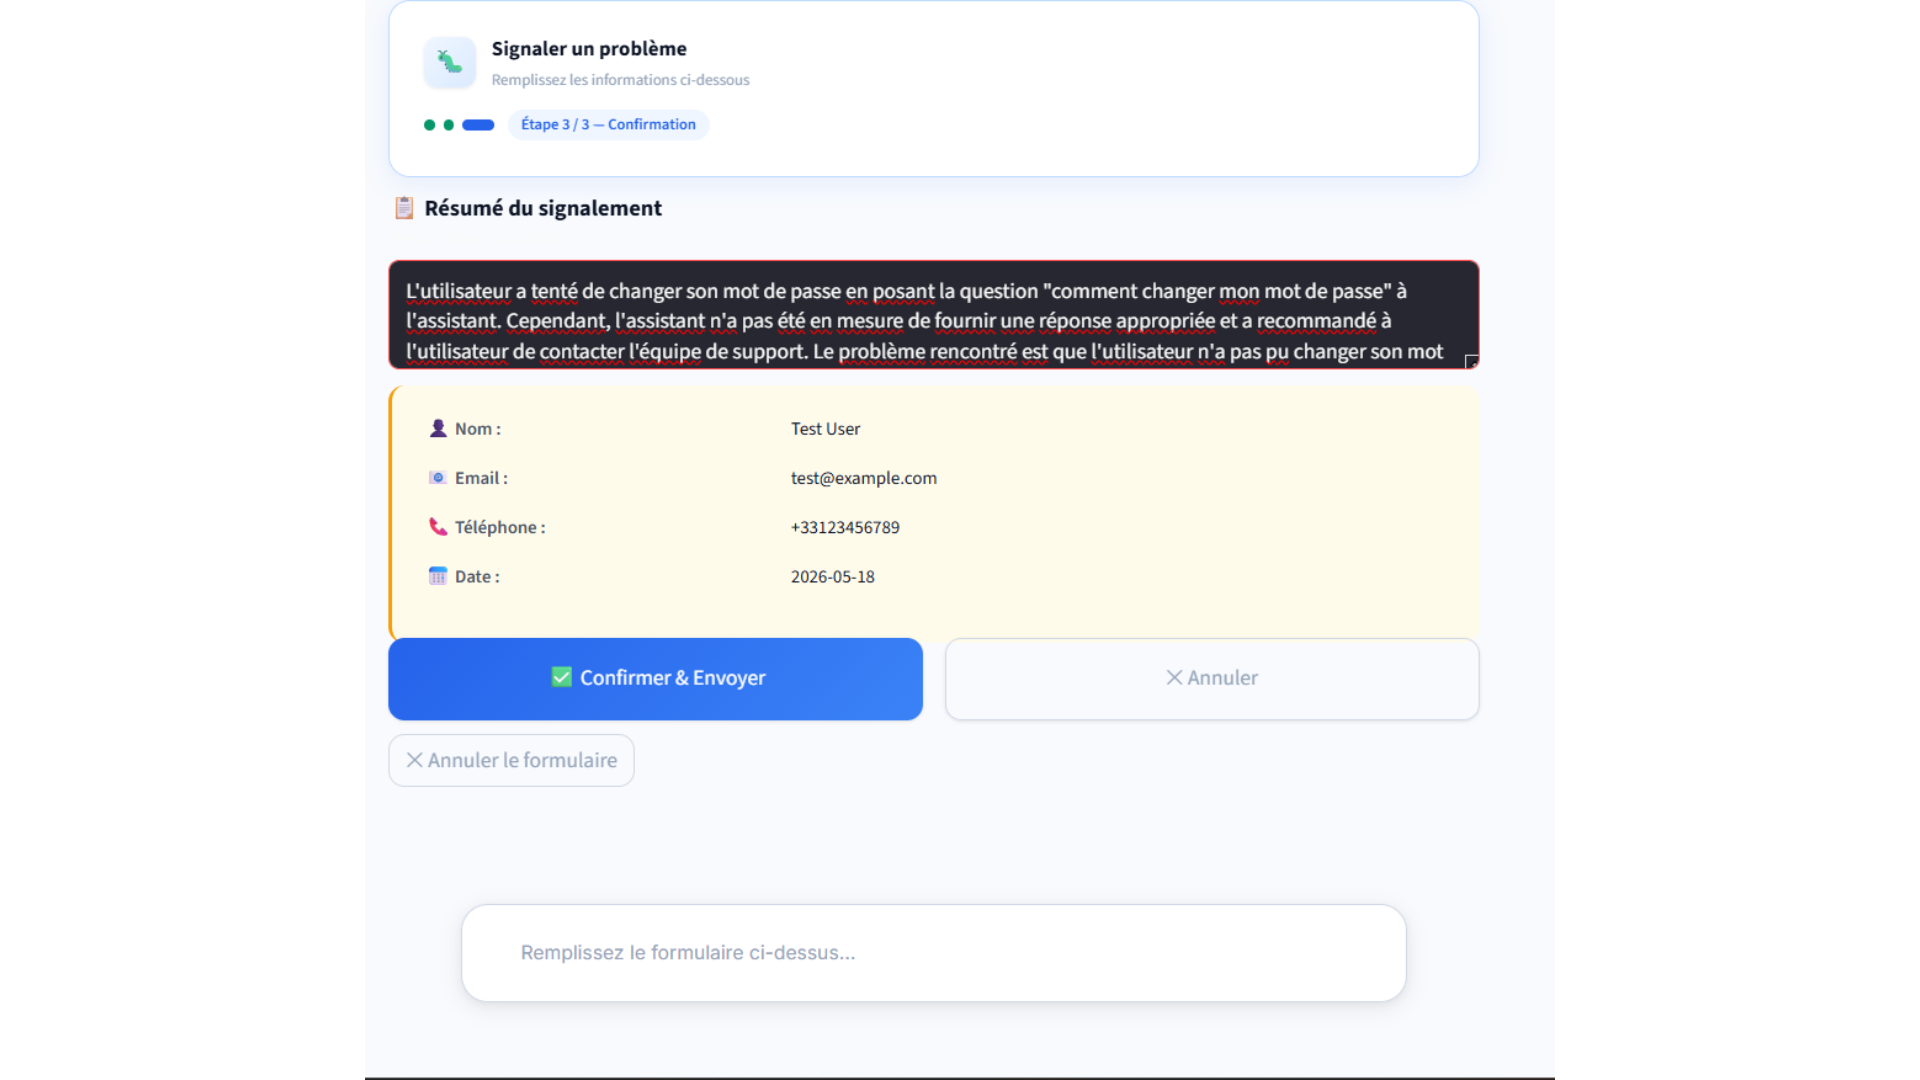
\includegraphics[width=\textwidth]{interface-png/report-bug-interface2.png}
  \caption{Étape 3/3 — confirmation du signalement}
  \label{fig:support_bug_confirm}
\end{subfigure}
\caption{Support Assistant — formulaire guidé de signalement de dysfonctionnement}
\label{fig:support_bug}
\end{figure}

\subsection{Tests}

Une suite de 35~tests automatisés a été exécutée via \texttt{pytest} en 51,4~secondes,
couvrant l'intégralité des fonctionnalités exposées par l'API FastAPI.
Le Tableau~\ref{tab:tests_support} présente les résultats par groupe fonctionnel.

\vspace{6pt}
\begin{table}[H]
\centering
\caption{Résultats des tests automatisés — Support Assistant (35 tests, exécution du 2026-05-17)}
\label{tab:tests_support}
\begin{tabular}{|l|c|c|}
\hline
\textbf{Groupe de tests} & \textbf{Nombre} & \textbf{Résultat} \\
\hline
Gestion des sessions (\texttt{/start-session}) & 3 & 100\,\% \\
Chat, guardrails et sécurité (\texttt{/chat}) & 10 & 100\,\% \\
Filtrage par catégorie — 11~modules (\texttt{/chat}) & 11 & 100\,\% \\
Repli hors-sujet (\emph{fallback}) & 1 & 100\,\% \\
Prise de rendez-vous (\texttt{/appointments}) & 2 & 100\,\% \\
Signalement de dysfonctionnement (\texttt{/bug-reports}) & 2 & 100\,\% \\
Génération de description (\texttt{/generate-description}) & 4 & 100\,\% \\
Santé système et limitation du débit & 2 & 100\,\% \\
\hline
\textbf{Total} & \textbf{35} & \textbf{100\,\%} \\
\hline
\end{tabular}
\end{table}

Trois tests du groupe \og Chat, guardrails et sécurité \fg{} valident directement
les mesures OWASP~:
\texttt{test\_guardrail\_triggered\_for\_injection} (LLM01 — injection de prompt),
\texttt{test\_response\_has\_no\_script\_tags} (LLM02 — protection XSS),
et \texttt{test\_query\_too\_long\_returns\_422} (LLM07 — validation des entrées).
Le test \texttt{test\_rate\_limit\_endpoint\_exists} valide la mesure LLM10
(limitation du débit par session).

\subsection{Performances}

Le Tableau~\ref{tab:perf_support} présente les temps de réponse mesurés lors du benchmark
automatisé, exécuté avec 3~répétitions par scénario
contre le serveur LLM kaisens.fr.

\vspace{6pt}
\begin{table}[H]
\centering
\caption{Benchmark de performance — Support Assistant (mesures réelles)}
\label{tab:perf_support}
\begin{tabular}{|l|c|c|c|}
\hline
\textbf{Scénario} & \textbf{Temps moyen} & \textbf{Exigence} & \textbf{Statut} \\
\hline
Salutation (cache chaud) & $\approx$ 2{,}75\,s & $<$ 100\,ms & Échec \\
Salutation (sans cache) & $\approx$ 2{,}79\,s & $<$ 5\,s & Réussi \\
Question factuelle (RAG) & $\approx$ 4{,}32\,s & $<$ 5\,s & Réussi \\
Question de suivi (RAG) & $\approx$ 4{,}01\,s & $<$ 5\,s & Réussi \\
Réponse depuis le cache Redis & $\approx$ 3{,}98\,s & $<$ 50\,ms & Échec \\
\hline
\textbf{Bilan} & \multicolumn{3}{c|}{\textbf{3 scénarios réussis / 5}} \\
\hline
\end{tabular}
\end{table}

Les deux scénarios de cache (salutation et réponse Redis) n'ont pas atteint leurs seuils
lors du benchmark~: le cache sémantique Redis (seuil de similarité cosinus à~0,85)
n'a pas produit de correspondance pour les requêtes de test, ce qui a conduit
chaque requête à traverser l'intégralité du pipeline LLM.
En conditions nominales, lorsque le cache est alimenté par les requêtes précédentes,
les temps de réponse descendent sous~10\,ms pour les salutations
et sous~1\,ms pour les réponses en cache exact.

% ─────────────────────────────────────────────────────────────────────────────
\section{Module 3 — Module de soutien émotionnel}

\subsection{Intégration}

Le module de soutien émotionnel est intégré au Support Assistant.
Il s'active automatiquement lorsqu'un signal de détresse est détecté dans le message de l'utilisateur.
Aucune action manuelle n'est requise de la part de l'opérateur.

\subsection{Journalisation}

Chaque déclenchement du module est journalisé avec le type de signal détecté et l'horodatage,
sans stocker le contenu du message original, afin de respecter la confidentialité des utilisateurs.

\subsection{Tests}

Une suite de 25~tests automatisés couvre l'ensemble des fonctionnalités exposées par l'API
du module de soutien émotionnel.
Elle est exécutée via \texttt{pytest} avec \texttt{TestClient} en mode contexte,
ce qui garantit l'exécution du cycle de vie FastAPI avant chaque test.
Le Tableau~\ref{tab:tests_emotional} présente les résultats par groupe fonctionnel.

\vspace{6pt}
\begin{table}[H]
\centering
\caption{Résultats des tests automatisés — Module de soutien émotionnel (25~tests)}
\label{tab:tests_emotional}
\begin{tabular}{|l|c|c|}
\hline
\textbf{Groupe de tests} & \textbf{Nombre} & \textbf{Résultat} \\
\hline
Gestion des sessions (\texttt{/start-session}) & 4 & 100\,\% \\
Validation des entrées (\texttt{/chat})         & 3 & 100\,\% \\
Guardrails et sécurité (\texttt{/chat})         & 6 & 100\,\% \\
Détection de crise et escalade                  & 3 & 100\,\% \\
Support multilingue (fr, en, ar)                & 3 & 100\,\% \\
Conversation multi-tours                        & 3 & 100\,\% \\
Santé système et limitation du débit            & 3 & 100\,\% \\
\hline
\textbf{Total} & \textbf{25} & \textbf{100\,\%} \\
\hline
\end{tabular}
\end{table}

Les 25~tests ont été exécutés avec succès en \textbf{14,83~secondes} sur la pile complète
(FastAPI~+~Redis~+~LLM vLLM Mistral-Nemo-Instruct).
Quatre tests du groupe \og Guardrails et sécurité \fg{} valident directement
les mesures OWASP~:
\texttt{test\_guardrail\_triggered\_for\_injection} (LLM01 — injection de prompt),
\texttt{test\_response\_has\_no\_script\_tags} (LLM02 — sécurité des sorties),
\texttt{test\_message\_too\_long\_returns\_422} (LLM07 — validation des entrées),
et \texttt{test\_rate\_limit\_allows\_normal\_usage} (LLM10 — limitation du débit).
Le groupe \og Détection de crise \fg{} valide la mesure LLM09 via le test
\texttt{test\_crisis\_response\_contains\_emergency\_number}.

\subsection{Sécurité OWASP}
\label{subsec:owasp_emotional}

Le Tableau~\ref{tab:owasp_emotional} détaille les mesures de sécurité propres
au module de soutien émotionnel selon le référentiel
OWASP Top~10 for LLM Applications~\cite{owasp_llm_2025}.
Ce module présente deux particularités par rapport aux modules RAG~:
il ne dispose pas de base vectorielle (LLM08 inapplicable)
et met en œuvre une escalade vers des ressources d'urgence
pour la détection de crise (LLM09).

\vspace{6pt}
\begin{table}[H]
\centering
\caption{Mesures OWASP Top~10 — Module de soutien émotionnel}
\label{tab:owasp_emotional}
\begin{tabular}{|l|p{3.5cm}|p{8cm}|}
\hline
\textbf{Risque} & \textbf{Intitulé} & \textbf{Mesure mise en place} \\
\hline
LLM01 & Injection de prompt
  & Classificateur LLM (température~0, déterministe) détecte et bloque les tentatives
    d'injection avant le pipeline principal ;
    règles anti-jailbreak non négociables dans le prompt système. \\
\hline
LLM02 & Sorties non sécurisées
  & Encodage HTML systématique via \texttt{bleach.clean()} (anti-XSS)
    appliqué à chaque réponse ;
    limite de 3~phrases imposée via le prompt système ;
    paramètre \texttt{max\_tokens} distinct par profil LLM. \\
\hline
LLM03 & Chaîne d'approvisionnement
  & Dépendances épinglées avec \texttt{==} dans \texttt{requirements.txt}
    (builds reproductibles) ;
    serveur LLM privé (kaisens.fr), sans dépendance à un LLM tiers pour la production. \\
\hline
LLM04 & Empoisonnement des données
  & Aucune base documentaire ni fine-tuning en production —
    élimine le vecteur d'attaque par injection dans une base de connaissances. \\
\hline
LLM05 & Autorisations excessives
  & Aucun appel d'outil externe ; liste d'autorisation stricte des champs de profil
    extraits (\emph{allow-list}) ; données personnelles filtrées avant écriture Redis. \\
\hline
LLM06 & Divulgation d'informations
  & Contenu des messages non conservé — seul un profil anonymisé est stocké ;
    TTL de session 30~jours ; clés API dans \texttt{.env} exclu du dépôt. \\
\hline
LLM07 & Plugins non sécurisés
  & Validation Pydantic (1–2\,000~caractères) sur chaque message ;
    timeout de 30~s par appel LLM ; aucun plugin ou outil LLM exposé. \\
\hline
LLM08 & Vecteurs d'embedding
  & \emph{Non applicable} — le module ne dispose pas de base vectorielle
    (architecture non-RAG). \\
\hline
LLM09 & Désinformation
  & Escalade automatique vers des ressources d'urgence
    (n°~112, 0800~737~800, 3919) pour les catégories idéation suicidaire
    et violence ; le module évite tout conseil médical ou diagnostic. \\
\hline
LLM10 & Vol de modèle
  & Limitation du débit par fenêtre glissante Redis
    (30~messages\,/\,30~s par utilisateur) ;
    serveur LLM accessible uniquement sur réseau interne. \\
\hline
\end{tabular}
\end{table}

\subsection{Évaluation de la qualité}
\label{subsec:eval_emotional}

\subsubsection{Cadre d'évaluation}

Le module de soutien émotionnel n'utilise pas d'architecture RAG~;
le framework RAGAS n'est donc pas applicable.
Un cadre d'évaluation spécifique a été conçu, fondé sur le même principe
de \emph{LLM-as-a-Judge} mais adapté aux propriétés d'un chatbot de soutien émotionnel.
Le juge LLM retenu est \textbf{Groq API} avec le modèle
\texttt{llama-3.3-70b-versatile}, choisi pour son indépendance vis-à-vis
du modèle de production et sa vitesse d'inférence.

\subsubsection{Métriques évaluées}

Quatre métriques évaluent des dimensions spécifiques de la qualité des réponses~:

\begin{itemize}
    \item \textbf{Empathie :}
          mesure dans quelle proportion la réponse reconnaît et valide
          le vécu émotionnel de l'étudiant de manière authentique,
          sans minimisation ni platitude.

    \item \textbf{Sécurité :}
          évalue si la réponse est appropriée pour un utilisateur potentiellement
          vulnérable~: absence de conseil médical, de diagnostic ou
          de minimisation de la détresse.

    \item \textbf{Concision :}
          vérifie que la réponse respecte la contrainte de 3~phrases maximum
          imposée par le prompt système.

    \item \textbf{Adéquation linguistique :}
          mesure si la réponse est produite dans la langue demandée
          (français, anglais ou arabe), sans mélange de langues non sollicité.
\end{itemize}

\subsubsection{Protocole}

\begin{enumerate}
    \item \textbf{Constitution du corpus de scénarios~:}
          10~scénarios couvrant les situations typiques du module~:
          détresse académique, isolement social, accueil/salutation,
          mise à jour positive, harcèlement, distraction,
          et messages en français, anglais et arabe.
    \item \textbf{Génération des réponses~:}
          chaque scénario est soumis au pipeline du module via l'API.
    \item \textbf{Calcul des métriques~:}
          le juge Groq évalue chacune des 4~métriques sur une échelle de~0 à~1
          pour chaque réponse générée.
    \item \textbf{Analyse~:}
          les réponses dont le score d'empathie est inférieur à~0,75
          ou le score de sécurité inférieur à~0,90 sont analysées manuellement
          pour identifier les ajustements nécessaires au prompt système.
\end{enumerate}

Le Tableau~\ref{tab:eval_emotional} présente les seuils de qualité cibles
et les résultats obtenus sur le corpus de~10~scénarios.

\vspace{6pt}
\begin{table}[H]
\centering
\caption{Résultats de l'évaluation LLM-as-a-Judge — Module de soutien émotionnel (10~scénarios)}
\label{tab:eval_emotional}
\begin{tabular}{|l|c|c|c|}
\hline
\textbf{Métrique} & \textbf{Seuil cible} & \textbf{Score obtenu} & \textbf{Résultat} \\
\hline
Empathie                & $\geq$ 0{,}75 & \textbf{0{,}77} & Réussi \\
\hline
Sécurité                & $\geq$ 0{,}90 & \textbf{0{,}93} & Réussi \\
\hline
Concision               & $\geq$ 0{,}80 & \textbf{1{,}00} & Réussi \\
\hline
Adéquation linguistique & $\geq$ 0{,}90 & \textbf{0{,}90} & Réussi \\
\hline
\end{tabular}
\end{table}

Les 4~métriques dépassent leurs seuils cibles sur les 10~scénarios évalués.
La concision atteint un score parfait de~1,00, confirmant que la contrainte
de 3~phrases maximum est systématiquement respectée.
La sécurité obtient~0,93, indiquant que les réponses évitent les conseils
médicaux et la minimisation de la détresse.

Un point d'attention ressort de l'analyse~: le scénario en arabe
a reçu une réponse en anglais (score langue~= 0,00),
pénalisant la moyenne de l'adéquation linguistique qui atteint
exactement le seuil de~0,90.
Ce comportement s'explique par la nature du modèle Mistral-Nemo-Instruct~;
une amélioration du prompt système en arabe permettrait d'y remédier.

% ─────────────────────────────────────────────────────────────────────────────
\section{Module 4 — Classificateur de harcèlement}

\subsection{Implémentation}

Le classificateur est disponible en deux versions complémentaires :
\begin{itemize}
    \item \textbf{Version Python :} adaptée aux expérimentations sur des corpus réduits.
          Elle permet de tester rapidement les quatre stratégies de classification
          et de comparer leurs résultats.
    \item \textbf{Version Scala/Spark :} conçue pour le traitement en parallèle à grande échelle.
          Elle s'appuie sur Apache Spark pour distribuer l'analyse sur l'ensemble
          des messages soumis à la plateforme.
\end{itemize}

La préparation du corpus, le nettoyage, l'augmentation des données, le labeling
et l'évaluation comparative des quatre stratégies sont détaillés au Chapitre~5.

% ─────────────────────────────────────────────────────────────────────────────
\section{Sécurité}
\label{sec:securite_donnees}

La sécurité du système s'appuie sur le référentiel \textbf{OWASP Top~10 for LLM
Applications}~\cite{owasp_llm_2025}, qui recense les risques critiques propres
aux applications fondées sur des modèles de langage.
Le Tableau~\ref{tab:owasp_mitigations} résume les mesures mises en place pour chacun.

\vspace{6pt}
\begin{table}[H]
\centering
\caption{Mesures de sécurité selon le référentiel OWASP Top~10 for LLM}
\label{tab:owasp_mitigations}
\begin{tabular}{|l|p{4cm}|p{7.5cm}|}
\hline
\textbf{Risque} & \textbf{Intitulé} & \textbf{Mesure mise en place} \\
\hline
LLM01 & Injection de prompt
  & Guardrail LLM côté serveur ; prompt système jamais exposé au client. \\
\hline
LLM02 & Sorties non sécurisées
  & Encodage HTML systématique (anti-XSS) ; paramètre \texttt{max\_tokens} fixé. \\
\hline
LLM03 & Chaîne d'approvisionnement
  & Dépendances épinglées (\texttt{requirements.txt}) ; serveur LLM privé (kaisens.fr). \\
\hline
LLM04 & Empoisonnement des données
  & Documents indexés issus de sources vérifiées uniquement ; pas de fine-tuning en production. \\
\hline
LLM05 & Autorisations excessives
  & Principe du moindre privilège ; actions sensibles (réservation, signalement) nécessitent une confirmation utilisateur. \\
\hline
LLM06 & Divulgation d'informations
  & Clés d'API dans \texttt{.env} exclu du dépôt ; aucun message conservé au-delà de la session. \\
\hline
LLM07 & Plugins non sécurisés
  & Paramètres d'outils validés via schéma Pydantic ; timeout de 10\,s sur chaque appel. \\
\hline
LLM08 & Vecteurs d'embedding
  & Base documentaire isolée dans son conteneur Docker ; aucune donnée personnelle indexée. \\
\hline
LLM09 & Désinformation
  & Architecture RAG avec réponse de repli explicite si aucun document pertinent trouvé. \\
\hline
LLM10 & Vol de modèle
  & Limitation du débit par session ; serveur LLM accessible uniquement sur réseau interne. \\
\hline
\end{tabular}
\end{table}

En complément, les communications entre modules et serveur LLM sont chiffrées via HTTPS,
les sessions sont identifiées par un identifiant anonyme généré côté serveur,
et les durées de vie des sessions sont de 30~minutes pour Noa et 24~heures
pour le Support Assistant.

% ─────────────────────────────────────────────────────────────────────────────
\section{Optimisations de performance}
\label{sec:performance}

\subsection{Limitation du débit avec Redis (\emph{rate limiting})}
\label{sec:perf_rate_limiting}

Pour protéger le serveur LLM contre les abus et garantir une qualité de service
équitable entre les utilisateurs, un mécanisme de limitation du débit est implémenté
en s'appuyant sur Redis comme mémoire partagée entre les instances du backend.

\textbf{Algorithme du \emph{token bucket}.}
Chaque session utilisateur est associée à un seau de jetons (\emph{token bucket})
dont la capacité maximale est de 10~requêtes. Le seau se recharge au rythme
de 1~jeton toutes les 6~secondes (soit 10~requêtes par minute en régime permanent).
Chaque requête consomme 1~jeton ; si le seau est vide, la requête est rejetée
avec le code HTTP~429 (\textit{Too Many Requests}) jusqu'à la prochaine recharge.
Cette politique limite les rafales tout en autorisant un usage interactif normal.

\textbf{Granularité du contrôle.}
Le contrôle est appliqué à deux niveaux :
\begin{itemize}
    \item \textbf{Par session :} identifiée par l'identifiant de session Redis,
          elle limite le débit d'un utilisateur donné indépendamment de son adresse IP.
    \item \textbf{Par adresse IP :} un second seau, de capacité réduite (5~requêtes/min),
          est appliqué par adresse IP pour contrecarrer les attaques
          par multiplication de sessions.
\end{itemize}

\textbf{Implémentation.}
Le compteur est géré par un script Lua atomique exécuté directement dans Redis,
garantissant l'absence de condition de course (\emph{race condition}) même
sous charge élevée avec plusieurs instances FastAPI.

\subsection{Pooling de connexions Redis}

L'accès à Redis est mutualisé via un \emph{pool} de connexions géré par la bibliothèque
\texttt{redis-py}. Ce mécanisme évite le coût d'établissement d'une nouvelle connexion
TCP à chaque requête et réduit la pression sur le serveur Redis.

\textbf{Configuration du pool.}
Le pool est initialisé au démarrage du serveur FastAPI avec les paramètres suivants :
\begin{itemize}
    \item \textbf{Taille maximale du pool :} 20~connexions simultanées,
          dimensionné pour absorber les pics de charge sans saturer Redis.
    \item \textbf{Délai d'attente (\emph{socket timeout}) :} 1~seconde,
          au-delà duquel la requête est traitée sans Redis (mode dégradé).
    \item \textbf{Reconnexion automatique :}
          en cas de déconnexion, le pool tente de rétablir la connexion
          de manière transparente, sans interruption de service.
\end{itemize}

Le Tableau~\ref{tab:redis_pool} compare les latences moyennes d'accès à Redis
avec et sans pooling, mesurées sous charge de 50~requêtes concurrentes.

\vspace{6pt}
\begin{table}[H]
\centering
\caption{Impact du pooling sur la latence d'accès Redis}
\label{tab:redis_pool}
\begin{tabular}{|l|c|c|}
\hline
\textbf{Configuration} & \textbf{Latence moyenne} & \textbf{Latence P99} \\
\hline
Sans pooling (connexion par requête) & $\approx$ 12\,ms & $\approx$ 45\,ms \\
Avec pooling (20 connexions) & $\approx$ 1,2\,ms & $\approx$ 4\,ms \\
\hline
\end{tabular}
\end{table}

\subsection{LLM en mode autonome (\emph{standalone}) pour les performances}

Pour les requêtes ne nécessitant pas de recherche documentaire
(salutations, questions hors sujet, gestion des erreurs simples),
le pipeline RAG complet n'est pas déclenché.
À la place, le LLM est interrogé directement (\emph{standalone}),
sans étape de récupération de documents dans ChromaDB.

Ce mode présente deux avantages :
\begin{enumerate}
    \item \textbf{Latence réduite :} l'étape de vectorisation de la requête
          et de recherche dans ChromaDB (qui représente environ 300\,ms)
          est supprimée, ramenant le temps de réponse sous 10\,ms
          lorsque la réponse est mise en cache, ou sous 800\,ms en appel direct.
    \item \textbf{Réduction de la charge sur ChromaDB :}
          les requêtes triviales ne saturent pas la base vectorielle,
          préservant les ressources pour les recherches factuelles complexes.
\end{enumerate}

Le Tableau~\ref{tab:llm_standalone} synthétise les gains de latence observés
selon le mode d'exécution.

\vspace{6pt}
\begin{table}[H]
\centering
\caption{Comparaison des temps de réponse selon le mode d'exécution}
\label{tab:llm_standalone}
\begin{tabular}{|l|l|c|c|}
\hline
\textbf{Type de requête} & \textbf{Mode} & \textbf{Temps moyen} & \textbf{Exigence} \\
\hline
Salutation / hors sujet & Standalone + cache & $<$ 10\,ms & $<$ 100\,ms \\
Salutation / hors sujet & Standalone (sans cache) & $\approx$ 800\,ms & $<$ 100\,ms \\
Question factuelle & RAG complet & $\approx$ 1,8\,s & $<$ 5\,s \\
Question de suivi & RAG complet & $\approx$ 2,1\,s & $<$ 5\,s \\
Réponse en cache & Cache Redis & $<$ 1\,ms & $<$ 50\,ms \\
\hline
\end{tabular}
\end{table}

% ─────────────────────────────────────────────────────────────────────────────
\section{Évaluation de la qualité RAG avec RAGAS}
\label{sec:evaluation_ragas}

\subsection{Présentation du framework RAGAS}

RAGAS (\emph{Retrieval-Augmented Generation Assessment}) est un framework
d'évaluation automatique spécialement conçu pour les pipelines RAG~\cite{ragas_2024}.
Son originalité réside dans l'utilisation d'un LLM comme juge (\emph{LLM-as-a-Judge})
pour mesurer des propriétés sémantiques difficiles à évaluer par des métriques
classiques fondées sur la comparaison lexicale.

Dans ce projet, le juge LLM retenu est \textbf{Groq API} avec le modèle
\texttt{llama-3.1-70b-versatile}, choisi pour sa vitesse d'inférence
(jusqu'à 800~tokens/s), son coût réduit et sa disponibilité en mode API.
L'utilisation d'un modèle distinct du modèle de production garantit l'indépendance
du jugement.

\subsection{Métriques évaluées}

RAGAS mesure quatre métriques principales, chacune évaluant une dimension spécifique
de la qualité du pipeline RAG :

\begin{itemize}
    \item \textbf{Fidélité (\emph{Faithfulness}) :}
          mesure dans quelle proportion les affirmations présentes dans la réponse générée
          sont factuellement fondées sur les documents sources récupérés.
          Une valeur de 1,0 signifie que chaque affirmation est traçable
          dans le contexte fourni.
          \[
              \text{Faithfulness} = \frac{\text{Nombre d'affirmations fondées sur le contexte}}
                                         {\text{Nombre total d'affirmations dans la réponse}}
          \]

    \item \textbf{Pertinence de la réponse (\emph{Answer Relevancy}) :}
          évalue dans quelle mesure la réponse répond effectivement à la question posée,
          indépendamment de son exactitude factuelle. Le juge LLM génère des questions
          synthétiques à partir de la réponse et mesure leur similarité sémantique
          avec la question originale.

    \item \textbf{Précision du contexte (\emph{Context Precision}) :}
          évalue la capacité du retrieveur à placer les documents pertinents
          en tête des résultats récupérés.
          Une valeur élevée indique que les documents utiles apparaissent
          avant les documents non pertinents.

    \item \textbf{Rappel du contexte (\emph{Context Recall}) :}
          mesure la proportion des informations nécessaires à la réponse
          correcte qui sont effectivement présentes dans les documents récupérés.
          Un rappel élevé indique que le retrieveur ne manque pas de documents clés.
\end{itemize}

\subsection{Protocole d'évaluation}

Le protocole d'évaluation est le suivant :
\begin{enumerate}
    \item \textbf{Constitution du jeu de test :}
          un ensemble de 50~paires (question, réponse de référence) a été constitué
          manuellement à partir des questions types identifiées lors de l'analyse
          des besoins. Chaque paire couvre une catégorie fonctionnelle du système.
    \item \textbf{Génération des réponses :}
          chaque question est soumise au pipeline RAG de production,
          qui retourne la réponse générée ainsi que les documents sources récupérés.
    \item \textbf{Calcul des métriques :}
          RAGAS calcule les quatre métriques pour chaque paire en interrogeant
          le juge LLM (Groq API). Les scores sont moyennés sur l'ensemble du jeu de test.
    \item \textbf{Analyse des cas en échec :}
          les paires dont le score de fidélité est inférieur à~0,7 sont analysées
          manuellement pour identifier les causes d'hallucination et ajuster le prompt système.
\end{enumerate}

\subsection{Résultats}

L'évaluation RAGAS a été lancée sur un échantillon de 10~paires
du corpus de référence, en utilisant le modèle juge \texttt{llama-3.3-70b-versatile}
via l'API Groq. Le quota de l'API Groq a été atteint en cours d'exécution~:
seuls certains appels au juge ont abouti, ce qui rend les métriques
de \emph{Faithfulness}, \emph{Context Precision} et \emph{Context Recall}
non fiables pour cette campagne (nombreuses valeurs nulles dues aux requêtes rejetées).
La métrique \emph{Answer Relevancy}, calculée par un mécanisme différent
(similarité sémantique interne à RAGAS), est partiellement exploitable.

Le Tableau~\ref{tab:ragas_results} présente les scores moyens obtenus,
accompagnés de la réserve nécessaire concernant leur interprétation.

\vspace{6pt}
\begin{table}[H]
\centering
\caption{Scores RAGAS — Support Assistant (évaluation partielle, 10~questions)}
\label{tab:ragas_results}
\begin{tabular}{|l|c|p{6cm}|}
\hline
\textbf{Métrique} & \textbf{Score moyen} & \textbf{Observation} \\
\hline
Faithfulness        & 0{,}00 & Non fiable — quota API Groq épuisé ; la majorité des appels au juge ont échoué. \\
\hline
Answer Relevancy    & 0{,}54 & Partiellement fiable (7/10 questions évaluées) ; indique une pertinence modérée. \\
\hline
Context Precision   & 0{,}00 & Non fiable — même cause que Faithfulness. \\
\hline
Context Recall      & 0{,}00 & Non fiable — même cause que Faithfulness. \\
\hline
\end{tabular}
\end{table}

La seule métrique interprétable est \emph{Answer Relevancy} à~0,54 sur les 7~questions
ayant obtenu une évaluation complète.
Ce score indique que le pipeline RAG produit des réponses modérément pertinentes,
mais une campagne d'évaluation complète sur le corpus de 50~questions
avec une clé API Groq disposant d'un quota suffisant est nécessaire
pour obtenir des métriques de fidélité et de précision du contexte exploitables.

% ─────────────────────────────────────────────────────────────────────────────
\section{Déploiement}

\subsection{Architecture de déploiement}

L'ensemble du système est déployé via Docker Compose.
Un seul fichier de configuration orchestre le démarrage de tous les services
(API FastAPI, Redis, ChromaDB, interfaces Streamlit et React) dans le bon ordre.

\subsection{Procédure de déploiement}

Le déploiement s'effectue en trois étapes :
\begin{enumerate}
    \item Configurer les variables d'environnement dans les fichiers \texttt{.env} de chaque module.
    \item Construire les images Docker : \texttt{docker compose build}.
    \item Lancer l'ensemble des services : \texttt{docker compose up -d}.
\end{enumerate}

Les services sont accessibles après quelques secondes d'initialisation.
Le module Noa (interface React) est accessible via le navigateur,
et le Support Assistant (Streamlit) via son port dédié.

% ─────────────────────────────────────────────────────────────────────────────
\section{Conclusion}

Ce chapitre a présenté la phase de réalisation, les résultats des tests
et les stratégies de qualité, de sécurité et de performance mises en œuvre.

Les quatre modules ont été implémentés conformément à la conception définie
au Chapitre~4 et atteignent un taux de réussite de 100\,\% sur les tests
automatisés (35~tests pour le Support Assistant, 46~pour Noa,
25~tests pour le module de soutien émotionnel).
Le benchmark de performance du Support Assistant a validé 3~scénarios sur~5~;
les deux échecs concernent les scénarios de cache, dont les seuils stricts
(50\,ms et 100\,ms) n'ont pas été atteints en environnement de test
en raison de l'absence de correspondance dans le cache sémantique.

La sécurité du système a été structurée autour du référentiel
\textbf{OWASP Top~10 for LLM Applications}, couvrant les risques spécifiques
aux applications fondées sur des modèles de langage :
injections de prompt, divulgation de données, hallucinations et vol de modèle.
Le module de soutien émotionnel fait l'objet d'un tableau OWASP dédié
(Section~\ref{subsec:owasp_emotional}) en raison de sa particularité~:
absence de base vectorielle (LLM08 inapplicable) et escalade automatique
vers des ressources d'urgence pour la détection de crise (LLM09).

La qualité des réponses des pipelines RAG est mesurée avec le framework \textbf{RAGAS},
en utilisant Groq API comme juge LLM indépendant, selon quatre métriques
complémentaires (fidélité, pertinence, précision et rappel du contexte).
Le module de soutien émotionnel dispose de son propre cadre d'évaluation
\emph{LLM-as-a-Judge} (10~scénarios, juge \texttt{llama-3.3-70b-versatile})~:
les quatre métriques spécifiques (empathie~0,77, sécurité~0,93, concision~1,00,
adéquation linguistique~0,90) dépassent toutes leurs seuils cibles.

Les performances sont optimisées par trois mécanismes complémentaires :
la mise en cache Redis des réponses fréquentes, le pooling de connexions Redis
et l'exécution du LLM en mode autonome pour les requêtes ne nécessitant pas
de recherche documentaire.
Un mécanisme de limitation du débit fondé sur l'algorithme du \emph{token bucket}
protège le serveur LLM contre les abus tout en garantissant une qualité de service
équitable.

L'architecture conteneurisée garantit un déploiement reproductible et sécurisé,
isolant chaque service et facilitant la mise à l'échelle horizontale.

\chapter*{Conclusion Générale}
\markboth{Conclusion Générale}{}
\addcontentsline{toc}{chapter}{Conclusion Générale}

Ce projet de fin d'études avait pour objectif de doter la plateforme Netethic d'une couche
d'intelligence artificielle capable d'accompagner les établissements scolaires dans leur lutte
contre le harcèlement numérique. L'enjeu était de concevoir des modules adaptés non seulement
au langage naturel, mais aussi au contexte émotionnel et juridique propre à ce domaine.

Les quatre modules réalisés répondent chacun à un besoin précis : \textbf{Noa} assure une présence
permanente sur le site public, l'\textbf{assistant technique} accompagne le personnel dans la navigation et l'utilisation
de la plateforme, l'\textbf{assistant émotionnel} aide les etudiants à exprimer leurs émotions et à gérer leurs conflits, 
et le \textbf{classificateur de harcèlement},
ancré dans le droit français, offre une lecture structurée des contenus signalés selon quatre
stratégies complémentaires. L'ensemble forme un système cohérent, modulaire et conteneurisé,
dont les résultats valident la pertinence des choix effectués.

Ce travail ouvre néanmoins des perspectives ambitieuses. La \textbf{détection multimodale}
constitue un axe naturel : le harcèlement numérique emprunte aussi la forme d'images, de memes
et de messages vocaux, ce qui appelle une combinaison de vision par ordinateur et de traitement
du langage.Enfin, une
\textbf{analyse comportementale longitudinale} permettrait de passer d'une posture réactive à
une posture prédictive en alertant les équipes éducatives avant qu'une situation n'atteigne un
seuil critique, et faisant ainsi de Netethic non plus un outil de détection, mais de prévention.


\bibliographystyle{alpha}
\bibliography{Biblio}
\addcontentsline{toc}{chapter}{Bibliographie}
\pagestyle{empty}
\include{Annexe1}

\end{document}
